%%%%%%%%%%%%%%%%%%%%%%%%%%%%%%%%%%%%%%%%%%%%%%%%%%%%%%%%%%%%%%%%%%% 
%                                                                 %
%                            ROOT FILE                            %
%                                                                 %
%%%%%%%%%%%%%%%%%%%%%%%%%%%%%%%%%%%%%%%%%%%%%%%%%%%%%%%%%%%%%%%%%%% 
%
%  Run LaTeX or pdfLaTeX on this file to produce your thesis.
%  To produce the abstract title page followed by the abstract,
%  see the file abstitle-phd.tex or abstitle-mas.tex.
%
%%%%%%%%%%%%%%%%%%%%%%%%%%%%%%%%%%%%%%%%%%%%%%%%%%%%%%%%%%%%%%%%%%%

\documentclass[chap]{thesis}

% Use the first command below if you want captions over 1 line indented. A side
% effect of this is to remove the use of bold for captions (thesis default).
% To restore bold, also include the second line below.
\usepackage[hang]{caption}      % to indent subsequent lines of captions
\usepackage{verbatim}
\usepackage{graphicx}
\usepackage{graphics}
\usepackage{times,color}
\usepackage{soul}
\renewcommand{\captionfont}{\bfseries} % bold caption (needed with caption 
                                       % package to restore boldface.)
%\includeonly{rpichap1}  % use \includeonly to process only
                         % the file(s) listed inside the braces                       
\begin{document}
 
%\include{rpititle-mas}   % titlepage material for Master's thesis or project
%%%%%%%%%%%%%%%%%%%%%%%%%%%%%%%%%%%%%%%%%%%%%%%%%%%%%%%%%%%%%%%%%%% 
%                                                                 %
%                            TITLE PAGE                           %
%                            PhD Thesis                           %
%                                                                 %
%%%%%%%%%%%%%%%%%%%%%%%%%%%%%%%%%%%%%%%%%%%%%%%%%%%%%%%%%%%%%%%%%%% 
%  This file produces the title page, copyright page (if requested)
%  and the Table of Contents, List of Figures and List of Tables.
% 
%  To produce the abstract title page followed by the abstract,
%  see the template file, "abstitle-phd.tex"
%%%%%%%%%%%%%%%%%%%%%%%%%%%%%%%%%%%%%%%%%%%%%%%%%%%%%%%%%%%%%%%%%%%
    
% Supply information for use on title page:
%   
\thesistitle{\bf Designing, Implementing, and Evaluating Intuitive \& Interactive Lighting Simulation Tools}        
\author{Joshua D Nasman}        
\degree{Doctor of Philosophy}        
\department{Computer Science} % provide your area of study here; e.g.,
\signaturelines{5}     %max number of signature lines is 7        
\thadviser{Barbara Cutler}
% \cothadviser{Second Adviser} % If you have 2 thesis advisers
\memberone{Chris Carothers}        
\membertwo{Charles V. Stewart}        
\memberthree{Marilyne Anderson}
\memberfour{Jeff Trinkle}
      %\memberfour,\memberfive, \membersix        
      % can also be used. Remember to change \signaturelines.
\submitdate{October 2010\\(For Graduation May 2013)}        
\copyrightyear{2010}   % if omitted, current year is used.        

% Print titlepage and other prefatory material:
%    
\titlepage     
\copyrightpage         % optional           
\tableofcontents        
 \listoftables          % required if there are tables
 \listoffigures         % required if there are figures


   % titlepage material for PhD thesis 
%\include{rpiack}
%%%%%%%%%%%%%%%%%%%%%%%%%%%%%%%%%%%%%%%%%%%%%%%%%%%%%%%%%%%%%%%%%%% 
%                                                                 %
%                            ABSTRACT                             %
%                                                                 %
%%%%%%%%%%%%%%%%%%%%%%%%%%%%%%%%%%%%%%%%%%%%%%%%%%%%%%%%%%%%%%%%%%% 
 
\specialhead{ABSTRACT}

Tangible User Interfaces combine the exciting field of Computer Graphics with the ability to control computers with physical objects.  TUIs enable more intuitive interaction than is available anywhere else.  Rather than having to become familiar with some new GUI to accomplish computer tasks, TUIs often allow a similar approach to be taken to the natural way of thinking about something; now the computer can interpret the input from the physical objects.  The Virtual Heliodon at RPI is a physical sketching tool designed for architects.  By moving model walls and windows architects can design rooms and view daylighting using a simple system.  This document is a description of my work on this system as well as my work on a photon-mapping renderer for architectural daylighting simulation.
 
\begin{comment}
Tangible User Interfaces are a growing field in Computer Science where the efficiency of using computers to complete everyday tasks is combined with tangibly interacting with the world in order to make an effective interface to do modern tasks.  The RPI Computer Graphics research group has been developing a Virtual Heliodon Tangible User Interface in order to effectively do Daylighting Simulations.  In addition, three user studies have been done to measure the effectiveness of this tool.  This document discusses the system currently in place, surveys the field of Tangible User Interfaces, investigates the field of user studies, and details future work which could be done in this group in this field.
\end{comment}





\chapter{Background of the Virtual Heliodon System}
A tangible user interface is being developed in the computer graphics lab here at RPI.  This interface allows architects to design rooms within a new architectural space in a tangible way.  During this prototyping process architects can also experiment with lighting.  This architectural tool has been developed both in a small scale and a a full scale version.
\section{Tabletop Virtual Heliodon}
\label{tabletop}
Natural lighting is an often neglected issue when designing architecture.  Often buildings are originally designed only to client specifications and only when a design nears completion is lighting taken into account.  This results in many buildings using almost exclusively artificial lighting in the final design.  The graphics lab here at RPI created a tool has created a tool called the Virtual Heliodon to address this problem. The Virtual Heliodon \cite{ShengYYC09} is an architectural daylighting tool that continues to be improved in the RPI Computer Science Graphics Lab. 
 
A traditional heliodon uses a previously created architectural model or a model created specifically for this purpose.  The heliodon is comprised of a light and a rotating table.  The table or light above the table can be rotated such that different times of the day can be simulated by the directed light acting as a simulated sun.  Because of the time requirements of using such a system, traditional heliodons are not frequently used. The virtual heliodon is simpler to use in the design because it has a sketching interface complete with lighting simulation.

The Virtual Heliodon is a system in which foam core wall primitives can be moved around on a table top in order to design various spaces within a building.  The orientation can be specified with a \emph{north arrow primitive} and windows within this space can be specified by \emph{window primitives} which can be slid onto the top of the walls.  Computer vision techniques are used on images taken from an overhead camera to discover the geometry.  This geometry is then converted into a triangle mesh.  A patch based lighting method, radiosity, is used to simulate the light in the space.  The rendering system displays the simulated natural lighting in the room using six projectors spaced approximately equal distances from each other around the perimeter of the table.

The wall primitives used on the tabletop are rectangular pieces of foam core with cardboard feet attached to the bottom allowing them to stand up.  Three different heights of walls are available in the system; these heights are differentiated by distinct colors for each wall height.  A camera is mounted approximately seven feet above the tabletop. Because all of the primitives' heights can be inferred from the color of the walls, it is possible to completely reconstruct the room based only on the color of the walls and a single camera.  Window markers (made of colored pieces of index cards) can be fitted over the tops of walls to indicate where windows are desired.  The system has two different colored window markers allowing the user to specify and differentiate multiple instances of two types of windows.  In addition, a few unique markers have been developed to indicated traits such as the color of the walls, floor, and ceiling.  The position of these tokens does not matter because they are describing traits that apply to the whole scene.  The exception is the individual wall color markers which are associated with the nearest wall on the plane of the table.
\begin{figure*}[t]
\includegraphics[width=0.5\textwidth]{images/IMG_1316.png}
\includegraphics[width=0.5\textwidth]{images/IMG_1318.png}
\vspace{0.1in}\\
\begin{minipage}{0.5\textwidth}\vspace{-0.25in} \begin{center} Daylighting Tool Set-up \end{center}\end{minipage}%
\begin{minipage}{0.5\textwidth}\vspace{-0.25in} \begin{center} Example Primitives: note the walls, window markers and north arrow \end{center}\end{minipage}%
\vspace{-0.1in}
\caption{Tabletop Virtual Heliodon images}

\end{figure*}











%%%%%%%%%%%%%%%%%%%%%%%%%%%%%%%%%%%%%%%%%%%%%%%%%%%%%%%%%%%%%%%%%%% 
%                                                                 %
%                            CHAPTER TWO                          %
%                                                                 %
%%%%%%%%%%%%%%%%%%%%%%%%%%%%%%%%%%%%%%%%%%%%%%%%%%%%%%%%%%%%%%%%%%% 

\chapter{Related Work}
\section{Research in the Field of Tangible User Interfaces}

In the less than 20 years since their inception, Tangible User Interfaces, TUIs, have transformed the ways people can interact with computers.  This chapter will discuss a brief history of the field, the motivation behind TUIs as well as several sub-fields within TUI: exploring how people react to new sensory input, adding new functionality to existing objects, viewing tools, and studies on perception and communication.
%2.1 - done
\subsection{History of the Field}

One of the earliest works relating to the field of Tangible User Interfaces is that of the \emph{Digital Desk} \cite{159630}.  This interface is a hybrid of a normal desk and a computer desktop.  The Digital Desk is composed of a desktop surface, a camera facing down at the desk, and a projector projecting down onto the surface of the desk.  This set-up allows data from the computer to be projected and edited as well as having the flexibility of allowing users to physically write information on papers.  The system can recognize both pen input and finger pointing.  This provides a variety of possibilities for the system.  For instance, the Digital Desk simplifies the problem of having to tediously copy numbers into a calculator.  By pointing at a number on a sheet of paper, the number can be copied into the calculator and then be manipulated.  The Digital Desk most significant contribution was how to incorporate the physical and the digital into one cohesive display.

In addition to having new and innovative ways to display and collect data from a surface, a foundational part of TUIs is having physically movable controls.  This is introduced in a work that refers to \emph{Bricks} \cite{223964}.  Bricks introduces having ``graspable" pieces in a user interface; their paper contains both conceptual ideas about how to develop with physical movable pieces as well as having their own interactive prototype. Their prototype involved using a desk surface and two position sensors; the sensors could detect their position and orientation in six dimensions allowing the system to intuit the position of the sensors relative to one another.  Challenges addressed in this work include using tangible controls, as well as using multiple bricks together to communicate information that would be challenging to communicate with a single control. 


Ishii and Ullmer brought together the various pieces of TUIs into a cohesive field.  In their work not only did they coin the term `Tangible Bits', but they also presented several applications to the field \cite{Ishii97tangiblebits}. They expected pixels to no longer be simply seen on a screen but as tangible entities.  As part of this introduction, three systems were introduced.  The \emph{metadesk} introduced a desktop computer available on a physical desk.  Backprojected surfaces were available which acted similar to windows in a normal operating system.  Their second system introduced was the \emph{ambient room}: this room was a test of how users interacted with ambient input, input that was not their primary focus, such as light being projected on the ceiling.  They concluded that humans can receive and process ambient input.  Finally they proposed the \emph{transBoard}; this system was a whiteboard which a computer could sense the content of and use as input.  They discuss how in the future this will be more tangible when a board with 2-way communication is available (a way to display data from the computer).  This work culminated the creation of this field by bringing together the ideas of using multiple senses as well as new tangible interfaces to interact with computers in non-traditional ways. 


\subsection{Windows Into a Scene}
%2.3

One theme in the field of TUIs is that of virtual windows in 3-dimensional scenes.  Consider looking into a room that is only visible through a window you can adjust in six dimensions (spatially and roll, pitch, and yaw).   Through this window you can view anything in the space, but your viewing area is confined to the area of the window.  With a positional sensor as well as a LCD screen, it is possible to create a tool that can view models through this type of window.   In this field, many researchers have extended this idea to view things as different as maps to architectural models.

The \emph{Active lens} \cite{Ishii97tangiblebits} introduced this idea of a virtual window.  They presented the first instance of a 2-D viewer in 3-D space being used to view 3-D information.  One application they created using this interface was a \emph{Tangible Geospace} application. In this, a lens could be moved above a map of the MIT campus.  The Active Lens consisted of a device that could sense its location in 3-D space as well as a 2-D screen.  Because the position was known in relation to the map, it allowed the lens to view a 3-D model of the campus from the perspective of the lens.  This interface allowed users to interact with 3-D information in a more intuitive manner than had previously been available with a mouse and keyboard.

Yee \cite{642613} extended the idea of a window into a virtual world.  He developed a display with first 2-D, and then 3-D tracking.  For this display, he used various PDA devices and tested several tracking methods.  In addition to having a window into a 3-D space like Ishii and Ullmer\cite{Ishii97tangiblebits}, Yee also introduced stylus input to this application.  This allowed the user to both select things on a physical plane as well as write and modify virtual planes.  This enabled applications such as an image viewer, a doodle pad, and a calendar.  The first two dimensions of the viewer were used to simply move the display in real space as if it was a window in a larger display.  The third dimension could either be used for zooming or switching between workspaces (such as on a clipboard).  Finally, the pen could be used for writing in a doodle pad or for selecting information in the case of the calendar.  This was important because it allowed window tools to be something more than a tool for looking at data; it could be interactive.
%perhaps show clip of video during research qualifier?
%Binder 1

Recently, Maekawa et al. developed an interface which extended the idea of a virtual window beyond simply showing extra details of a physical plane \cite{1517704}.  The authors used the \emph{Active Cube} system which was comprised of five cm physical blocks which could be attached together in various configurations.  When a user created a configuration of blocks, it was compared to an existing database of 3-D models.  The model which most resembled the configuration of blocks was picked to be viewed. The model could be viewed by an iTouch which was capable of being attached to certain bricks.  In order to make it possible to have viewing angles besides 90 degrees (at the edges of the blocks), specialty blocks were also used.  As part of the system expansion/contraction blocks, tilt blocks, and rotation blocks were used.  These blocks allow the iTouch to view the model from positions which were not orthogonal to the sides of the block. In addition they developed a joint block which combined the three specialty blocks mentioned above.  The novel aspect of this system was that it allowed humans to use their creativity and it then would try to interpret the results and display it in a system. The Virtual Heliodon could use this idea of viewing a human made model through a small hi-resolution LCD screen.

The research area of viewing windows from tangible devices contains a lot of promise as it allows additional information to be viewed virtually within the physical system with a mobile LCD screen.  As smartphones become more popular, the uses of small camera/LCD devices become more relevant to the general public.  Hopefully as this window technology continues to be developed, it will eventually be possible to point a cell phone device at an object such as a landmark or even products in a store and be able to visualize the target augmented with detailed information.

\subsection{Innovative Input and Output Devices}
%2.4

As Tangible User Interfaces represent such an experimental field, many papers published have to do with completely novel input and output devices.  Often these devices only vaguely represent objects that have traditionally been used for communication and are almost completely exploratory.

One such device was a lamp which would light up based on the noises and vibrations it sensed \cite{1709908}.  In this exploratory study, these light devices were put inside of plastic cases and the users were permitted to tap on them, bang on things with them, etc. The purpose of the study was to observe how people reacted to such devices in a variety of installations.  The study contained three distinct phases.  \emph{Street Pianos} was an installation where pianos as well as these specialized lights were places on street corners free for the public to use.  In the second installation as part of an amateur performance, these devices were used to compliment the performance.  In the third installation, the devices were placed in a bar while there was a video and film showcase.   While the research did not have any quantitative findings about the use of these devices, they did discover that humans interacted with the devices in innovative and unpredictable ways.  This study provided valuable insight into how humans interact with unfamiliar devices.

In another exploratory study, it was tested if computer devices could provide useful feedback to a family's everyday life \cite{1519040}.  This study was done as an installation with many sensors and a single feedback mechanism.  Sensing devices were placed throughout a house in an attempt to determine the state of the people living there (sitting, standing or lying down as in addition to location) as well as the state of doors and windows (open or closed). The authors hypothesized that based on these states, it would be possible to guess how the social interactions of a family were progressing.  The first iteration of this system gave a daily horoscope based on the information accrued throughout the day.  When, at the conclusion of the study, it was discovered that horoscopes were often too general and conflicting day to day they reorganized their experiment.
In the second iteration, the system was installed in a house with just a husband and wife instead of a family with kids in hopes that the actions would be more easily discerned.  They also decided that simply offering suggestions to the people instead of `horoscopes' would be more helpful.  While the people did not end up utilizing the system well, valuable lessons were learned through the study: the system must be explained to the user so that it is not an object of curiosity causing people to alter their behaviors because of its presence.  The output must be in an interesting and yet useful format otherwise people will consider the output either too cryptic, irrelevant or boring.  Hopefully future studies can learn from these results and find ways to provide more useful feedback to users in their everyday interactions.

In addition to creative new output devices, novel input into devices has also been studied.  \emph{Whack Gestures} \cite{1709906} studies new ways to get quick input for cell phones and other mobile devices.  People in meetings frequently have the problem of a cell phone ringing; it would be useful for many people to have a way to silence these noises or send phone calls directly to voicemail.  This paper studies what gestures can be understood by a mobile device without removing it from one's pocket.  They investigate the gestures of both \emph{whacking} and \emph{wiggling} the device.  Based on these two, they come up with three complete gestures: whack-whack, whack-wiggle-whack and whack-whack-whack.  In their study, they are able to get a 97\% correct interpretation rate and only one false positive result in 22 hours of use.  This paper was useful both in that it did a comprehensive user study with conclusive results and that it provided a useful new input method.  

Another example of a deployable system is the \emph{IT Scarecrow} \cite{1358645}.  IT is an acronym for Information Terminal; this scarecrow was an information display system that was deployed at train stations.  Motivating this project was the problem that train stations are often dangerous places and with more knowledge about the trains people could plan their time more efficiently such that they spent less time at risk.  The system used cell phones to track the trains coming to the system and then, through the use of a web-server, allowed the stations to display information about the train's schedule and arrival time.  Through an informal survey, the Scarecrow received very good feedback.  72\% of people said they needed the system and 66\% said they understood the information being displayed.  This system successfully used a new type of deployable display to reach a large audience.  This study is a valuable example of deploying a system on a fairly large scale and of compiling input from a user study or survey.

%in binder B
Andy Wu discusses a type of display tool that is also tangible.  He created the idea of a \emph{weather lamp} \cite{1709961}.  As with many interfaces in this field, the weather lamp was designed to be an ambient display. The weather lamp accepted input both from the Internet as well as user input and then displayed weather information as a result.  It combined color, shape, sound and animation in such a way that users could look at the device and quickly discern an overview of the weather.  While not much usability testing has been done on this device, it seems to contain a lot of potential as an everyday tangible user interface. 

As computers become more pervasive in our society, new types of input and output devices become more relevant.  It is likely that soon many of the interactions we do with computers on a daily basis will be so ingrained in our culture we will no longer have to consciously process them e.g. a traffic light.  Many interfaces have moved from simply displaying text to communicating information in more complex ways.  Researchers will need to continue how to display information in more intuitive ways as more information in conveyed.

\subsection{Adding or Changing Functionality to Existing Objects}
%2.5
 
At the heart of Tangible User Interfaces is finding ways that standard tasks can be accomplished more intuitively by adding a tangible control to the system.  To this point, most of the applications presented did this by creating a completely new interface.  Alternatively, existing interfaces can be simply adjusted to be more tangible.  This can either make interaction simpler or more confusing depending on the context.  This section will detail some interfaces which have been adjusted from well known interfaces.

One such interface was created for recording and viewing memories \cite{1520342}. A recording device is presented which can only be replayed once. The device is triggered by striking a match and has approximately as much recording time as a match takes to burn. The video can then be seen by striking the other side of this match. There were two questions addressed in this investigation: how does doing a physical action associated with the memory affect use and how does a one time use device affect memory. From surveying the twelve subjects in their study, they discovered that both the physical action as well as the temporary nature of this interface affected the users' interactions. Having a physical object helped them relate an importance to the memory. The one time use of the device also made users much more deliberate in what they collected. One person commented on how it would be a good interface to use for special occasions but not in daily photography uses. Overall, the study confirms that a greater appreciation of memories could be attained by using a device that associates a physical action with a memory and by only having the memory available for a limited time. 

Another common item that researchers attempted to make more tangible was a map.  Although GPS and digital map technology has been available for some time, it was not until more recently that a TUI with this purpose was tested.  One study compares a new TUI, \emph{Maplens}, with a traditional digital map, \emph{DigiMap}. MapLens \cite{1518991} allowed users to point a camera device at a map and view more detailed information through the screen. DigiMap was simply a traditional GPS based map system.  The results of a user study indicated that while MapLens was a very engaging interface and encouraged co-operation as far as a map tool, it diverted the users' attention from their surroundings and actually made them less efficient in their tasks. In fact, a much higher percentage of users considered DigiMap easier to use compared to Maplens. This paper brings up an interesting question about usability and usefulness. While Maplens is fascinating and engaging, in this application it is fairly clear that it is not the best tool.

In another study, researchers modified iTunes using a plugin to make the interface more tangible.  ICandy \cite{1358681} is a new interface for iTunes where a type of trading cards are printed that correspond to songs, albums, or playlists.  Much like when tangible media such as CDs and audio cassettes were the norm, ICandy allows people to share their libraries in a more tangible setting. ICandy trading cards contain a barcode which can be scanned by a web-cam; iTunes automatically switches to the corresponding content when a card is scanned. They also presented a new visualization which was displayed and corresponded to this content. This interface introduced some interesting questions as to whether people would appreciate a tangible way to represent their own personal media libraries.  In the family that this was tested with, the children enjoyed interacting with the cards and in general gave positive feedback.  The interface should be tested with a larger audience, but seems to be going in a positive direction.

Tangibility can either be a help or a hindrance in human computer interaction.  In the case of MapLens, we see an interface which made users less efficient at their tasks.  In the case of iCandy, we see an opportunity for people to once again have a sense of tangible ownership in regards to their music library.  In the case of the match recording interface, we see that peoples fundamental reaction to the way they remember an experience can be shaped by a tangible device.  While adding tangible computer interfaces to some common tasks may make them more efficient, some only complicate tasks.  It is also important to consider how a person's experience is affected by the device they are using.

\subsection{Viewing Tools}
%2.6
An important part of any interface is how data is viewed.  Traditionally data is simply displayed using a cathode ray tube or liquid-crystal display monitor and navigated using single mouse-clicks and keyboard commands.  This section focuses on alternate ways of displaying data.

A common problem with clickable displays and videos is that when a link is clicked, the original position in the content is lost.  This is seen most commonly when using displays based on a web-browser.  When watching multimedia such as YouTube, if any link is accidentally pressed the original spot in the content is gone.  \emph{CThru} \cite{1518887} attempts to address this dilemma in their interface which is a combination of a tabletop multi-touch display and high resolution display wall.  The system was tested using cellular biology information (videos and interactive content).  The content displayed was an informational video with clickable keyframes.  This allowed users to navigate to supplementary information if they were not familiar with a specific term.  When the user was done familiarizing them self with the supplementary information, they could resume the original content.  In a limited user study initial feedback was very positive.  This work successfully addressed the problem that in many interfaces the user effectively loses control of the system once it begins displaying data.  This problem should be considered every time a user interface is designed.

Many more specialized tools have also been developed in the field of TUIs. \emph{JUMP} \cite{1268540} is a tool designed specifically for Architectural Technologists.  Their responsibilities include keeping track of the various architectural documents both in digital and paper form and rectifying differences between different drawings e.g. an electrical engineer's and a mechanical engineer's document. Jump is a tool that allows easier navigation of these documents. Given a base document, tokens can be used to indicate which document to view on the screen. In addition to having three filter tokens, zooming may also be done by using the framing tokens. Finally, older versions of the documents can be viewed by turning the `Time Machine' token counterclockwise.
After creating this software, they ran an evaluation. For this evaluation, they used three architectural technologists as well as recruiting college students. A common issue they had in their study was that users wanted to use the more traditional mouse and keyboard display instead of the given tokens.  Despite this feedback, the comments made by users after they had completed the study indicated that this interface did provide an easier way to view the documents.  It is important when testing an interface to ensure that users can get beyond the learning curve during the study enabling them to give an objective opinion of it.

As technology becomes available in smaller form factors, interesting new prospects for displays emerge.  \emph{Penlight} \cite{1518726} was a novel combination of an input and output device.  Similarly to the peephole systems described in section 2.3\cite{Ishii97tangiblebits}, Penlight allowed data to be viewed in a small high resolution area.  It allowed the viewing of digital data via a small projector mounted on a pen.  Only a prototype was available at the publishing of the paper, but they are hopeful the necessary technology will be available soon.  The device could collect data by using the same digital pen the projector was mounted on.  Multiple layers of data could then by manipulated by this device. Having multiple layers of an architectural design is one such application.  The primary contribution is the ability to have a projector system with digital input which could be completely portable.

\begin{comment}
Maybe not relevant, go back and look at paper
Work has also been done to create more immersive environments using traditional displays.  \emph{Deskotheque}\cite{4811010} is a distributed system using many display surfaces. These surfaces of varying sizes and resolutions are accessible from the same terminal.  All of these displays are able to be accessed from various workstations allowing users to simultaneously be occupying the same workspaces.  It primarily uses X extensions as well as Compiz and Beryl. Similarly to our work, structured light is used for the calibration. It has many interesting applications such as how to use multiple pointers, how to overlap displays and how to make a real time display system. 
\end{comment}

Movable tokens have also been projected upon.  A user interface was developed which projected on puck like devices which were affixed to a smart whiteboard \cite{Jacob01atangible}.  This device detected where these `pucks' were using RFID tags.  Information can be associated with pucks and then displayed on them using the RFID tags.  This was shown to be useful in situations such as grouping papers for a conference with many sessions, or for developing schedules for groups of employees with different skill sets.  The interface was novel and useful, but also had several severe limitations.  One limitation was that projection could only be done when pucks were attached to the whiteboard.  If computer vision or another tracking method was used it may have been possible to locate the pucks when they were not in the plane of the board.  Another limitation was in order to implement special functions, like to see the details for a particular puck, a custom puck had to be used to select the puck.  In order for functionality to be added to the system, a new custom token must be invented. Having tangible interfaces that you project onto physical objects is useful, but makes it necessary to track the system much more closely.

Another system which allowed projection onto objects in a plane was \emph{The Designer's Outpost} \cite{502350}.  This system was designed to be a tool for website design; in website design, often some form of sticky notes/paper is posted on the wall and connections between the notes are drawn.  The Designer's Outpost inherits this idea, but on an interactive whiteboard.  Physical sticky notes can be affixed to this board which results in electronic annotations being added to the system.  By using both a camera and projector, the notes were immediately digitized when they were put on the board.  Once on the board, they could be converted to digital data (and then the content of the note could be projected on the screen even when the physical note is removed).  This research combined the idea of projecting onto a specific type of object on a plane with the ability to remember the state of the system and redisplay the data at a later time.

A wide variety of display interfaces are proposed in this field.  Some interfaces are the next step in a trend of technology such as the Penlight with portability.  Some systems such as the Designer's Outpost allow people to interact in ways they already would but create a much better way of digitizing the information.  Many interfaces try to make the system be reusable by allowing users to more tangibly manipulate data (JUMP and pucks paper). From work in this area, it is clear that display systems should be intuitive, reusable when possible, and have a way of storing the state of the system back to a computer. 

\subsection{Studying Communication and Perception}
%2.7

As part of the field of Tangible interfaces, it is necessary to study communication and perception specifically relating to these interfaces.  Often, things that can be assumed with perception in a real world scenario no longer apply when people are looking at virtual displays.  People's perception even change when a person goes from indoors to outdoors. Especially when attempting to have computers interpret a human's intention, great care must be taken to understand both what the human intends and how the system may interpret it.

%Binder B
One user study investigated how accurate people were in pointing at a virtual screen \cite{4811011}. The virtual screen was created by using a single projection surface with two projectors. The object projected that users pointed at was an automotive dashboard. The researchers studied three different ways of pointing: touching, outlining and distance pointing. Pointing at an actual object was shown to be much clearer than pointing at the projection. Interestingly, they claim many of the mismatches are due to inaccurate pointing of the users. While they identify this as a problem, they do not propose a way to teach users to point more accurately. This leaves open the research question of how best to communicate where a small object is in a projected scene.
%Binder B

Distance also is affected by having a virtual scene. One study \cite{4811007} studied the effect of virtual reality systems on people's perception of distance using three different techniques.  The techniques were a simple verbal estimate of how far away something was, imagined timed walking (after already measuring the subjects walking speed), and blind triangulated guessing: they were told to observe an object, turn, close their eyes, walk for an instructed amount of time and then turn and face the object.  The biggest discrepancy in results occurred in the triangulated blind walking.  People greatly underestimated distance in this case.  Overall the results were not conclusive and the authors recommended more tests should be done to clarify some of their questions. 

In a similar vain, studies have been done which compare indoor and outdoor perceptions of distance.  In one study \cite{1549848} they put users in an Augmented Reality situation with both an indoor and outdoor scene.  They then put objects which were identified with colored boxes in both of these displays. It was discovered that distance is overestimated outside and underestimated inside.  They also discovered that by putting tramlines in the display, people's perception of distance became more accurate. Their work helps show in what situations people may misperceive objects in a scene.

Gestures are an important thing to learn how to receive as input.  One paper discusses different ways of interpreting user gestures \cite{1240868}.  The first approach is the wizard of oz approach.  In this approach, a user uses the program with gestures and verbally communicates to the program designer exactly what they want to have happen.  The second approach is gesture log analysis; this involves letting a user use the interface allowing them use gesture in any manner they want.  Afterwords, the designers study what gestures the user used and interpret them and then introduce them to the system. Both of these approaches should be considered when looking into implementing gesture interpretation in an interface.  Gestures are not something which can be assumed to be trivially added to a system.

As is evidenced by these papers, researchers need to be very cautious of making assumptions regarding people's perception when dealing with tangible systems.  Particularly if people need to communicate while using the virtual heliodon, an assumption that a secondary person will recognize what the primary user is pointing to may not be safe.  If gesturing is added, a plan must be developed to determine which gestures the contraption needs to correctly interpret.  User studies are a good way to confirm that your assumptions about perception, communicating and gesturing are correct when interacting with an interface.

\subsection{Relevancy of Tangible User Interfaces}
%2.2 - done
%Binder 1

%Blackwell is a good introduction
Blackwell details how often TUIs are not properly analyzed and planned before they are implemented \cite{Blackwell}.  TUIs are developed simply under the pretense that a TUI will be more intuitive or more natural in the same way that Graphical User Interfaces were when everything from word processors to games moved away from only having ASCII character displays.  While this may often be the case, this should be validated before extensive work is done.  Blackwell argues that psychological research must be done in order to make these conclusions.   This work contains significant discussions of both the benefits and detriments of using a physical interface, making it a valuable reference when considering how to design a tangible interface.  It addresses many design questions such as whether pictures or words should be used in representations.  As an example of a tangible interface, Blackwell investigates what would be possible given a query language which used radio frequency identification (RFID) tags.  RFID tags emit a radio signal when triggered which is unique to each tag.   Specific to this type of interface, one common problem the authors addressed is that of orientation.  With RFID tags, signals can be missed if they are at bad orientations to the receiver.  Similarly when a TUI uses computer vision, there can be a problem detecting patterns at a bad angle in relation to the camera.  By properly analyzing the development of this query language Blackwell effectively provides an example of how analysis should be done.  Blackwell's foundational work in evaluating the uses and limitations of TUIs as well as presenting his own novel interface have shaped the field of Tangible User Interfaces.

Studies validating the usefulness of TUIs in comparison to other interfaces have also been done.   This work  \cite{1517688} describes five studies performed on children to evaluate their quantitative learning. The participants of the study were children between the ages of four to seven.  The studies tested how well the participants counted objects when using either physical materials, virtual materials, no materials, or pictures. Problem solving strategies were investigated in this research; some strategies were enabled or encouraged by the alternate interfaces. Two strategies used were a compensation strategy and a commutative strategy .  These strategies involved ways in which the children used configurations from one exercise to the next.  The compensation strategy involved simply adjusting the number of objects.  The commutative strategy involved realizing when a group of objects could be switched with another to match the desired configuration.
The limitations of the system were also studied.  In the virtual representation only one block could be moved at a time, since blocks were just dragged across the screen with a mouse. This made more children use the compensation strategy over the commutative strategy.  The investigation was useful in finding some interesting interactions with the system and obtaining some qualitative results, but did not obtain quantitative measurements of the system.  

Using Tangible User Interfaces allows a less limiting set of control constraints to be put on the user.  Often adjusting these constraints from the traditional mouse and keyboard to new innovative interfaces broadens the scope of what a tool can be used for.  As Blackwell argues, it is important for validation to continue to be done on TUIs \cite{Blackwell}, but used in the right context they provide avenues that facilitate new learning strategies \cite{1517688}.

\subsection{Procedure and Evaluation of a User Study}

An important step in evaluating any user interface including that of TUIs is running a user study.  While running a user study may at first sound like a trivial process, it involves many tedious steps to be carried out effectively.

The first step of running a user study is determining your target audience.  This involves not only finding people who will be appropriate users for an interface, but also an audience which will be available for trial.  For instance, if a user study is happening at a school, often it will be much easier to locate students in a discipline than to locate professionals.  Students are often satisfactory for subjects for the user study but it is important to note how much experience the subjects have when evaluating the results.  Often interfaces can be initially tested (pilot study) with people who are not specific to the discipline of the user study.  To test a user interface for bugs unless the interface is heavily laden with technical jargon just about anyone can help find bugs.  On the other hand, if feedback is needed on how appropriate the interface is for a problem (which should be asked in the actual study), feedback should only be taken from users within the field.

Often approval will need to be sought from an Internal Review Board (IRB).  Especially if there is any danger, the institute will often want to review the user study before students are put through it.  In addition if participants are going to be reimbursed, this should also be mentioned to the board.

Recruiting participants can often be one of the most difficult tasks.  Despite common practices, most institutions do not let students be required to do a user study for a class.  Incentives are often a valuable tool.  Whether they be a bit of cash or a gift card students often will be motivated by even a small incentive.  In addition, handing out fliers and getting professors to send out e-mails advertising the study is often important.

The study itself should be set up in such a way that it is as uniform as possible an environment for all participants involved.  The best way of doing this is by having both a script and a questionnaire created before the start of the study.  Participants should be read an introductory part of the script which answers as many questions as possible that may come up during the session.  Questions should always be answered for the participants, but ideally not many will be asked because a comprehensive explanation should have already addressed these.  

The questionnaire should be given to the user at a specified time within the script.  This may either be given all at once or in pieces, but should be the same for all participants.  It is useful to have questions that are both quantitative and qualitative in nature.  This allows both results which may be statistically significant to be obtained as well as useful feedback for improving the system.

Finally, it is important to properly analyze the data after collection.  If the results contain numerical values the best tool to analyze data is ANOVA.  ANOVA is detailed in a later section but allows researchers to determine the likelihood that there is a trend in their data.
\subsection{User studies}
%2.8

This section contains a number of user studies.  The focus will be on the procedure and the evaluation of the user studies.  My goal in looking into other user studies is to look at how the studies were run, the participant pool as well as what statistical methods were used to evaluate them.

ANOVA is an important tool that is used to test results in most thorough User Studies.  Analysis of variance is a test to determine how likely it is the differences in the means of multiple sets of data is not due to random variation.  In order to calculate this statistic, a calculation is done which takes into account the number of data points in each group, the mean of each group and the mean of the entire population of data.  Ultimately this information can be used to calculate an F statistic, a number used to tell if the variances between means of two populations vary significantly.  If this number is larger than the critical value of F for the given degree of freedom, then it can be assumed that the result is significant.  Degrees of freedom are determined by the sample size of the population and the sample size of a given group.  In order to reproduce a test it is necessary to know both the degrees of freedom and the p value (the probability threshold) used. 

%Binder B
One study \cite{1518727} investigated a tabletop display with different resolutions in different areas. The design is based upon the physiological design of the eye.  In the center of the retina, fovea, cones and rods are more densely distributed than in the outer region, peripheral.  This results in humans having much sharper vision in the center of their eyes.  The display being designed in this paper tries to mimic this by having a small display with approximately four times denser pixels than a large display surrounding it.  For multi-resolution displays two types have been proposed: ones with fixed focus regions and ones with steerable focus regions.  This study compared users completing two tasks with both of these types of regions. The device with a steerable projection region is moved by projecting onto a steerable mirror.

In the first experiment, users had to trace the routes of circuit boards. With the fixed focus region this meant clicking the image and dragging it such that the focus region stayed on the relevant part. With the steerable region the focus region followed the mouse. Participants were able to track the circuits much more quickly with the movable focus region (16.66 seconds in comparison to 33.70 seconds with ANOVA of 23.9 p$<$.001).  This ANOVA result is less than comprehensive as they do not specify what F value they are comparing the results to.  In order to be thorough it would be better to include the numerator and denominator degrees of freedom. For the second experiment, moving boxes with E or reverse E moved about the screen and users had to select them and identify which was in each box. The steerable region was only around 15\% faster on average for this test. It was still statistically significant (F=15.98 p$<$.001), but impossible for a reader to verify. This paper has an excellent description of background, experiments, and results but could have done better to explain how the ANOVA statistics were obtained. 

%\subsection{Evaluating One Hand Thumb Tapping on Mobile Touchscreen Devices}
Researchers have also studied mobile device use.  One such study investigated one handed thumb tapping on a mobile touch screen \cite{1375725}.  In this paper, three variables were investigated: position of targets, handedness, and using the device while walking versus standing still.  It was discovered that both the position of targets and handedness affected how accurate users were, but that walking versus standing still did not have a statistically significant difference in the results.  Thorough analysis was done for all the results using ANOVA.  The paper was also very thorough in discussing expected versus unexpected results.  The most unexpected result was people being more accurate touching the edge of the screen than the center.  It was discussed at length because users said they preferred touching targets in the center.  
This leads to an interesting research question.  When running a user study, which is more important: pleasing the user or creating an interface which is more accurate in its acquisition of data?
 This paper does well to comprehensively describe their procedure.  The paper goes into depth about a pilot study they performed and how that later affected their user study; it discusses how they did recruiting and substantial statistics about the group of people they found.  Finally they comprehensively describe the PDA device they used and all relevant specifications of it.
  In the results section useful well labeled graphs are used to show the relationships of all important statistics along with the variance in each case.  The graphs effectively communicate the improvement of using a preferred hand including showing an uncertainty bar.  Additionally when they claimed things were statistically significant they included all relevant numbers including the numerator and denominator degrees of freedom.  

\begin{comment}
 does a user study on one handed thumb tapping.  Much research has been done on touch screens but not specifically ones where thumb tapping will predominantly be used.  This paper is relevant to the use of cell phones as well as PDAs.  In this paper three variables were investigated: position of targets, handedness and using the device while walking versus standing still.  The variables seem to be sufficient for a successful user study.  Once they obtained results, they ran all of their results through ANOVA.  They discussed the statistical significance of both the position of the targets and the handedness and discussed how walking did not attain statistical significance.  They also did a good job at discussing the significance of unexpected results.  Surprisingly when they asked user to rate the ease of hitting various parts of the screen it was actually opposite to the accuracy.  Apparently users prefer to hit targets on the center of the screen, while actually being much more accurate when touching the targets around the corner of the screen.
  This brings up an interesting research question: when designing a user interface and you come across a problem which has an efficient solution and a solution that users like better, which is the appropriate choice?  
  This paper does well to comprehensively describe their procedure.  The paper goes into depth about a pilot study they performed and how that later affected their user study; it discusses how they did recruiting and substantial statistics about the group of people they found.  Finally they comprehensively describe the PDA device they used and all relevant specifications of it.
  In the results section useful well labeled graphs are used to show the relationships of all important statistics along with the variance in each case.  The graphs effectively communicate the improvement of using a preferred hand including showing an uncertainty bar.  Additionally when they claimed things were statistically significant they included all relevant numbers including the numerator and denominator degrees of freedom.  I will go back and reference this paper when writing up our user study paper.\\
\end{comment}

%\subsection{Comparing usage of a large high-resolution display to single or dual desktop displays for daily work}
  Investigations have also been done on much larger displays.  One compared the use of single and dual displays with one very large display for at least five hours for five subsequent days \cite{1518855}. The display tested was a 16' by 6' display at a 6144 x 2034 resolution. Users tended to feel more productive with the larger screen. The researchers observed that each time users used the display, they tended to devote some time to setting up the screen. As a result with the larger display windows were minimized less. With the larger display, the researchers discovered that users tended to have a focal region as well as peripheral regions. The peripheral regions were often used for windows which might occasionally be used while the focal region was used for windows which were used more frequently. They discovered that one advantage of the system was that many windows could be open simultaneously and not primarily that people wanted to use most of the space for a single window. The implication is that common displays will continue to grow as larger ones become more cost effective. A useful statistic that was not included was if the same task takes a different amount of time using the two displays.    This paper falls into one of the familiar pitfalls that all results are based on users' feelings of a system and quantitative comparison of tasks using an interface is not done.

\begin{comment}
%\subsection{Using comics to communicate qualitative user research findings}
  This paper discusses the problem that a lot of research done (apparently at adobe) never actually gets read. Her solution is to present the findings in a more interesting manner, namely, a comic book. It's not so much a user study as a summary of a trial and some comments made, but it is interesting that it seems that some people will be more drawn into something if it just displayed in a more interesting medium. \cite{1358653}\\
\end{comment}

%\subsection{An Empirical Evaluation of Touch and Tangible Interfaces for Tabletop Displays}
Lucchi et al. did a formal user study to compare how users interacted with a tangible tabletop display versus a touch tabletop display \cite{1709917}.  The study required participants to make specified layouts with the given primitives.  Although as many controls as possible were placed on the system to give users a similar experience with both interfaces, many differences were inherent in using these two types of interfaces.  For example with the touch display, it was natural to assume that primitives could be scaled.  In the tangible display, things like translation and rotation were much more simple than in the other case.  The same table was used for both interfaces.  For the touch section the touch sensors were used to get input and for the tangible section an overhead camera was used to collect input.  An overhead projector displayed down onto the tabletop.  A user study was done with 40 participants.  Each user created 40 layouts that were given to them by the study administrators. Statistics were presented comparing the various methods as well as comparing the different interfaces across the same actions.  Users were more efficient creating the tangible shelves layouts than the digital shelves.  Although the tangible walls exercise on average was completed faster than the digital walls exercise, the digital one had a very large variance in the time it took people to complete.  The authors suggest this could be due to people not having much experience with touch interfaces.  In this study, many factors had to be taken into account to try to create a fair comparison between these two interfaces.  We see that in some cases even when all possible measures are taken it is still very difficult to claim you were comparing the same exact task.  This is a problem that will become apparent if we need to test different interfaces in our study.

User studies are a very useful way to test interfaces in situations where there is not a standard quality metric for a system.   An inherent problem in comparing interfaces is that often tasks involve different steps on different types of interfaces making comparison between them more difficult. In order to test which tool is better, it is almost always necessary to ask the opinions of the users in a user study or survey.  Because results can be difficult to compare, tools such as ANOVA are useful to determine if results are significant. 

\subsection{Summary}
Tangible User Interfaces have been developed which perform a wide variety of tasks.  Some of these tasks such as designing architecture help people in the workplace.  Others, including iCandy, simply provide a fun way to interface with a product.  The field focuses strongly on the best types of tangible interactions and ways to display tangibly interactive information. User studies are an important part of validating the utility of these interfaces, but some have been shown to be very effective alternatives to the traditional interfaces.

\subsection{Full Scale Virtual Heliodon}
In addition to the tabletop system, the a full scale version of the system was taken to EMPAC, the Experimental Media and Performing Arts Center at RPI, and used with full sized walls \cite{5543463}.  These walls used LED's instead of colored tops, but with some adjustments we have made the system portable to be used in both a full size model and in  a 1/12 size model tabletop.

As the system has evolved from its initial four projector set-up on the table, the infrastructure of the system has had to be adjusted.  I have done much of this work.  This is detailed later in the contributions section.

\begin{comment}
%from daylighting user study paper

\subsection{2 ~ RELATED WORK}

%\fbox{REVISE TO HIGHLIGHT OUR DIFFERENCES MORE EXPLICITLY}

%\fbox{ADD SOME DAYLIGHTING REFERENCES}

The novel interactions of Tangible User Interfaces (TUIs) make them
exciting candidates for alternate teaching methods.  Furthermore,
since TUIs feature lists include point and click interactions, layout
design, and simulation, the accuracy of both the user's input and the
user's perception of the output must be evaluated.  Prevalent themes
in the field of TUIs include education, accuracy, design and creativity.

\subsubsection{2.1 ~ TUIs for Education and Information Exploration}

TUIs inspire innovation in teaching and learning through physical
interaction with data.  Ishii and Ullmer presented an interface of
{\em phicons} (physical icons) and multiple display surfaces to
navigate campus information.  They combined a back-projected display
and an LCD screen to create the {\em activeLENS}, which allows users
to view an overview map and 3D information~\cite{Ishii97tangiblebits}.
%
Yee created a hybrid interface for a workspace with a large passive
display and a smaller handheld display with stylus input~\cite{642613}
to effectively utilize both hands for data manipulation: one to hold
and guide the lens and one for stylus input.
%
Maekawa extended ActiveLENS to a re-configurable blocks and mapped the
current 3D configuration to a database of known shapes and virtual
objects~\cite{1517704}.
%
Jacob et al. developed the first system to directly project onto
movable, tangible {\em pucks} for data manipulation~\cite{Jacob01atangible}.
%
Spindler developed PaperLens~\cite{Spindler:2009:PAM:1731903.1731920},
an interface using a tangible 2D display to show 3D information.
%
Similarly, Song presents a tangible interface with a touch screen for
displaying select planes of data based on its orientation relative to
a large 2D display~\cite{Song:2011:WEA:1978942.1979140}.
%
As illustrated by these TUIs and others, displays allowing physical
manipulation provide unique opportunities to visualize, organize,
and understand data.

\subsubsection{2.2 ~ Accuracy and Usability of TUIs}

The usefulness of TUIs is directly correlated to the correct and
complete recognition of user input and, likewise, the user's ease and
accuracy in interpreting the displayed output. 
%
The \emph{Digital Desk}~\cite{159630} used a projector and camera to
create a hybrid desk surface-computer desktop interface.  Data was be
manipulated and collected by writing on and interacting with
information on the table surface and the desk enabled remote users to
work on the same virtual surface.
%
The ``Bricks'' system~\cite{223964} is an example of a {\em graspable
  interface}, which utilizes multiple graspable controls in tandem to
select or expand information.  To ensure the usefulness and precision
of the application, these interfaces must accurately and precisely
detect the user's actions.
%
In addition to accurately responding to interactions, usability is a
prime concern.  A user study on the map viewing tool, ``Like Bees
around the Hive''~\cite{1518991}, found that users enjoyed the tool,
but were less adept at performing a specific task when compared to a
traditional digital map interface.  Even though the data displayed was
accurate, the interface was not effective because of usability
concerns.  

\subsubsection{2.3 ~ TUIs for Creativity and Design}

As the field of TUIs evolves, the variety of its applications for
design has grown.  Lucchi et al. compared tangible interaction and
touch interaction for design~\cite{1709917} and found that the TUI
allowed users to perform tasks more quickly.  This comparison assumed
fully functional interfaces for both systems and not simply the least
common denominator.  
%
Mechanix is a tool that
teaches children about simple machines and the interaction of
objects~\cite{TsengBB11}.  
%
The {\em URban Planning} system
(URP)~\cite{Underkoffler:1999:ULW:302979.303114} provided a tangible
``luminous workbench'' interface for urban planning with
visualizations of the buildings casting shadows and reflecting
sunlight.
%
Sheng et al. present a related SAR system for dynamic
visualization of sunlight within interior spaces~\cite{sheng_TVCG}.
%
TUIs are designed to be both informative and encourage creativity.
The JUMP tool~\cite{1268540} uses a variety of tokens to rectify
multiple architectural documents (e.g., electrical and mechanical) for
a construction project within a single interface.  A study of this
tool revealed that some users found the new design environment to be
foreign and preferred a more traditional method of interaction (mouse
and keyboard).  
%
While TUIs as design tools is an exciting prospect, it is important to
ensure that users feel comfortable using the new tangible interface
and similar or better efficiencies can be achieve when compared to
traditional interfaces.


\end{comment}

\section{Related Work In Global Illumination Methods}
This section will be extended in the thesis to include relevant global illumination methods.  I also expect a few more references on using the GPU for global illumination.  I expect these papers to start the section.
Discuss radiosity\cite{Goral:1984:MIL:800031.808601}, hierarchical radiosity\cite{Hanrahan:1991:RHR:127719.122740}, ray tracing \cite{Whitted:1980:IIM:358876.358882, Cook:1984:DRT:964965.808590}, photon mapping \cite{Jensen:1996:GIU:275458.275461}, progressive photon mapping \cite{Hachisuka:2008:PPM:1457515.1409083}, image-space photon mapping \cite{McGuire:2009:HGI:1572769.1572783}.

\chapter{Daylighting Design Motivation and Goals}

\fbox{This chapter is still in outline form}

Through administering user studies, discussing the system with architects, and evaluating architects use of our daylighting tool we have determined goals for our rendering software \& SAR system.  Ensuring that information is communicated clearly: both in relative dimensions and in terms of brightness, ensuring intuitive interaction, maintaining interactive speed and properly introducing users to a system are all imperative in designing a system.  


Motivations for a daylighting design tool for architectural design  

\begin{itemize}
\item    Reduce carbon footprint of proposed building design
\item    Effective use of stylized daylighting (stained glass windows etc.) can produce beautiful interior illumination.
\item    Daylighting inside a space over the course of the year varies significantly and is difficult to approximate without a daylighting analysis tool.
\item    Daylighting analysis is currently done in architectural design, but often too late for improvements to be made.  This interface is designed to be used in the sketching phase of architectural design.
\end{itemize}

System Requirements     

\begin{itemize}
\item    Produce daylighting measurement approximations at interactive rates.  The renderer must be a predefined interface to take parameters and return a rendering to our collaborators software.  Our collaborators need the ability to measure the amount of light on a given area across many times/days over the course of the year.  Our renderer needs to be able to produce these values in reasonable time (15-20 seconds for 56 times during the year).  We also need to provide a suitable interface to provide renderings. The renderer must have at least a diffuse material model and should be accurate.
\end{itemize}



\chapter{Implementing System Details for Interactive Spatially Augmented Reality}

\fbox{This chapter is still in draft form}

As described in section \ref{tabletop} much of the early work I did in the lab was focused on the virtual heliodon.  The system evolved from a single computer four projector setup to a 3-4 computer setup with 6-8 projectors.  (We have had both 6 and 8 projector setups running on the same infrastructure).
\section{Running the Virtual Heliodon Across Multiple Machines}
The old infrastructure of the system used signals and files to communicate between processes on a single system.  While quick and effective on a single system this strategy did not scale to multiple boxes well.  While file communication across multiple boxes is possible by mounting network drives it is slow and unpredictable in interactive programs.
\subsection{Running radiosity across multiple cores including the BlueGene L}
Because radiosity's bottleneck is computing a form factor matrix, it is naturally very parallelizable.  One attempt to speed up our system was to calculate form factors in parallel and transfer it back to a client for use in lighting.  Part of this was done as a class project with Jon Zolla.  When investigating the existing radiosity solution we discovered that with large meshes (on the order of tens of thousands of polygons), computing form factors could take up to 99\% of the computation time.  Practically, radiosity is very seldom used with meshes of that size for this reason. 

Several optimizations were done too improve the performance of the radiosity solution.
Our original method was simply to divide the number of rows by the number of processors and have each processor compute the rows that it received.  
  The equation for form factors is \fbox{form factor equation here}.  As you can see $F_{ij}$ varies from $F_{ji}$ by only a factor of the areas.  Because of this we decided to only compute the upper right half of the matrix and then calculate the other by multiplying by the factors of the area.  This 
  made our initial division of labor very inefficient as the rows with the most labor were naturally grouped to the same processor while the ones with very little labor were grouped together.  Our solution was to instead divide the number of rows by 2, designate the first half of the matrix to processors like before and have the processor responsible for row i also be responsible for num\_rows-i.  Because we were computing a triangular matrix this worked quite well.  In rooms which are completely open with no occlusion the equation shown above is sufficient, but when rooms have occlusion ray casting is necessary to get accurate renderings.  Ray casting in the context of radiosity is simply shooting a ray from one triangle to another and seeing if any triangles occlude the view.  Unfortunately this computation turns an $O(n^2)$ operation into an $O(n^3)$ operation (go from simply computing $n^2$ form factors to testing n collisions for each).  We reduced this last factor of n by storing 2 resolutions of meshes.  The first mesh was used for radiosity (so we got per triangle accuracy).  The second mesh was used for ray casting occlusion.  Often a mesh of 1/10 the size was available for testing for occlusions and ultimately could speed up the form factor computation by close to that factor (10).  The final improvement we made to the naive algorithm was allowing messages to be received in any order at the end.  It was necessary to have rank 0 assemble the matrix after it was computed.  The naive way to do this is to simply have it first receive row 0 and 1 by 1 go up to row n - 1.  We improved this algorithm by using MPI\_GET\_COUNT to receive variable size messages, therefore allowing the rows to arrive in any order.
 
 We were able to parallelize the radiosity code fairly successfully.  On 256 processors scaling was almost linear.  At 2048, scaling went down to around 64\% of optimal.  While calculating form factors scaled very well, ultimately it was not used in our system because transferring the form factor file back to our system was very slow.   Form factor matrices could reach sizes of 500 MB and transferring these files back to RPI made the system fall quite short of interactive rates.
\subsection{Starting servers and synchronization using MPI}
Because multiple computers became necessary to run the contraption system when we extended it to more than four projectors, a new type of communication architecture was needed.  As radiosity is computationally quite expensive and expensive to transfer form factors we decided on a client server architecture where the server would have much more computational power than the clients.  Multiple clients were needed to run the projectors servers so synchronization need to be achieved by some means.  MPI, Message Passing Interface, provides an effective way to ensure machines running the same code are at the same point: MPI\_Barrier.  Additionally MPI is set up to spawn processes across multiple boxes well.  
MPI also keeps a notion of all existing processes.  An individual processes ID with respect to the other MPI processes is known as rank.  Rank provided us with an easy way to keep track of the processes in the system.  Since each projector has a different perspective into the scene we had to have a separate calibrated camera file for each one.  This calibrated camera file also was fed to the remesher program (made by Barbara Cutler) which outputted blending weights (the part of the scene each projector should project).  Blending weights, camera calibration files and individual processes were all tracked by this idea of rank.
For these reason MPI was used for synchronization across clients as well as starting the client processes.  
\subsection{Communicating via sockets}
Because we wanted our system to capable of projecting applications besides daylighting it was important that the communication between the server and the clients was not limited to a single communication pattern.  I developed a Socket Communicator Class to address this.  The socket communicator class reads things sent via socket to the remote renderers.  It is designed to communicate in two ways: to read commands and to read larger messages such as images.  Common commands include RENDER, UPDATE\_TEXTURE, and FLIP.  Calls such as UPDATE\_TEXTURE would be followed by a compressed (or uncompressed) images.  By having command such as these available, applications like ARmy were able to be used in our system.
Using TCP sockets added an element of complexity to starting our program.  When opening a TCP socket, one process has to be listening for a socket while another attempts to connect to it.  We decided to have the remote renderers first create the socket and wait for an attempted connection.  Sockets were used in the 56000-57000 port window because they are seldom used by the system.  The script starting the system waits 10 seconds after telling the remote renderers to open sockets (as MPI must initialize as well).  The render controller then connects to the remote renderers.

Unfortunately sockets do not allow unlimited information to be sent to them without the information being read from the other side.  This was a point of difficulty with our program as often we want to send textures from the render controller and because it is currently 6 remote renderers to 1 render controller it is not ideal to be waiting for each remote renderer to process information before sending it to the next one.  Sending large images also presented a problem.  Images larger than 512x512 often caused the sockets to stop responding.  Because bandwidth also ended up being a bottleneck, we chose to limit ourselves to 512x512 resolutions for the time being.  We also had the option of tiling 512 by 512 textures across a surface.  In order to make sure that messages being sent do not get too far ahead of those being received, we have rank 0 send an acknowledgment message back to the render controller once for each rendering of a scene.  Depending on the number of textures sent, the relative performance of the computers, the speed of the network, and the number of machines in the system, the frequency of acknowledgment messages will have to be adjusted to ensure the sockets do not become saturated.
\section{Other System details}
I have also performed many smaller tasks as part of keeping the system running well.  The following, while not large research contributions have enabled the system to keep running.
\paragraph{Camera Class}
As the system evolved, we have used different cameras as part of it including both firewire and gigabit ethernet cameras.  Unfortunately, these cameras all have different interfaces.  To attempt to make this an easier thing to adapt an abstract class was developed that could then be implemented for various cameras.  This class included things like initialize camera, get next frame, and get latest frame.  
\paragraph{Bash Scripts}
Because the system has so many programs interacting, we used scripts to bash scripts to tie them together.  Bash scripts allowed us to easily sort debug output based on input parameters.  It also was very helpful in ensuring programs were initiated in the right order.  (Remote renderers need to be initiated before the render controller as described earlier).  For the user studies scripts made the job of administering the study manageable.  Images from the overhead camera, debugging images, renderings, as well as parameters requested by users were all recorded in corresponding folders using our collection of scripts.
\paragraph{Compressed Textures}
In an attempt to reduce bandwidth usage on our network we tried compressing the textures before sending them to the remote renderers.  We chose to use zlib to do the compression.  To do the decompression we just needed to send a header with the height, width and compressed texture size.

 \begin{figure*}[t]
    \includegraphics[width=120mm]{images/MPI_socket_diagram.png}%
%\vspace{-0.25in}\\
  \caption[Communication diagram of the Virtual Heliodon System]{ 
%
Communication between the render controller and remote renderers.  The RR's represent the remote renderers.  
Two types of communication are done in this portion of the system: MPI calls and socket communication}
\vspace{-0.15in}
\label{FIGURE:block_diagram}
\end{figure*}
%I have been responsible for much of the system maintenance and development since I joined this project.  When we decided to extend the system to ten projectors for the third visit to EMPAC, the system had to span five computers.  The three computers driving projectors had to be synchronized.  In order to do this, I adjusted some existing rendering code such that it was run in parallel across multiple machines.  Formerly, we were limited to the number of projectors that could be controlled by one machine or having our control be limited to sending signals inside of bash scripts.  



\begin{figure*}[t]
\includegraphics[width=0.5\textwidth]{images/IMG_2092_crop.jpg}
\includegraphics[width=0.5\textwidth]{images/IMG_2119_crop.jpg}

\caption{Example daylighting images from the full scale virtual heliodon}

\end{figure*}
\section{Summary}
While not involved in the original design of the tabletop heliodon, I was responsible for much of the implementation details involved in extending the system to multiple machines using more projectors.  Much of this was closely tied to the communication required between the system including sending commands and textures and synchronization.


\chapter{Implementation of an Efficient and Extensible Rendering Engine for Interactive Lighting Simulation}

\fbox{This chapter is still in draft form}

Three key limitations of the radiosity based rendering method were: lack of specular materials, inability to render complex window geometry, and an $n^2$ slowdown with the complexity (in number of triangles from the model).  The $n^2$ slowdown was due to our former rendering method: radiosity involving computing relationships between ever pair of triangles in a scene.   Eric Li began a rendering engine in OptiX as part of a masters thesis\cite{LiThesis} based on \cite{McGuire:2009:HGI:1572769.1572783}.  This engine could render scenes effectively from a set viewpoint using progressive photon mapping.  Extensions to this code are necessary so that it is useful both for a standalone lighting tool and to utilize as the renderer for our tabletop interface.  In order for it to be made useful for daylighting analysis, we had to calculate lighting throughout the model and not just for the camera viewpoint.  Currently we have done this but are still using the assumption of a diffuse material model.  We need to both add specular materials as well as increase window material complexity and allow ‘invisible sensor planes’ to make this be a suitable replacement to our original renderer for a lighting tool for our collaborators.  Invisible sensor planes are artificial geometry put into the system where measurements can be taken but where we don’t want the geometry to interact with light.  An example would be if we want to see how much light is at a standard height of a desk but have the rendering be unaffected.


\section{Photon Mapping Hybrid Method}

  \subsection{Basic Photon Mapping}
    Photon mapping as well as other ray tracing methods are easily parallelizable as they involve shooting many rays with no information shared until later steps in the algorithm.  Photon mapping also has a gather step that can be very easily parallelized.
  \subsection{Photon Mapping on GPU}
  NVidia developed a ray tracing framework, OptiX, which has greatly simplified creating ray tracing programs that are efficiently parallelized on the GPU.  OptiX provides the framework for storing geometry as well as effectively having slots to drop various programs in a ray tracing framework into.  Eric Li created a ray tracer based on Morgan McGuire's work using the OptiX framework.  The ray tracing steps used in his program were
  \begin{itemize}
    \item Ray generation program (Per pixel)
    \item Photon Pass program (based on detail desired)
    \item Gather Pass Program (per pixel)
  \end{itemize}
  The ray generation program would send rays into the scene based on the camera view of the viewer.  Each ray that intersected the geometry would be stored as a hit.  Each of these hits was then mapped back to each direct light (in this case only the sun).  The direct light was then stored in a buffer.
  
  The photon pass sent photons into the scene from the windows.  This was done by selecting random points on the windows and a random directions from each window.  Using the CIE turbid sky model, the brightness of the sky can be obtained for a given direction.  A photon of that brightness was then sent into the room.  As with all photon mapping programs the photon is then stored at the first point that it encounters in the room.  In addition based on Russian roulette \fbox{describe somewhere} the photon continues bouncing inside the scene and depositing photons as it goes.  Each of the photons in the scene are stored in a KD-tree.  The gather pass then uses the hits from the ray generation pass and gathers all photon hits by navigating the KD-tree within a fixed radius of the hit.  The photon illumination is added to the direct illumination stored in the direct light buffer and stored in the output buffer.
  
  Eric's code also used the idea of progressive photon mapping.  Simply, this is just running the ray generation program once for a viewpoint and then repeatedly running the photon pass and the gather pass.  Each time this is done a weighted average is used for the output buffer.  It also enables the photon radius to shrink with time as more information is available each pass.
  
  \subsection{Patch Based approximations for global illumination}
  
  One of the needs of architectural daylighting simulation is getting average brightnesses over areas in a scene.  Radiosity was suited for this very well because lighting is computed per triangle.  Image-space photon mapping only computed lighting for the visible part of the scene.  For computing these values, the per pixel values are not important, but getting approximations for all triangles in the scene was important.  For this reason rather than continuing to use the image space to calculate direct values (and then gather for), we started using one point on each triangle (the centroid).  This changed the buffer size for the direct light as well as the separate buffer for indirect light's size to the number of triangles instead of the size of the output image.  
  
  Transferring data back and forth to the GPU is inefficient and can easily become a bottleneck in a program.  Meshes can contain tens of thousands of triangles so if the program wanting values back from the renderer does not need that granularity of details it is more efficient to return more generalized details.  We came up with the idea of patch to define groups of triangles in a region (also specified by the user).  Barbara Cutler's remesher ``patchifies'' the scene before it is passed to the renderer.  The renderer is informed which triangles are part of which patch and this is part of the information stored on the GPU.
  
  For this reasons after each triangle's lighting is computer we compute the lighting in each patch.  The patch lighting is computed based on a weighted average of lighting by area. the equation is simply $\sum{\frac{trianglearea*trivalue}{patcharea}}$.  This is done in the patch gather step.  Because we need to make sure that only one item is added at a time, this can only be done in parallel per patch.
  
  Because the first 4 passes are only done per triangle/per patch the last pass is responsible for rendering (if an output image is desired).  The last pass intersects a triangle and then finds the value in the patch buffer (or triangle buffer if you prefer) and renders it to screen.  In a normal workflow we picture patch based rendering used primarily for sensors and image based rendering used for renderings although we may attempt to merge these intelligently as discussed a bit later.

  \begin{itemize}
    \item Ray generation program (Per triangle)
    \item Photon Pass program (based on detail desired)
    \item Gather Pass Program (per triangle)
    \item Patch Gather Program (per patch)
    \item Regather Pass Program (per pixel)
  \end{itemize}  
  
  
  \section{Photon Mapping on GPUs for use in a Tangible User Interface (future work)}
    \subsection{Evolution of system to render in box rendering}
    The bottleneck in the current contraption system is actually the transferring of images to client computers (as discussed in the previous chapter).  This had been done primarily because the radiosity code is CPU bound.  Given that we now are rendering on the GPUs, it makes more sense to render on a box and then display from the same GPU that is being rendered from.  Using photon mapping on the tabletop system will enable us to implement additional visualization such as glare (as described in Design section FIXME).  We expect that much of the infrastructure should be able to remain the same with the difference being that the master is now responsible only for the vision code and distributing commands and all the rendering as well as displaying happening on the client nodes.
  \subsection{Specifying view for view dependent visualizations}
    Calculating glare as well as having a large display will necessitate adding view controls to the tabletop system.  This should just involve adding an additional token.  One of two approaches could be used.  Army men detection code has been developed (reference army paper FIXME).  We could use these same men to indicate position and either attempt to discern the direction they are pointing or have them matched up with alternate tokens where we assume the closest alternate token is the direction of interest

\section{Specular and Diffuse Material Model}
  As the tabletop system previously used a radiosity shadow volumes hybrid method, it was limited to lambertian surfaces as well as simple window models.  While this is a fairly accurate approximation for traditional office spaces, it does not provide good functionality for specular materials or for different window materials.  Providing different window materials is particularly useful for daylighting design as there are many glare reduction and light increasing devices that can be used in place of traditional windows.
  \subsection{Windows}
    \paragraph{More advanced BTDFs}
    LSV assumed that light that entered the window continued straight through (while assuming the color of the glass).  Materials are available that can disperse light different than these.  
    %some daylighting reference
    \paragraph{More advanced geometry in windows (blinds, complicated geometry)}
    Also of interest are more advanced geometry put into windows.  These include Venetian blinds as well as other geometry that could leave interesting patterns on the floor.  OptiX's functionality provides opportunities both to allow the light through in a stencil pattern as well as to simulate light being dispersed in interesting ways off of this geometry.
  \subsection{Specular reflections}
  While office spaces will have predominantly diffuse materials inside of them many places with stylistic lighting contain many specular and diffuse surfaces.  For instance car showrooms or concert halls will often have light direct the viewers gaze in very direct ways to the focus of the area.
    \paragraph{Mirrors, Shiny and Glossy surfaces}
    Mirrors, Shine and Glossy surfaces all have light reflect in similar ways: much of the light is reflected across the normal at a similar angle to the incident angle (or the same angle in the case of the mirror).  This property is what allows you to see the bright spot on a marble, a reflection in a mirror, or extreme glare off of a watch.  This functionality will be added to the renderer in the next several months.  
    \paragraph{Only recalculate lighting for glossy components of materials when view is changed}
    While specular lighting is directly related to the position of the viewer, diffuse lighting is relatively unchanged.  For this reason our radiosity solution was unaffected by the movement throughout a space.  I plan to adjust the algorithm to recompute significant specular reflection while caching much of the diffuse lighting in the scene.  This will involve deciding how many bounces of direct light need to be recomputed as well as deciding if indirect light should be recomputed for shadowed areas.
  \subsection{Sensors}
  Sensor planes are an important way to measure lighting in architectural daylighting tools.  Sensors are artificial geometry which measures light in a space while not affecting the rendering of the room.  Sensors are placed in areas of interest.  This could be where a desk surface may be placed or where a painting will hang on a wall.  
  
In the case of photon mapping this means that the renderer needs to collect photons on a surface while not allowing these photons to influence the lighting in the rest of the room.  There seem to be two implementation options to achieve this.  The first is to create a completely separate KD-tree for 'sensor photons'.  A photon will be placed in this tree each time a photon passes through a sensor (and the photon will pass through unaffected).  Photons will be collected from these sensors during the gather step.  The second option is to keep the photons in the same tree, but to have a boolean flag, isSensorPhoton.  These photons will only contribute to gathers on sensor surfaces while photons without the flag will have no contribution.  Conversely, for the rendering of the scene only the photons where the isSensorPhoton is false will be gathered (the others will just have 0 contribution).
  
\section{Summary}

By creating a photon map renderer on the GPU, I am meeting a need both for a tabletop system as well as for our collaborators.  This system will create renderings of the same quality faster than the radiosity equivalent.  It will also have the functionality due to an extended material model to provide more interesting lighting effects of windows with more complicated geometry or more complicated fenestration materials.  The methods used are patch based so that lighting measurements can also be obtained from the simulation.  By using multiple types of photons view dependent and view independent portions of lighting will be approximated.  

%%%%%%%%%%%%%%%%%%%%%%%%%%%%%%%%%%%%%%%%%%%%%%%%%%%%%%%%%%%%%%%%%%% 
%                                                                 %
%                            CHAPTER THREE                        %
%                                                                 %
%%%%%%%%%%%%%%%%%%%%%%%%%%%%%%%%%%%%%%%%%%%%%%%%%%%%%%%%%%%%%%%%%%% 



\chapter{Evaluating for User Interaction in Spatially Augmented Reality Systems}


In well designed user interfaces, it is imperative to run user studies to verify the user experience meets design expectations.  I have taken lead on running three studies on the tabletop system.  The first study involved collecting designs made my students on the tabletop.  Because designs need to be closed off and made into a mesh there is often a certain amount of ambiguity in creating a closed space.  The second user study tested if architects agreed with how the remesher’s algorithm (designed by Barb Cutler) interpretted the closed space.  Once we were convinced this was the case (involving a pilot study, some modifications and a continuation of the study), we ran another study which tested how well users were able to model using the tool and how well the system communicated daylighting information to the modelers.  Finally, we ran a user study which used the same system in a non-daylighting application, an  army battle simulation game.  From this study we gained several insights into augmented tabletop games and how they compare to non-augmented games.
%\begin{figure}[p]
%\resizebox{0.74in}{0.725in}{\includegraphics{images/011_detected_02605_small}}
%\resizebox{0.74in}{0.725in}{\includegraphics{images/011_annotated_02605}}
%\resizebox{0.74in}{0.725in}{\includegraphics{images/011_02605_floorplan_small}}
%
%\resizebox{0.74in}{0.74in}{\includegraphics{../uist2012/images/appendix/012_detected_03882_small}}
%\resizebox{0.74in}{0.74in}{\includegraphics{../uist2012/images/appendix/012_annotated_03882}}
%\resizebox{0.74in}{0.74in}{\includegraphics{../uist2012/images/appendix/012_remeshed_03882_small}}
%
%
%\resizebox{0.74in}{0.725in}{\includegraphics{images/012_detected_05563_small}}
%\resizebox{0.74in}{0.725in}{\includegraphics{images/012_annotated_05563}}
%\resizebox{0.74in}{0.725in}{\includegraphics{images/012_remeshed_05563_small}}
%\\
%\resizebox{0.74in}{0.725in}{\includegraphics{images/024_detected_02694_small}}
%\resizebox{0.74in}{0.725in}{\includegraphics{images/024_annotated_02694}}
%\resizebox{0.74in}{0.725in}{\includegraphics{images/024_remeshed_02694_small}}
%resizebox{0.74in}{0.725in}{\includegraphics{images/097_detected_11365_small}}
%\resizebox{0.74in}{0.725in}{\includegraphics{images/097_annotated_11365}}
%\resizebox{0.74in}{0.725in}{\includegraphics{images/097_remeshed_11365_small}}




\section{Interpreting Physical Sketches as Architectural Models}  % for the running head


This section is the user study section of a paper that appeared in Advances in Architectural Geometry in 2010 \cite{aag201015}.



%%%%%%%%%%%%%%%%%%%%%%%%%%%%%%%%%%%%%%%%%%%%%%%%%%%%%%%%%%%%%%%%%%%%%%%%
%\subsection{Introduction}

%Sketching, drawing, and diagramming are fundamental components in
%architectural design.  The evolution, communication, and documentation
%of a design are performed through various styles of visualization.
%These broad categories of visual communication in architectural design
%use a variety of artistic techniques; however, these
%representations are usually stylized and employ common conventions.

%One important category of architectural illustration is the {\em
%  figure-ground diagram}.  This visual representation uses two
%contrasting colors, positive and negative, to partition space into two
%sets by filling in large regions of the diagram with solid color.  In
%architecture, a figure-ground diagram is most often drawn {in plan}
%(from above) to convey either the rough overall massing shape of the
%building or the public freespace; for example, a public plaza
%surrounded by private buildings.  Often architects will execute
%diagrams in both forms when considering different aspects of the same
%project.  Another important class of diagrams used in the early stages
%of architectural design, {\em circulation diagrams}, visualizes how
%people will use the space and highlights the common movement paths
%within the proposed design.  By analyzing and anticipating common
%paths, the relative placement of spaces within a design and the
%relationship to the existing site can be optimized to minimize path
%lengths or to add interest or drama by highlighting views and
%enhancing the experience of circulating within the design.

%Figure-ground and circulation diagrams are used primarily in the
%early stages of design when the spaces and relationships are still
%evolving.  In contrast, technical architectural CAD drawing, used in
%the later stages of design and in construction documentation, is highly
%precise and detail-oriented and more strictly follows diagrammatic
%conventions.  Few architects would claim that traditional CAD modeling
%tools and detailed technical drawings are essential to the early,
%creative stages of architectural design.

%In addition to pen-and-paper sketches, small-scale physical 3D models
%(often built from scrap cardboard) are fundamental tools for
%architectural design.  These study models can be essential for
%understanding complex spatial relationships, documenting the evolution of a
%design, and communicating the concept to the client.  Even with the
%wholehearted adoption of computer technology for drafting and 3D
%visualization, the physical study model has not been abandoned as a
%tool for architectural design.  In fact, rapid prototyping technology
%has increased the expectations for physical prototypes of complex
%designs.%

%\subsection{Tangible User Interface for Architectural Design}

%The architectural modeling system at the center of our project uses a
%{\em tangible user interface}, which involves manipulation of physical
%props for interaction with computation
%(e.g.,~\cite{luminousworkbench}) rather than the typical
%mouse/keyboard/monitor interaction between human and computer.
%Well-designed tangible interfaces are attractive because they are
%inherently simple, natural, and intuitive.  Furthermore, these
%interfaces generally support collaborative work environments.

%In our system, shown in Figure~\ref{figure:virtual_heliodon}, one or
%more users gather around a table and construct a small-scale (1:12,
%1'' = 1') sketch of an architectural design using simple foam board
%flat and curved walls in three different heights (5'', 8'', and 10'').
%Special markers slip over the top edges of the walls to indicate
%windows, and the overall orientation of the architectural design on
%the site is specified with a ``north arrow'' token.
%
%This design environment is simple to operate and requires essentially
%no instruction to use.  The only restriction on the designs is that
%wall elements must be upright, resting on small ``feet'', so that each
%wall surface is perpendicular to the table surface.  A new design can
%be quickly constructed in under a minute by selecting and arranging
%wall and window elements from a modest collection of parts on a
%neighboring table.  Similarly, the design can be edited in seconds by
%adjusting any of the physical pieces.  Image capture and processing of
%the detected geometry is completed in a couple of seconds.  The system
%supports viewing and editing by multiple users who are gathered around
%the table.  The interactive modeling environment encourages creativity and
%collaboration.

%Within this design environment the designer cannot create a highly
%detailed model, but instead is compelled to focus on more abstract
%concepts appropriate for the early stages of design, including
%orientation of the building on the site and spatial relationships between
%the primary zones of the design, and in making key decisions about the
%structure, lighting, and acoustics.  Importantly, computational
%simulations to analyze the performance of the structure, lighting, or
%acoustics of the space (which are currently underutilized during
%schematic design) require a consistent and watertight, yet simple, 3D
%representation of the design for efficient and accurate analysis.
%Thus, we believe our algorithms to produce such a model from these
%sketches will be an invaluable tool in the early stages of
%architectural design.

In the contraption system, the first step after detecting the walls is creating a closed geometry that the renderer can then use for lighting.  In our system, Barbara Cutler made a \emph{remesher} program which does this.  Given a set of wall primitives, it creates a watertight model of a closed version of the space.  While the wall interpretation can be ambiguous, it was decided that the remesher would interpret the intentions of the user to the best of its ability rather than having a step where the user clarifies in order to keep the interaction simpler.  

In this chapter we present a user study which evaluates this algorithm.  This contains several hundred architectural sketches as well the interpretations of the sketches.  We had our algorithm compute an interpretation as well as having other users evaluate each other's sketches.  This section is a comparison and evaluation of the various sketches.

\begin{figure}[t]
\resizebox{!}{0.98in}{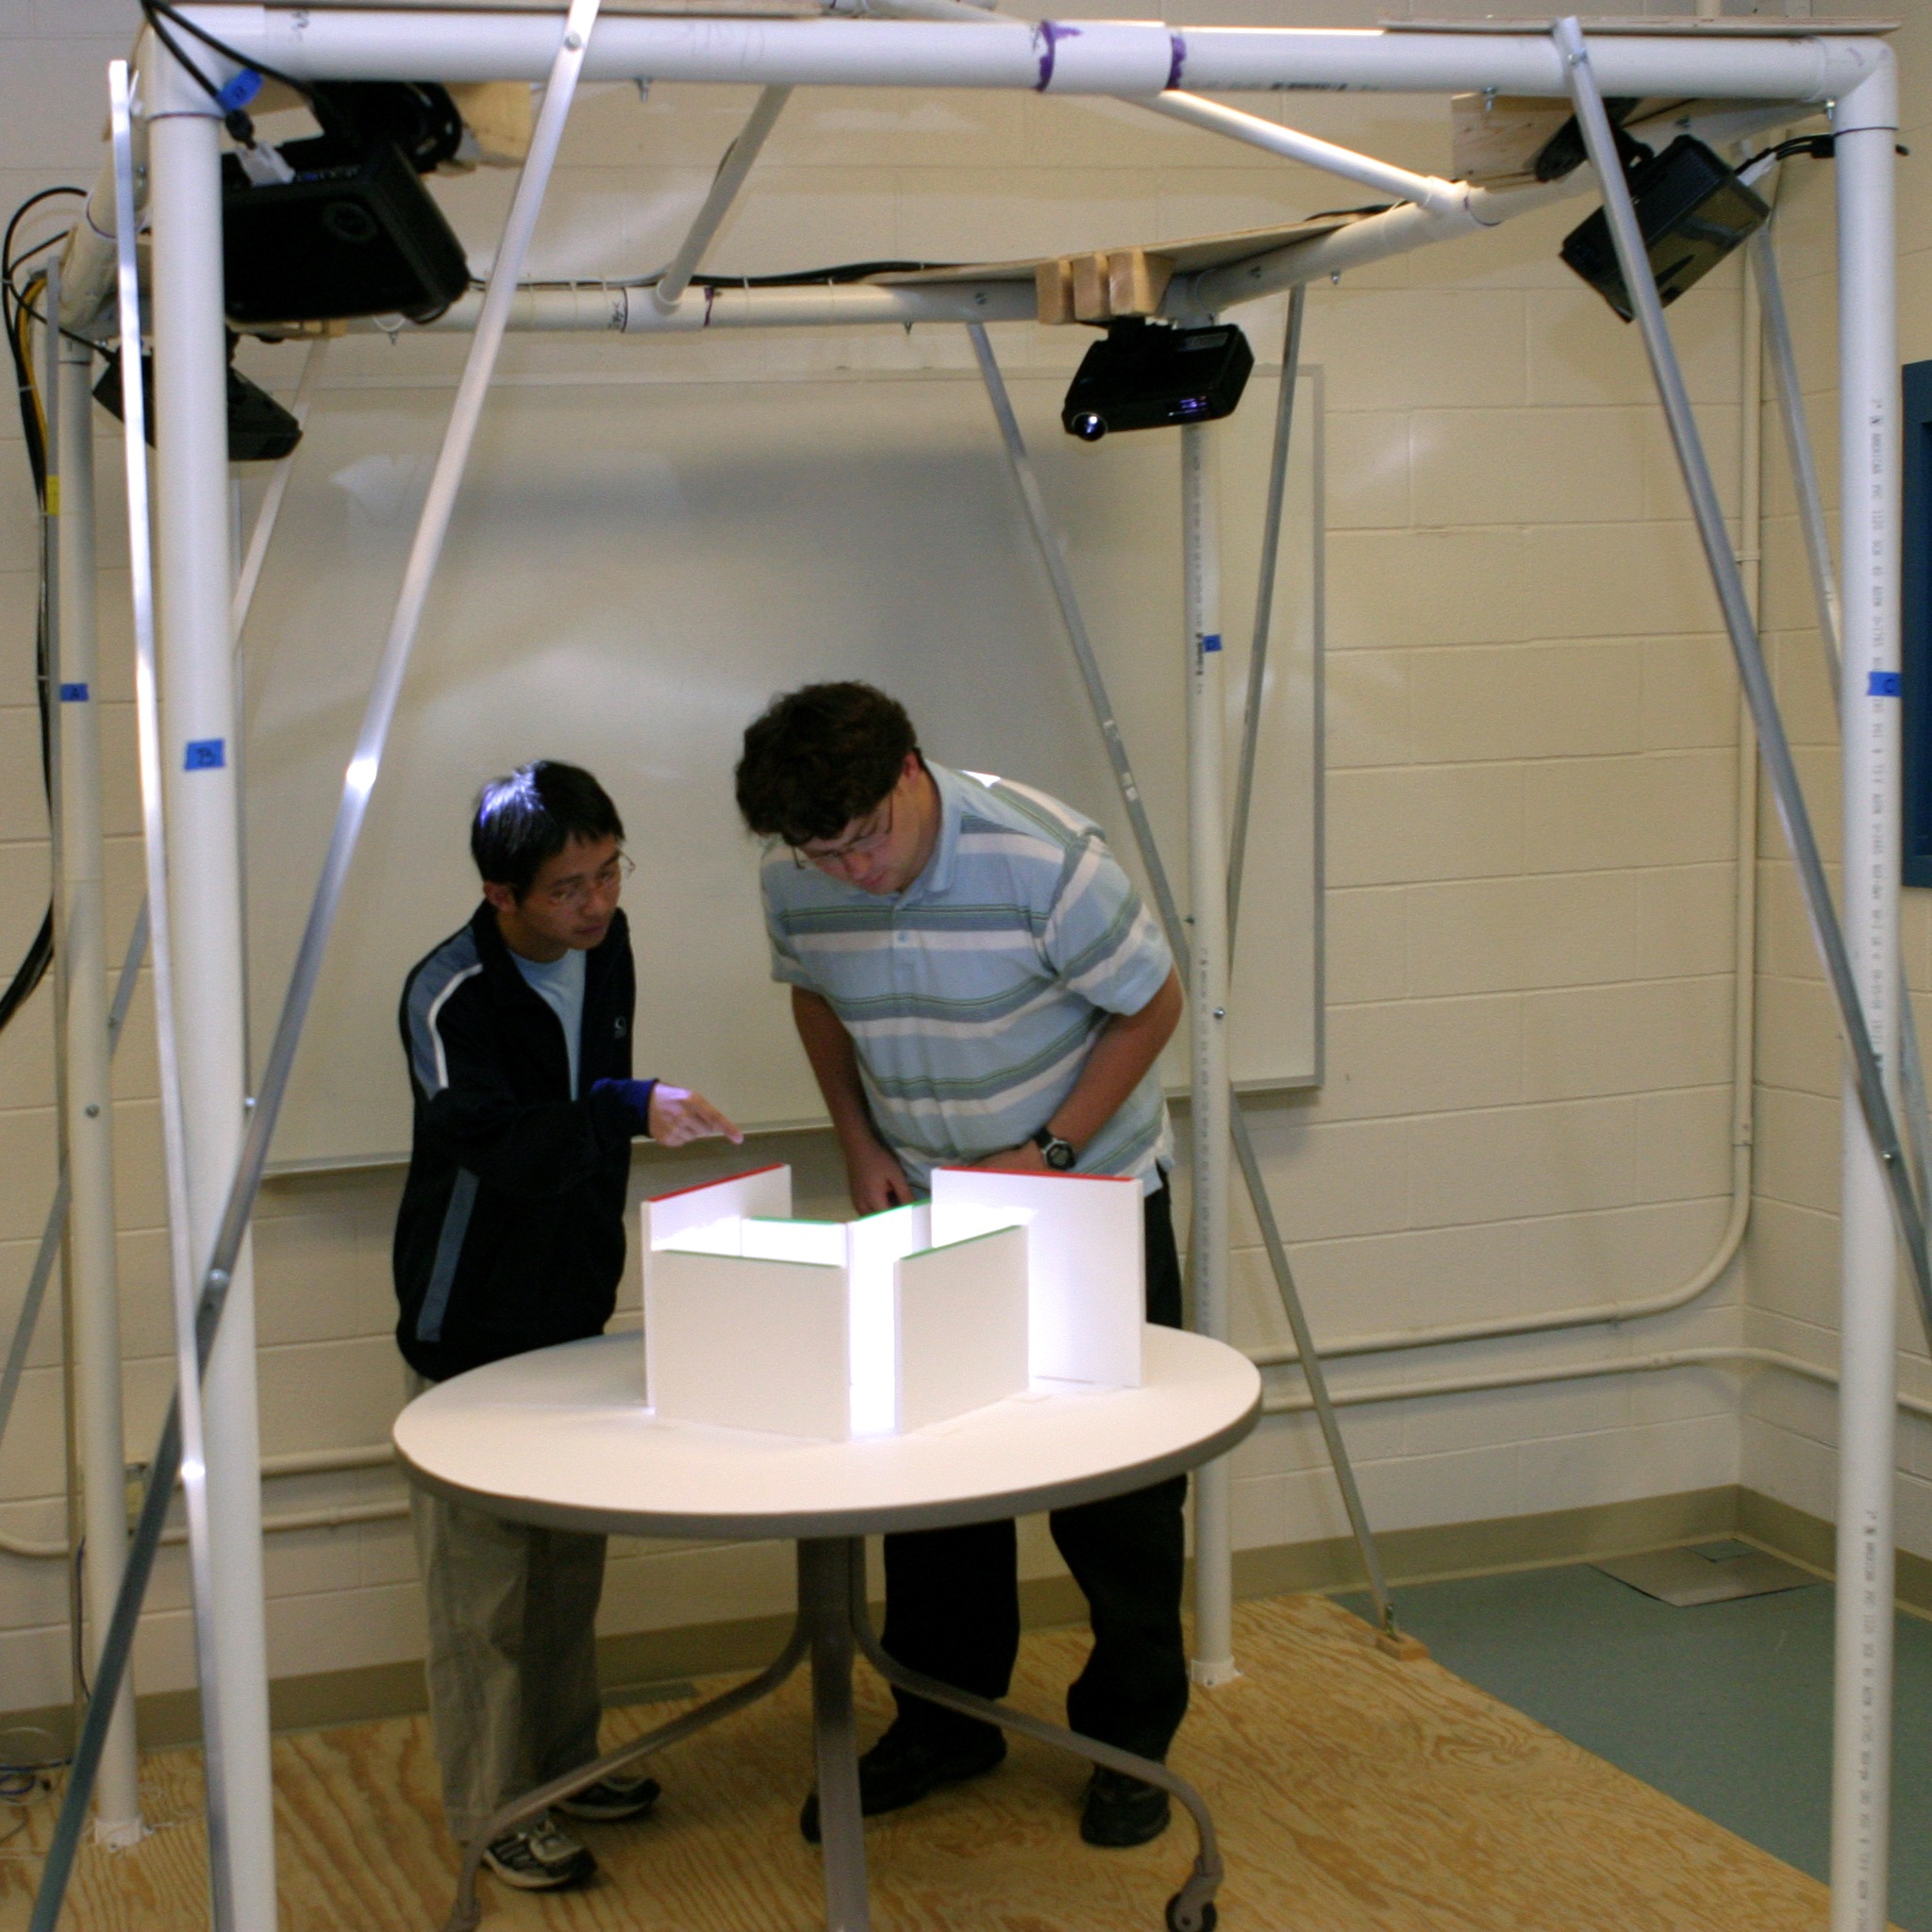
\includegraphics{aag2010_images/yu_stuetzle_contraption}}
\resizebox{!}{0.98in}{\includegraphics{aag2010_images/cshape_slr_model}}
\resizebox{!}{0.98in}{\includegraphics{aag2010_images/cshape_annotated}}
\resizebox{!}{0.98in}{\includegraphics{aag2010_images/remesher_cshape}}
\vspace{-0.2in}
\\
\begin{minipage}{0.98in}\textcolor[rgb]{1,1,1}{\hspace{-0.01in} {\bf a)}} \end{minipage}
\begin{minipage}{1.30in}\textcolor[rgb]{0,0,0}{\hspace{-0.01in} {\bf b)}} \end{minipage}
\begin{minipage}{0.98in}\textcolor[rgb]{1,1,1}{\hspace{-0.01in} {\bf c)}} \end{minipage}
\begin{minipage}{1.20in}\textcolor[rgb]{0,0,0}{\hspace{-0.01in} {\bf d)}} \end{minipage}
\caption{In our physical architectural design environment a) users
  gather around a table and construct b) a small-scale mockup of a
  design from a collection of wall elements and marker tokens.  A
  camera above the table c) captures the layout of elements on the
  table.  Our sketch interpretation algorithm processes these elements
  to construct a consistent and watertight triangular mesh of the
  implied architectural design (ceiling removed for visualization). }
\label{figure:virtual_heliodon}
\end{figure}

%%%%%%%%%%%%%%%%%%%%%%%%%%%%%%%%%%%%%%%%%%%%%%%%%%%%%%%%%%%%%%%%%%%%%%%%
%\subsection{Contributions}

%In this paper we present the following contributions:

%\begin{itemize}

%\item The collection of several hundred physical architectural
%  sketches using our design environment.  Each design is annotated by
%  the original designer to indicate the intended interpretation of the
%  design.

%\item Re-interpretation of these designs by other humans to provide a
%  measure of the ambiguity present in these sketches.  The set of
%  human interpretations is compared to the algorithm's output for
%  validation.

%\end{itemize}

%\subsection{Overview}

%We summarize several important areas of related work in
%Section~\ref{section:related_work}.  In
%Section~\ref{section:sketch_interpretation} we present our sketch
%interpretation algorithm, which was developed with extensive user testing
%and feedback from both architects and non-architects.  In
%Section~\ref{section:user_study} we present the results of two formal user
%studies that we conducted to gather a large set of example designs and
%validate our sketch interpretation approach.

\begin{comment}
%%%%%%%%%%%%%%%%%%%%%%%%%%%%%%%%%%%%%%%%%%%%%%%%%%%%%%%%%%%%%%%%%%%%%%%%
\section{Related Work}

\label{section:related_work}

Our project draws from research in a wide variety of areas including:
sketching interfaces, sketch recognition, human perception, and
computational models of gestalt and saliency.  In the sections below
we provide a brief overview of prior art in these fields and existing
software for architectural design.

\subsection{Modeling Interfaces for Architectural Design}

Many existing computer software packages tackle the challenge of
constructing 3D architectural geometry.  Initially these packages
focused almost exclusively on creating models with high geometric
precision, requiring a significant investment of time and only limited
support for editing a completed model.  Unfortunately, because
focusing on precision too early in the design process can stifle
creativity~\cite{LAWSON}, these tools are generally used only in the
later stages of design.  

The requirements for 3D models in architecture vary tremendously
depending on the intended use of the model.  Photorealistic renderings
require high polygon count geometry and accurate normals and
materials.  In contrast, many simulations (e.g., acoustic, passive
ventilation, heating/cooling, structural analysis) require a
consistent and watertight geometric model for accurate calculations
and often perform most efficiently with a simplified model constructed
especially for that analysis~\cite{ecotect}.  

More recently, software tools have become more amenable to the fast-paced,
quick sketching of the early stages of design~\cite{sketchup}, including
explorations of pen-based user interfaces for 3D
modeling~\cite{Zeleznik:1996:SAI,teddy,And02correlation-basedreconstruction}.
A limited construction interface (axis-aligned elements on a floor plan
grid) can help ensure the construction of architectural environments that
are appropriate for use in virtual reality walkthroughs~\cite{mackie}.  New
drawing user interfaces and systems have been demonstrated that allow
architects to leverage their pen and paper skills when interacting with the
new media interface of the computer.  Using projective geometry, freehand
architectural sketches can be re-projected or warped to simulate novel
viewpoints and an immersive experience~\cite{tolba}.  The Mental Canvas
system allows designers to arrange 2D sketches on arbitrary planes in 3D,
constructing an effective representation of complex architectural
spaces~\cite{mental_canvas}.




%-----------------
\subsection{\bf Sketch Recognition}

Sketch recognition systems are typically custom-developed for each
application (e.g., recognizing hand drawn UML
diagrams~\cite{UML_diagrams}) and leverage domain-specific knowledge
to improve accuracy.  General-purpose toolkits and languages for
sketch recognition of diagram components can ease the development of
these programs~\cite{ladder}.  

Well-designed sketching user interfaces minimize the number of
times the user is prompted for additional information or design
annotation, which interrupts workflow and concentration.  Strategies
for continuous and incremental recognition of drawings as they develop
have been demonstrated~\cite{Alvarado01resolvingambiguities}.  It is
important to maintain an estimate of the confidence in the
intermediate interpretations, which improves the accuracy of the final
interpretation.
%sketch interpretation in real time, but with
%limited interruptions of the user to ask if the interpretation is
%correct.  incremental interpretation, interpretation revision in the
%presence of new sketch data
An ongoing challenge in sketch recognition is the grouping of multiple
individual strokes that form a single logical unit.  The drawing
sequence for individual strokes and other meta-data available from
tablet displays~\cite{wacom} can be used as evidence when tackling
this problem~\cite{gross_1994}.  Another challenge in sketch
recognition comes from touch-up or continuation strokes the user might
make to complete a drawing~\cite{paulson_phdthesis}.  These strokes
are disconnected from or overlap other strokes but are intended to be
recognized as a single object.  Spatially close strokes (often defined
as the distance between two endpoints being less than 10\% of their
average length) can be merged; however this greedy approach, while
fast enough for interactive sketching, is not optimal.
%Overtraced strokes are still challenging to detect and
%recognize and accuracy drops with complex shapes.  A hierarchical
%analysis of subshapes has potential.

%Principles of sketch recognition require understanding of the

%* confidence level reflects sketch recognition accuracy

\subsection{\bf Sketch Recognition for Architectural Drawings}

The precision, consistency, and standardization of architectural CAD
drawings make this domain amenable to automatic processing algorithms,
and an impressive collection of automated sketch recognition programs
have been developed for architectural
drawings~\cite{Ah-soon97variationson,architectural_symbol_recognition,kulikov_mastersthesis,Lu_electronic_architectural_drawings}.
The motivation behind many of these tools is the digitization and
automated reconstruction of 3D building geometry from older
construction documents.  These methods have also been demonstrated for
hand-drawn architectural designs that closely follow the diagrammatic
conventions of CAD
drawings~\cite{aoki_hand_sketched_floor_plans,llados_hough}. For
example, the VR Sketchpad project automatically interprets a 2D
floorplan sketch including furniture layout to create a 3D VRML model
that can be used for walkthroughs~\cite{vrsketchpad}.  Freehand
sketching can be used to interact with digital
models~\cite{Gross00drawingon} and preliminary work was done to
classify interior and exterior walls in quick floorplan
sketches~\cite{archiassist}.

Koutamanis and Mitossi describe three levels of automated recognition
of architectural floor plans: recognition of geometric elements,
recognition of building elements, and recognition of spatial
articulation \cite{Koutamanis_computer_vision}.  They argue that the
third category is the most advanced: identifying solid mass versus
space within the design.  Our aim in this work is to specifically
address this challenge for freeform architectural sketches using a
tangible interface.
%Koutamanis discusses strategies to represent uncertainty in design
%within digital models~\cite{koutamanis_fuzzy}.  


%----------------------------
\subsection{Gestalt Theory and Sketch Interpretation}

Gestalt psychology, the laws of perceptual organization, and
Pragnanz~\cite{koffka,kanizsa} describe how humans perceive and
interpret incomplete diagrams or other modes of partial stimuli.  The
fundamental phenomena of closure, proximity, symmetry, and continuity
can be explained by low level human vision processing.  Gestalt theory
describes why our interpretation of an incomplete or ambiguous diagram
tends toward simpler forms, avoiding complexity.  The rich vocabulary
of pen and paper sketching in architectural design draws on the
gestalt principles of collinearity, parallelism, continuation, and
completion~\cite{koutamanis_sketch_recognition}.  Our algorithm for
automated interpretation of architectural sketches follows and
implements these principles.  Our user studies on human interpretation
of architectural sketches provides validation to our proposed use of
these concepts in recognition and analysis of architectural designs.

Research in computer vision has developed algorithms for image
processing using computational models of gestalt.  Attributes which
define the form, i.e., thickness of a line, convexity, and
parallelism, can be referred to as {\em gestalts}~\cite{desol02}.
Computational gestalt research focuses on determining thresholds that
indicate a pattern is significant.  In other words, this work involves
detecting and studying patterns and analyzing how likely those
patterns would be to occur in the image randomly~\cite{desol02}.
%While
%we are not explicitly using computational gestalt in our algorithm we
%do use something very similar to it in order to interpret the designs.
%We have to do a similar analysis to computational gestalt to decide if
%walls are meant to be collinear.

Similarly, saliency is a measure of how much an area stands out in
comparison to the areas around it. 
%
A {\em saliency map}~\cite{koch85} combines different stimuli
(movement, color, etc.) and the relative conspicuity to quantify changes 
in these characteristics.
%Detecting salient areas of an
%image is an important in Computer Vision.  
Itti, Koch and Niebur designed a computational visual attention model
based on the primate visual system to estimate the saliency map and
identify which areas of the scene are most likely to contain useful
information and should be analyzed in more detail~\cite{itti98}.
%
%~\cite{siag} 
%Saliency to aid in their robot localization system.
%Along with finding the "gist" of the scene, salient regions are used
%in a Monte-Carlo method to deduce it's location.
%Research continues to be
%done using Saliency such as Decarlo who created a program that
%transforms a photo into a line drawing by tracking a user's eye
%movements and keeping the most detail where the user focuses
%~\cite{decarlo02}. 
%Research has also been continuing on finding faster
%ways to obtain saliency maps such as using GPU's ~\cite{long06}.


%%%%%%%%%%%%%%%%%%%%%%%%%%%%%%%%%%%%%%%%%%%%%%%%%%%%%%%%%%%%%%%%%%%%%%%%
\section{Sketch Interpretation Algorithm}

\label{section:sketch_interpretation}

In our physical sketching environment, the user selects from the provided
collection of physical props and quickly assembles the chosen pieces on the
table.  Thus, the arrangement of elements truly forms a rough, approximate
sketch.  The selected wall pieces are likely too long or too short,
yielding overlaps or gaps with adjacent walls.  Similarly, the limited
palette of curved components may not have the desired curvature and thus
tangential connections are imprecise.  Furthermore, the approximate
assembly manner means that components intended to be parallel or meet at
crisp $90\,^{\circ}$ angles will include some unavoidable imprecision.  The
challenge is to sift through the available information to deduce and
construct the clean and complete design as it was conceived in the
architect's mind.

In the following sections we present the key steps of our sketch
interpretation algorithm: image pre-processing, detecting parallel,
perpendicular, and collinear elements, linking elements into chains,
constructing an arrangement of polygonal cells, estimating spatial
enclosure, assigning interior/exterior zones, managing details, and
post-processing the floorplan geometry to make a 3D model.

%------------------------------------------------
\subsection{Image Pre-Processing}

A camera mounted above the table captures the details of the physical
sketch.  A controlled lighting environment and carefully chosen color-coded
labels on the physical elements allow this geometry to be robustly
detected using standard image processing techniques, which are described in
detail in our earlier publications~\cite{virtual_heliodon,tvcg2009}.

The input to our sketch interpretation algorithm is the 2D projection
of each detected wall module onto the table surface, labeled with the
element height.  The flat walls are rectangles and include any
associated windows as inscribed rectangles.  The circular arc curved
walls are specified by a center, the inner and outer radii, and the
start and end angles of the arc.  An example of this input is shown in
Figure~\ref{figure:colinearity}a.


%------------------------------------------------
\subsection{Intended Parallel, Perpendicular, and Collinear Elements}
\end{comment}
\begin{figure}[t]
\resizebox{0.74in}{0.74in}{\includegraphics{aag2010_images/colinearity_tolerance/20091028_00636_2D_walls}}
\resizebox{0.74in}{0.74in}{\includegraphics{aag2010_images/colinearity_tolerance/20091028_annotated_00636}}
\resizebox{0.74in}{0.74in}{\includegraphics{aag2010_images/colinearity_tolerance/20091028_00636_interp_026}}
\resizebox{0.74in}{0.74in}{\includegraphics{aag2010_images/colinearity_tolerance/20091028_00636_interp_033}}
\resizebox{0.74in}{0.74in}{\includegraphics{aag2010_images/colinearity_tolerance/20091028_00636_interp_036}}
\resizebox{0.74in}{0.74in}{\includegraphics{aag2010_images/colinearity_tolerance/20091028_00636_interp_075}}
%\resizebox{0.63in}{0.63in}{\includegraphics{aag2010_images/colinearity_tolerance/20091028_00636_floorplan}}
\vspace{-0.36in}
\\
\begin{minipage}{0.74in}\textcolor[rgb]{0,0,0}{\hspace{-0.01in} { a)}} \end{minipage}
\begin{minipage}{0.74in}\textcolor[rgb]{0,0,0}{\hspace{-0.01in} { b)}} \end{minipage}
\begin{minipage}{0.74in}\textcolor[rgb]{0,0,0}{\hspace{-0.01in} { c)}} \end{minipage}
\begin{minipage}{0.74in}\textcolor[rgb]{0,0,0}{\hspace{-0.01in} { d)}} \end{minipage}
\begin{minipage}{0.74in}\textcolor[rgb]{0,0,0}{\hspace{-0.01in} { e)}} \end{minipage}
\begin{minipage}{0.74in}\textcolor[rgb]{0,0,0}{\hspace{-0.01in} { f)}} \end{minipage}
\caption{Intended collinearity can be ambiguous: a) detected primitives, b)
  annotation by the original designer, and c-f) annotation by other users.}
\label{figure:colinearity}
\end{figure}
 
\begin{comment}
For practical construction and space efficiency reasons, most
real-world architecture involves parallel walls and sharp
$90\,^{\circ}$ corners.  Even within high-profile showpiece
architecture, spaces are typically arranged into regular patterns and
placed on a grid, sometimes with secondary grids that are offset
and/or rotated.  Many (but not all) designs created by participants
using our tangible sketching interface follow these conventions and we
can automatically detect the implied grid(s).

First, we cluster the flat walls into groups that are nearly parallel
and {\em snap} all walls in each group to their weighted average
direction.  Similarly, we compare the wall groups to each other and
those that are approximately perpendicular are snapped to be
orthogonal.  We found that an angle tolerance of $5\,^{\circ}$ was an
appropriate threshold across all of our collected design data.  This
tolerance was effective at cleaning up placement imprecision inherent
in the physical sketching environment, yet was not large enough to
introduce artifacts in the more freeform designs that eschewed
parallelism and right angles.

In addition to the angle tolerance, it is necessary to identify flat
walls that are approximately collinear.  However, selecting a global
setting for this offset tolerance distance is somewhat more difficult.
We also saw variable tolerances for collinearity in human perception
when different users were asked to interpret the same design
(Figure~\ref{figure:colinearity}).  Some users perceived a slight line
break as an intended straight line, while others interpreted the break
as an architectural feature and possibly an entrance.  We found that
using a 1'' offset distance tolerance in our physical sketching
environment (equal to 1' in full-scale) was a good compromise for our
automatic collinearity detection and adjustment, but the user may need
control of this threshold for some designs.


We have not yet finished implementation of similar clustering and
adjustment methods for circular arcs.  The implementation is
straightforward and will require determination of appropriate
tolerances and smoothing procedures for several cases: multiple arcs
placed to sketch a circle or ellipse (e.g.,
Figure~\ref{figure:colinearity}), two arcs that form an inflection
point, and adjustment of the tangent and/or curvature when a circular
arc leads into a flat, straight wall.

%------------------------------------------------
\subsection{Linking Walls to Form Continuous Chains}

Following the gestalt principle of continuity we not only snap nearly
collinear elements to a common line, but we also form explicit
connections between elements with similar tangents (straight to
straight, straight to curved, or curved to curved).  Two or more
elements can be connected into a {\em chain} that is traced through
the working plane, separating space into two regions.  Our angular and
offset distance tolerances for establishing a connection between two
elements is less strict than the parallel and collinear thresholds
described in the previous section, allowing the establishment of
longer freeform chains.  Examples of these chains are shown in
Figure~\ref{figure:cells}c.

Our algorithm for establishing the chains is as follows.  For each
endpoint of each wall element we search all other walls for the best
matching connection tangent.  If a pairwise connection is mutual
(element A selects element B as the best match for tangent direction
and offset distance and element B also selects element A as the best
match), then the connection is established.  If no connection is made
for a wall endpoint, then that end of the wall chain is simply
extended to infinity following the tangent of the wall at that
endpoint.  When a wall chain connects curved arcs, the chain may form
a U turn (Figure~\ref{figure:cells} second row), a closed loop
(Figure~\ref{figure:cells} third row), or other interesting shapes.
\end{comment}
\begin{figure}[t]
\resizebox{0.74in}{0.74in}{\includegraphics{aag2010_images/arrangement_examples/091_02766_2D_walls}}
\resizebox{0.74in}{0.74in}{\includegraphics{aag2010_images/arrangement_examples/091_annotated_02766}}
\resizebox{0.74in}{0.74in}{\includegraphics{aag2010_images/arrangement_examples/091_02766_wall_chains}}
\resizebox{0.74in}{0.74in}{\includegraphics{aag2010_images/arrangement_examples/091_02766_fingerprint}}
\resizebox{0.74in}{0.74in}{\includegraphics{aag2010_images/arrangement_examples/091_02766_enclosed_points}}
\resizebox{0.74in}{0.74in}{\includegraphics{aag2010_images/arrangement_examples/091_02766_floorplan}}\\
%
\resizebox{0.74in}{0.74in}{\includegraphics{aag2010_images/arrangement_examples/20091021_01108_2D_walls}}
\resizebox{0.74in}{0.74in}{\includegraphics{aag2010_images/arrangement_examples/20091021_annotated_01108}}
\resizebox{0.74in}{0.74in}{\includegraphics{aag2010_images/arrangement_examples/20091021_01108_wall_chains}}
\resizebox{0.74in}{0.74in}{\includegraphics{aag2010_images/arrangement_examples/20091021_01108_fingerprint}}
\resizebox{0.74in}{0.74in}{\includegraphics{aag2010_images/arrangement_examples/20091021_01108_enclosed_points}}
\resizebox{0.74in}{0.74in}{\includegraphics{aag2010_images/arrangement_examples/20091021_01108_floorplan}}\\
%
\resizebox{0.74in}{0.74in}{\includegraphics{aag2010_images/arrangement_examples/091_13151_2D_walls}}
\resizebox{0.74in}{0.74in}{\includegraphics{aag2010_images/arrangement_examples/091_annotated_13151}}
\resizebox{0.74in}{0.74in}{\includegraphics{aag2010_images/arrangement_examples/091_13151_wall_chains}}
\resizebox{0.74in}{0.74in}{\includegraphics{aag2010_images/arrangement_examples/091_13151_fingerprint}}
\resizebox{0.74in}{0.74in}{\includegraphics{aag2010_images/arrangement_examples/091_13151_enclosed_points}}
\resizebox{0.74in}{0.74in}{\includegraphics{aag2010_images/arrangement_examples/091_13151_floorplan}}\\
%
\resizebox{0.74in}{0.74in}{\includegraphics{aag2010_images/arrangement_examples/20091021a_00131_2D_walls}}
\resizebox{0.74in}{0.74in}{\includegraphics{aag2010_images/arrangement_examples/20091021a_annotated_00131}}
\resizebox{0.74in}{0.74in}{\includegraphics{aag2010_images/arrangement_examples/20091021a_00131_wall_chains}}
\resizebox{0.74in}{0.74in}{\includegraphics{aag2010_images/arrangement_examples/20091021a_00131_fingerprint}}
\resizebox{0.74in}{0.74in}{\includegraphics{aag2010_images/arrangement_examples/20091021a_00131_enclosed_points}}
\resizebox{0.74in}{0.74in}{\includegraphics{aag2010_images/arrangement_examples/20091021a_00131_floorplan}}
\\
\resizebox{0.74in}{0.74in}{\includegraphics{aag2010_images/graphcut_example/088_08661_2D_walls}}
\resizebox{0.74in}{0.74in}{\includegraphics{aag2010_images/graphcut_example/088_annotated_08661}}
\resizebox{0.74in}{0.74in}{\includegraphics{aag2010_images/graphcut_example/088_08661_wall_chains}}
\resizebox{0.74in}{0.74in}{\includegraphics{aag2010_images/graphcut_example/088_08661_fingerprint}}
\resizebox{0.74in}{0.74in}{\includegraphics{aag2010_images/graphcut_example/088_08661_enclosed_points}}
\resizebox{0.74in}{0.74in}{\includegraphics{aag2010_images/graphcut_example/088_08661_floorplan}}
\vspace{-0.35in}
\\
\begin{minipage}{0.74in}\textcolor[rgb]{0,0,0}{\hspace{-0.01in} { a)}} \end{minipage}
\begin{minipage}{0.74in}\textcolor[rgb]{0,0,0}{\hspace{-0.01in} { b)}} \end{minipage}
\begin{minipage}{0.74in}\textcolor[rgb]{0,0,0}{\hspace{-0.01in} { c)}} \end{minipage}
\begin{minipage}{0.74in}\textcolor[rgb]{0,0,0}{\hspace{-0.01in} { d)}} \end{minipage}
\begin{minipage}{0.74in}\textcolor[rgb]{0,0,0}{\hspace{-0.01in} { e)}} \end{minipage}
\begin{minipage}{0.74in}\textcolor[rgb]{0,0,0}{\hspace{-0.01in} { f)}} \end{minipage}
\caption{Dividing space into cells by extending tangents and connecting
  elements:  a) detected primitives, b) annotation by original designer,
  c) wall chains, d) zones defined by the wall chains, e) enclosure, and f)
  our automatic interpretation. }
\label{figure:cells}
\end{figure}
\begin{comment}
Defined spaces in architecture can be created by real and/or implied
boundaries.  Each wall chain divides the working plane into two
spaces, one on either ``side'' of the chain.  The set of all wall
chains in a model will divide space into many subspaces that can be
labeled by their sidedness, which is visualized in
Figure~\ref{figure:cells}d.  If a wall chain loops around and crosses
itself (Figure~\ref{figure:cells} fourth row, blue and yellow chains),
the loop portion of the chain is disconnected to define a new chain to
allow the unique labeling of all subspaces.  Note that if two wall
chains cross two or more times (which is possible if one or both
chains are non-linear), the resulting subspace organization may have
two disconnected spaces that have the same sidedness
(Figure~\ref{figure:cells} fifth row, blue and red cells).  We perform
a connected component analysis to identify this situation and define
separate subspaces.

%------------------------------------------------
\subsection{Arrangement of Cells and Enclosure}

The wall chains described in the previous section are used to cut the
working plane into a watertight planar convex polygonal mesh or
arrangement of cells, which is represented using a half-edge data
structure.  Each wall chain explicitly represents the wall thickness,
thus working plane polygons are constructed for both open space
(interiors and exteriors) as well as the are comprising the
construction thickness of real and implied walls.

For each cell in the arrangement, we calculate the {\em enclosure},
the probability that the cell is part of the building interior.  We
define the enclosure at a point as the lack of visibility to areas
outside of the design from that point.  We estimate this value by
tracing rays from the point to infinity in a dense sampling of
directions and record the fraction of all rays that intersect a wall
of the design.  We visualize enclosure over a dense point grid in
Figure~\ref{figure:cells}d.  Points with high enclosure (nearly all
rays intersect a wall in the design) are drawn light grey or white,
and points with low enclosure are dark grey.  We define the average
enclosure of the cell in the arrangement by averaging the enclosure at
many points within the cell.  Similarly, we can compute the average
and standard deviation of the point-based enclosure values for a
subspace.

For relatively simple designs, a carefully-selected global threshold
placed on the point/cell/subspace enclosure value can correctly
classify each subspace as interior or exterior.  However, as the gaps
between the walls increase or decrease the threshold value must be
adjusted accordingly (compare the first and third rows of
Figure~\ref{figure:cells}d).  Furthermore, if the model contains
concavities in the outer wall, nearby areas may be incorrectly marked
as interior spaces.  Beyond the challenge of selecting a threshold,
for more complex models a simplistic setting of a global threshold
will not successfully separate the building interior from exterior
(Figure~\ref{figure:nonconvex}).

One cause for incorrect interior/exterior division is high variance in
enclosure within a single subspace.  For example, consider the final row of
Figure~\ref{figure:cells}.  The sharp bends of the blue wall chain loop
through the design and interact with the other two wall chains to produce
one large subspace, colored cyan and green.  The enclosure values within
this subspace have high variance, indicating that it should not be treated
as a single space when identifying interior space.  For each subspace with
high enclosure variance, we solve a Minimum Cut graph problem to determine
an optimal segmentation of this subspace.  We build a dual graph from the
polygonal cells in this subspace.  Each polygonal cell in the arrangement
is a node in the graph.  If two cells share an edge in the arrangement, we
create an edge between the corresponding nodes in the graph.  The weight of
the edge is defined to be the length of the shared edge in the arrangement.
The source is defined to be the node whose corresponding cell has the
highest enclosure, and the sink is likewise defined to be the cell with the
lowest enclosure value.  Using a basic textbook implementation of the
Maximum Flow/Minimum Cut algorithm, we find a minimum length cut which
divides the zone into two subspaces that will have lower variance and
produce a more satisfactory interior/exterior segmentation of the design.
\end{comment}
\begin{figure}[t]

\resizebox{0.74in}{0.74in}{\includegraphics{aag2010_images/courtyard/20091014_annotated_03526}}
\resizebox{0.74in}{0.74in}{\includegraphics{aag2010_images/courtyard/20091014_03526_enclosed_points}}
\resizebox{0.74in}{0.74in}{\includegraphics{aag2010_images/courtyard/20091014_03526_floorplan}}
%
\resizebox{0.74in}{0.74in}{\includegraphics{aag2010_images/courtyard/040_annotated_07372}}
\resizebox{0.74in}{0.74in}{\includegraphics{aag2010_images/courtyard/040_07372_enclosed_points}}
\resizebox{0.74in}{0.74in}{\includegraphics{aag2010_images/courtyard/040_07372_floorplan}}
\\
\resizebox{0.74in}{0.74in}{\includegraphics{aag2010_images/courtyard/066_annotated_03260}}
\resizebox{0.74in}{0.74in}{\includegraphics{aag2010_images/courtyard/066_03260_enclosed_points}}
\resizebox{0.74in}{0.74in}{\includegraphics{aag2010_images/courtyard/066_03260_floorplan}}
%
\resizebox{0.74in}{0.74in}{\includegraphics{aag2010_images/courtyard/20091014_annotated_02020}}
\resizebox{0.74in}{0.74in}{\includegraphics{aag2010_images/courtyard/20091014_02020_enclosed_points}}
\resizebox{0.74in}{0.74in}{\includegraphics{aag2010_images/courtyard/20091014_02020_floorplan}}
\caption{Designs with non convex boundaries may not be accurately
  extracted with a simple threshold on the average point or cell
  enclosure.  By minimizing the lengths of unused wall and extra {\em
    inferred wall} necessary to enclose the interior zones we 
  correctly interpret these complex designs.}
\label{figure:nonconvex}
\end{figure}

\begin{comment}
%------------------------------------------------
\subsection{Assigning Interior and Exterior Zones}


After the wall chains have divided the working plane into a set of
zones, we need to label each zone as either an interior or exterior
space.  The average enclosure value for the zone can be used to make
an initial determination, but that strategy frequently yields
incorrect assignments for complex designs with non-convex boundaries
(e.g., Figure~\ref{figure:multiple_rooms}).  Furthermore, our method
for constructing wall chains that extend each element to infinity will
yield a division of space into zones far from the element's actual
position, which may not be intended.  When two neighboring zones are
assigned opposite labels, the wall or wall chain between the zone is
thus interpreted as an implied wall or boundary.  If the original wall
element is short and/or a significant distance from the implied
boundary, the resulting automatically-constructed floor plan may be
non intuitive and not match a human interpretation.  Therefore, we
must be careful to use an extended wall chain as evidence for a
boundary only in close proximity to the original wall.  Every
hypothesized or inferred wall separating interior and exterior space
should be checked against the evidence.
\end{comment}
\begin{figure}[t]
\resizebox{0.74in}{0.74in}{\includegraphics{aag2010_images/multiple_rooms_examples/20091028_00908_2D_walls}}
\resizebox{0.74in}{0.74in}{\includegraphics{aag2010_images/multiple_rooms_examples/20091028_annotated_00908}}
\resizebox{0.74in}{0.74in}{\includegraphics{aag2010_images/multiple_rooms_examples/20091028_00908_floorplan}}
%
\resizebox{0.74in}{0.74in}{\includegraphics{aag2010_images/multiple_rooms_examples/013_03253_2D_walls}}
\resizebox{0.74in}{0.74in}{\includegraphics{aag2010_images/multiple_rooms_examples/013_annotated_03253}}
\resizebox{0.74in}{0.74in}{\includegraphics{aag2010_images/multiple_rooms_examples/013_03253_floorplan}}
%
\resizebox{0.74in}{0.74in}{\includegraphics{aag2010_images/multiple_rooms_examples/013_01221_2D_walls}}
\resizebox{0.74in}{0.74in}{\includegraphics{aag2010_images/multiple_rooms_examples/013_annotated_01221}}
\resizebox{0.74in}{0.74in}{\includegraphics{aag2010_images/multiple_rooms_examples/013_01221_floorplan}}
%
\resizebox{0.74in}{0.74in}{\includegraphics{aag2010_images/multiple_rooms_examples/013_05156_2D_walls}}
\resizebox{0.74in}{0.74in}{\includegraphics{aag2010_images/multiple_rooms_examples/013_annotated_05156}}
\resizebox{0.74in}{0.74in}{\includegraphics{aag2010_images/multiple_rooms_examples/013_05156_floorplan}}
%
\vspace{-0.25in}
\caption{
Challenging examples of designs with multiple rooms.  The
  examples in the bottom row are somewhat ambiguous and have multiple
  reasonable interpretations for the passageways between rooms. 
\vspace{-0.1in}
 }
\label{figure:multiple_rooms}
\end{figure}
\begin{comment}

In solving this problem, we follow the Gestalt principles of closure
and simplicity.  We search for a closed form that is simple, uses most
or all of the detected wall elements, and requires little length of
additional inferred exterior wall to fill gaps between the original
wall primitives of the sketch.  We solve this optimization problem in
a brute force manner by considering as interior space all subsets of
the zones with enclosure values above a reasonable threshold and
select the zone assignment that minimizes the sum of all unused walls
and all inferred walls.  An unused wall is defined as a detected
element that has exterior zone on both sides.  Note that wall elements
may be partially used and the unused wall penalty is accordingly
prorated.  Similarly, an inferred wall is a portion of wall chain that
is not represented in the sketch by a physical wall, but has exterior
zone on one side and interior zone on the other.  In the floor plan
results diagrams used throughout this paper, real walls are drawn in
black, interior zones are drawn in medium grey, exterior zones are
white and inferred walls are drawn in dark red for visualization
purposes.


Some of the collected designs contain an interior space that might
have been conceived as an open courtyard rather than a room with no
exterior walls (Figure~\ref{figure:courtyards}).  This distinction can
be important for architectural simulations such as daylighting design
or passive ventilation --- whether the finished design includes a roof
over this fully interior room will impact the simulated performance
results.  To resolve this ambiguity, we are considering user interface
options for allowing the designer to indicate which of these two
perfectly reasonable scenarios he/she intended.  Importantly, we want
maintain our minimalist interface and follow the most appropriate
default interpretation.

%------------------------------------------------
\subsection {Detecting Inferred Interior Walls and Trimming Unused Walls}

\begin{figure}[t]
\resizebox{0.74in}{0.74in}{\includegraphics{aag2010_images/courtyard/20091028_00772_interp_036}}
\resizebox{0.74in}{0.74in}{\includegraphics{aag2010_images/courtyard/20091028_00772_floorplan}}
%
\resizebox{0.74in}{0.74in}{\includegraphics{aag2010_images/courtyard/060_12354_interp_018}}
\resizebox{0.74in}{0.74in}{\includegraphics{aag2010_images/courtyard/060_12354_floorplan}}
%
\resizebox{0.74in}{0.74in}{\includegraphics{aag2010_images/courtyard/066_annotated_05996}}
\resizebox{0.74in}{0.74in}{\includegraphics{aag2010_images/courtyard/066_05996_floorplan}}
\caption{If the design contains a interior room with no exterior
  walls, this space may be intended as a courtyard space, uncovered by
  a roof. The system will require extra information from the designer
  if the default interpretation does not match his/her intentions. }
\label{figure:courtyards}
\end{figure}


Once the core interior/exterior spaces of the design have been
determined and the true exterior and inferred exterior walls have been
identified, the system performs several small cleanup steps to improve
the quality of the final model and ensure that the extracted 3D
geometry is manifold.
%
When two wall chains that each define a portion of the boundary
between interior and exterior cross, the quadrilateral zone defined by
the thickness of each chain at the crossing should also be labeled as
a wall to create proper interior and exterior corners.

Some designs incorporate interior partition walls that are meant to
separate the interior into smaller rooms.  Due to the physical
sketching environment, generally these walls are a bit short and leave
small gaps where they should meet other interior or exterior walls.
However, not all gaps should be closed.  Standard doorways in
architecture are generally a minimum of 2'6'' wide, so if the gap is
less than 2'' wide, we assume this was intended to be a solid wall and
we close the gap by labeling the corresponding wall chain polygons as
inferred walls.  We found that this tolerance provided a reasonable
match to the designer's annotation of his/her intentions for the full
range of example designs.
%
Similarly, when the physical wall modules are slightly too long and
protrude from the middle of an inferred boundary or corner, we should
clip back this geometry to create a more polished design.  We propose
a tolerance of 1'' (corresponding to 1' in full scale) for this
trimming.  We note that it is important to not completely remove from
the design all walls that are ``unused'' (not positioned on the
exterior/interior boundary of the model or used as interior
partitions).  In many cases these extra exterior walls serve specific
architectural functions including privacy screens, shading, acoustic
dampening, and wind control.

Finally, we propose an initial strategy for labeling the primary
entrance to a design, and augmenting the floorplan and 3D model with
this information.  Note that not all designs have a clear entrance,
but many of our user study participants left specific openings within
the outer boundary of their shape.  Simply detecting the longest
section of inferred exterior boundary (and greater than a minimum
tolerance of approximately 4'') as the primary entrance will correctly
label this feature in most of the designs.  One notable example that
breaks this rule is shown in the bottom row of
Figure~\ref{figure:domain_specific}.  Annotations made by other user
study participants match the intention of the original designer: the
obvious entrance is through an elaborate portico, rather than through
one of the large gaping holes in the ``back'' of the design.  This
sketch interpretation task will benefit from domain-specific knowledge
of common architectural forms.
\end{comment}
\begin{figure}[t]
\resizebox{0.74in}{0.74in}{\includegraphics{aag2010_images/domain_specific_examples/20091028a_annotated_00762}}
\resizebox{0.74in}{0.74in}{\includegraphics{aag2010_images/domain_specific_examples/20091028a_00762_interp_026}}
\resizebox{0.74in}{0.74in}{\includegraphics{aag2010_images/domain_specific_examples/20091028a_00762_interp_029}}
\resizebox{0.74in}{0.74in}{\includegraphics{aag2010_images/domain_specific_examples/20091028a_00762_interp_036}}
\resizebox{0.74in}{0.74in}{\includegraphics{aag2010_images/domain_specific_examples/20091028a_00762_interp_080}}
\resizebox{0.74in}{0.74in}{\includegraphics{aag2010_images/domain_specific_examples/20091028a_00762_floorplan}}
\\
\resizebox{0.74in}{0.74in}{\includegraphics{aag2010_images/domain_specific_examples/092-2_annotated_05027}}
%\resizebox{0.74in}{0.74in}{\includegraphics{aag2010_images/domain_specific_examples/092-2_05027_interp_017}}
\resizebox{0.74in}{0.74in}{\includegraphics{aag2010_images/domain_specific_examples/092-2_05027_interp_018}}
\resizebox{0.74in}{0.74in}{\includegraphics{aag2010_images/domain_specific_examples/092-2_05027_interp_026}}
\resizebox{0.74in}{0.74in}{\includegraphics{aag2010_images/domain_specific_examples/092-2_05027_interp_032}}
%\resizebox{0.74in}{0.74in}{\includegraphics{aag2010_images/domain_specific_examples/092-2_05027_interp_049}}
\resizebox{0.74in}{0.74in}{\includegraphics{aag2010_images/domain_specific_examples/092-2_05027_interp_067}}
\resizebox{0.74in}{0.74in}{\includegraphics{aag2010_images/domain_specific_examples/092-2_05027_floorplan}}
\vspace{-0.35in}
\\
\begin{minipage}{0.74in}\textcolor[rgb]{0,0,0}{\hspace{-0.01in} { a)}} \end{minipage}
\begin{minipage}{0.74in}\textcolor[rgb]{0,0,0}{\hspace{-0.01in} { b)}} \end{minipage}
\begin{minipage}{0.74in}\textcolor[rgb]{0,0,0}{\hspace{-0.01in} { c)}} \end{minipage}
\begin{minipage}{0.74in}\textcolor[rgb]{0,0,0}{\hspace{-0.01in} { d)}} \end{minipage}
\begin{minipage}{0.74in}\textcolor[rgb]{0,0,0}{\hspace{-0.01in} { e)}} \end{minipage}
\begin{minipage}{0.74in}\textcolor[rgb]{0,0,0}{\hspace{-0.01in} { f)}} \end{minipage}
\caption{Domain-specific knowledge may be necessary to correctly
  interpret sketches that hint at common architectural forms, such as
  the cruciform used in church floor plans (top row) or to recognize
  an entrance portico (bottom row).  Despite the potential for
  ambiguity, b-e) most users' interpretations matched a) the original
  designer's intention.  Our automatic sketch interpretation results
  are shown in f). }
\label{figure:domain_specific}
\end{figure}
\begin{comment}
%------------------------------------------------
\subsection{Post-Processing: Constructing a Watertight Triangle Mesh}

At the end of our sketch interpretation algorithm, we have a precise,
manifold, polygonal representation of the working plane.  Each
polygonal cell has well defined neighboring cells (no 'T' junctions)
and has been assigned one of several labels: {\em solid wall}, {\em
  window within a wall}, {\em interior space}, or {\em exterior
  space}.  This representation can be extruded and exported as a
consistent mesh following the necessary CAD conventions for
architectural rendering or performance simulation software.  For
example, we can construct a watertight mesh appropriate for a
radiosity simulation of interior illumination as follows.  Each
interior cell is exported as two polygons, one floor plane polygon
with normal pointing 'up' and one ceiling polygon with normal pointing
'down'.  For every edge between an interior cell and a wall or
exterior cell, we create a wall polygon stretching from the floor to
the ceiling with normal pointing toward the interior cell.  When an
interior cell touches a window cell, the exported wall polygon is
split vertically and assigned different materials as appropriate.


%%%%%%%%%%%%%%%%%%%%%%%%%%%%%%%%%%%%%%%%%%%%%%%%%%%%%%%%%%%%%%%%%%%%%%%%
%%%%%%%%%%%%%%%%%%%%%%%%%%%%%%%%%%%%%%%%%%%%%%%%%%%%%%%%%%%%%%%%%%%%%%%%
\end{comment}
\subsection{Validation of Physical Sketch Interpretation Environment}

\label{section:user_study}

To validate our algorithm for sketch interpretation, we ran two user
studies, one focusing on our physical sketching environment and the
second on sketch interpretation.  We recruited participants with a
variety of backgrounds including architecture, visual arts, and
computer science.

\subsection{Design Collection Study}

The purpose of the first user study was to sample the range of
architectural designs that could be constructed in our physical
sketching environment and to evaluate the potential for its use in the
early stages of architectural design.  The design task was open-ended
and after a brief overview of the tangible interface, participants
were instructed to use the wall and window primitives to create
between 10 and 20 different designs.

%free to design whatever
%space (room or building) they wanted,
%but we constrained them to using four types of primitives:
%straight walls, curved walls, columns and window markers.  
%Each
%participant was asked to create between 10 and 20 different
%intermediate or final designs and was allowed to finish sooner if they
%so desired.

After each participant completed the design stage, we prepared a
single-page annotation form for each of his/her designs.  The form
contained two parts: {\em designer annotation} and {\em evaluation of
  automated sketch interpretation algorithm}.  The form was folded in
half so that only the annotation section was visible and the
participant was instructed to first complete the annotation for all
designs before unfolding the paper to see the output from our
automated sketch interpretation algorithm.  Thus, the participants
were not influenced by the output of our program in either the design
or annotation stages.

%
%handed the users a stack of print-outs which were folded in
%half, only revealing the top half.  
%They were told to keep the paper
%folded until instructed otherwise; the second half was concealed
%because an unfair bias would be introduced if users were able to see
%the algorithm's interpretation before annotating their own design.
%

The annotation portion of the form presented two large images: the
overhead photograph of the physical sketching environment (for
reference) and a 2D rendering of the detected wall geometry (to be
used for annotation).  The participant was instructed to use a green
highlighter to draw the complete intended wall geometry on the
detected geometry rendering. The pink, orange, and yellow highlighters
were used to shade interior spaces.  Optionally, he/she could use a
blue arrow to indicate an entrance or to sketch the circulation within
the design.  As guidance, users were provided with three example
designs annotated in this manner.

The evaluation portion of the paper contained our automatically
generated floor plan of the design.  The users were asked to evaluate
the quality of the automatic interpretation of each design, whether
it matched the design intention, was an acceptable alternate
interpretation, or was incorrect.
%given the options of choosing whether our algorithm
%detected the interior and exterior partitioning of the design well,
%whether they thought that it did poorly and with an improved algorithm
%should be able to do better, or if they thought that the design was
%too hard for a computer to interpret.  
Additionally, we encouraged them to mark or comment on which parts of
the design were most challenging for the automated system to
interpret.  After completing the evaluation of all designs, the users
filled out a short post-study questionnaire.

%\subsection{Participant Background Profile}

%Each participant filled out a short survey on the
%We For each participant Three types of participants were used in our study: architecture
%students, visual art students and miscellaneous students.
%Architecture students were chosen because they are the target audience
%for our tool, visual art students were chosen because of their
%extensive design background and miscellaneous students were used
%because they were available when needed.  

Each participant used our physical sketching environment for approximately
20 minutes and created 3-26 designs.  Some users created just
a few highly detailed designs, while others created many rough sketches or
a series of variations that evolved from a base sketch.  In total we
collected 329 designs from 30 participants in the first user study.
Fifteen of those participants (responsible for 154 of the designs) were
architecture students, most with at least three years of formal
architectural education and professional experience through
internships. 
Of the other participants, eight were visual arts students (83 designs) and
the remaining seven (92 designs) had no formal training in architecture or
art.  A broad selection of these designs are presented in
Figure~\ref{figure:lotsofdesigns}.


\subsection{Re-Interpretation Study to Quantify Design Ambiguities}

For the second study, we wanted to understand any discrepancies
between our algorithm's interpretation and the original designer's
intentions.  We wanted to investigate whether the differences were due
to a flawed automatic interpretation strategy or the result of
ambiguous physical sketches (Figure~\ref{figure:ambiguous}).  In order
to quantify the ambiguity of a particular design, in our second user
study we asked the participants to annotate a selection of interesting
sketches made by other users.  All participants for the second study
first performed the tasks of the first study (if they were not already
subjects in that study) and thus all were familiar with the sketching
environment and annotation instructions.


\begin{figure}[t]
\resizebox{0.74in}{0.74in}{\includegraphics{aag2010_images/ambiguous/039_annotated_05993}}
\resizebox{0.74in}{0.74in}{\includegraphics{aag2010_images/ambiguous/039_05993_interp_026}}
\resizebox{0.74in}{0.74in}{\includegraphics{aag2010_images/ambiguous/039_05993_interp_033}}
\resizebox{0.74in}{0.74in}{\includegraphics{aag2010_images/ambiguous/039_05993_interp_080}}
\resizebox{0.74in}{0.74in}{\includegraphics{aag2010_images/ambiguous/039_05993_interp_087}}
\resizebox{0.74in}{0.74in}{\includegraphics{aag2010_images/ambiguous/039_05993_floorplan}}\\
%
\resizebox{0.74in}{0.74in}{\includegraphics{aag2010_images/ambiguous/20091014_annotated_02500}}
\resizebox{0.74in}{0.74in}{\includegraphics{aag2010_images/ambiguous/20091014_02500_interp_018}}
\resizebox{0.74in}{0.74in}{\includegraphics{aag2010_images/ambiguous/20091014_02500_interp_026}}
\resizebox{0.74in}{0.74in}{\includegraphics{aag2010_images/ambiguous/20091014_02500_interp_059}}
\resizebox{0.74in}{0.74in}{\includegraphics{aag2010_images/ambiguous/20091014_02500_interp_087}}
\resizebox{0.74in}{0.74in}{\includegraphics{aag2010_images/ambiguous/20091014_02500_floorplan}}\\
%
\resizebox{0.74in}{0.74in}{\includegraphics{aag2010_images/ambiguous/20091021_annotated_00946}}
\resizebox{0.74in}{0.74in}{\includegraphics{aag2010_images/ambiguous/20091021_00946_interp_017}}
\resizebox{0.74in}{0.74in}{\includegraphics{aag2010_images/ambiguous/20091021_00946_interp_018}}
\resizebox{0.74in}{0.74in}{\includegraphics{aag2010_images/ambiguous/20091021_00946_interp_036}}
\resizebox{0.74in}{0.74in}{\includegraphics{aag2010_images/ambiguous/20091021_00946_interp_090}}
\resizebox{0.74in}{0.74in}{\includegraphics{aag2010_images/ambiguous/20091021_00946_floorplan}}\\
%
\resizebox{0.74in}{0.74in}{\includegraphics{aag2010_images/ambiguous/20091028b_annotated_00507}}
\resizebox{0.74in}{0.74in}{\includegraphics{aag2010_images/ambiguous/20091028b_00507_interp_062}}
\resizebox{0.74in}{0.74in}{\includegraphics{aag2010_images/ambiguous/20091028b_00507_interp_033}}
\resizebox{0.74in}{0.74in}{\includegraphics{aag2010_images/ambiguous/20091028b_00507_interp_067}}
\resizebox{0.74in}{0.74in}{\includegraphics{aag2010_images/ambiguous/20091028b_00507_interp_080}}
\resizebox{0.74in}{0.74in}{\includegraphics{aag2010_images/ambiguous/20091028b_00507_floorplan}}
\vspace{-0.35in}
\\
\begin{minipage}{0.74in}\textcolor[rgb]{0,0,0}{\hspace{-0.01in} { a)}} \end{minipage}
\begin{minipage}{0.74in}\textcolor[rgb]{0,0,0}{\hspace{-0.01in} { b)}} \end{minipage}
\begin{minipage}{0.74in}\textcolor[rgb]{0,0,0}{\hspace{-0.01in} { c)}} \end{minipage}
\begin{minipage}{0.74in}\textcolor[rgb]{0,0,0}{\hspace{-0.01in} { d)}} \end{minipage}
\begin{minipage}{0.74in}\textcolor[rgb]{0,0,0}{\hspace{-0.01in} { e)}} \end{minipage}
\begin{minipage}{0.74in}\textcolor[rgb]{0,0,0}{\hspace{-0.01in} { f)}} \end{minipage}
\caption{Some ambiguous designs: a) the original designer's
  annotation, b-e) annotation by other users, f) our automatic sketch
  interpretation results. }
\label{figure:ambiguous}
\end{figure}


All designs from the first study that our initial sketch
interpretation program struggled with were selected (omitting near
duplicates), as well as other designs that we thought were ambiguous,
complex, or interesting.  We also included a number of simpler
designs, which had a single reasonable interpretation, as controls.
In total, 114 of the 329 total designs from the first study were
selected.  60 of these designs were created by architecture students,
28 were made by visual arts students, and 26 were from students with
no formal training in architecture or visual arts.
%
%designs from the 370  One
%hundred fourteen particularly interesting designs of the 370 from the
%the first study were chosen to be reinterpreted.  
%


Each participant for the second study was presented with annotation
paperwork for a randomly ordered, randomly selected subset of these
designs.  The annotation form consisted of three parts: {\em
  annotation}, {\em comparison to the original designer's intention}, and
{\em evaluation of automatic interpretation}.  The forms were folded
to conceal the second and third parts.

As in the first study, the participants were asked to mark their
interpretation of each sketched design and shade the interior spaces.
After approximately 20 minutes each participant was asked
to proceed to the second part of the study and any designs he/she had
not yet annotated were collected.

Next, the participant was asked to unfold the paper (keeping the third part
concealed) and compare his/her interpretation of each design to the
original designer's intention, marking whether the interpretations matched
or how the designer's physical sketch was ambiguous or unclear.  Finally,
after all comparisons were made, the participant unfolded the third and
final part of the form and evaluated our computer algorithm for automated
sketch interpretation.
%  After our programs interpretation.  In
%addition to asking the users a series of qualitative questions, we
%also had the users compare their own interpretation to the original
%designers intentions and to the computers interpretation.


%Designs were chosen randomly from the 114 selected; order was
%randomized to remove bias and to prevent reinterpreters from following
%a designers evolution of designs (as intermediate designs were used in
%the study as well).  

%Participants for the second study were required to have already
%completed the sketch interpretation study as it was necessary for them
%to be familiar with the design and annotation process.  We asked them
%to reinterpret the designs (pictures of wall, window and column
%primitives) of designs from the sketch interpretation study. 

We collected a total of 346 new annotations from 15 participants (124
annotations were made by architecture students, 82 by visual arts
students, and 140 by other students).  Each of the 114 designs received
between 3-6 new annotations.

\subsection{Validation Results: Subjective Feedback}


The users' questionnaires revealed how excited they were about our
physical sketching environment.  A visual arts student said the system
was ``Very intuitive, very clear.  Felt like playing with blocks as a
kid, but each block had a meaning.  Seeing each design in 3-D helped
spike the creativity.''  Another visual arts student commented: ``I was
really impressed with the software--it did a great job mapping what I
wanted.''  A second year architecture student said of the system ``I
was very surprised by the accuracy of the program for the most part.
Despite some errors, the interior and exterior implied spaces were
read pretty well.''  Other users were surprised at particular failings
for rules we had not yet implemented.  ``The program filled in a void
that was meant to be exterior, especially since I had windows on the
exterior parts of these walls to make that distinction.''

We used direct feedback from architecture students in pilot studies as
well as general observations about the designs they created to improve
our sketching environment and automatic interpretation algorithm.
These improvements include: addition of curved walls and column
primitives, control over window placement, detection of disjoint
spaces and interior courtyards, and handling designs with large gaps
in the exterior wall (typically, an implied entrance).  We are
motivated to continue this avenue of work and tackle the challenges of
detection and labeling of the different subspaces within the
interior, predicting interesting circulation patterns, etc.

% Many of the comments from the
%first user study were used to improve the algorithm before the second
%user study.  
%The quantitative questions from the second section of the
%printouts did not provide useful feedback because each user understood
%the questions to mean something slightly different.  As a result,
%these statistics are not discussed in detail in this paper.

The results of our second study can best by summed up by one student.
Interpretation was ``Often challenging.  Many designs were unclear,
difficult to interpret.  Others were extremely clear and easy.''  Some
users were surprised by the variety and complexity of designs possible
in the system.  A visual arts student said ``I was surprised at the
designs that the other users came up with -- they seemed very complex
in some cases -- and the computer did a good job of interpreting
them.''

%In this study it was shown that the success with which the algorithm and
%humans interpret matched up well with the non-ambiguous cases.  
We found that for many of the designs that our algorithm struggled to
interpret, other humans also found the design to be ambiguous.
%Many of the designs that For most For designs where the
%algorithm misinterpreted the designer's intention, the human
%interpreters also either thought the design was ambiguous or came up
%with vastly different interpretations.
%92-2 5027 20091104a 669 and 992 
However, there were several notable examples where all humans
interpreted the design quite similarly to the original designer,
despite a lack of hard evidence for that shape within the sketch.
Figure~\ref{figure:domain_specific} presents a few of these examples,
where the humans are quite consistent in their interpretation of the
design.  We believe this may be due to domain-specific knowledge of
architectural forms that have not yet been explicitly encoded in our
sketch interpretation algorithm.
%
One architecture student noted for the example shown in the top row of
Figure~\ref{figure:domain_specific}: ``Humans recognize this because it
is a basic cruciform shape, but without more information, it may be
difficult for an algorithm to determine this.''


\subsection{Quantitative Sketch Interpretation Results}

\begin{table}[t]
\begin{center}
\begin{tabular}{c|rr|rr|rr|r}
           &  \multicolumn{2}{c|}{correct} & \multicolumn{2}{c|}{mostly correct}     & \multicolumn{2}{c|}{incorrect}          & total\\ \hline
clear      & \hspace{0.1in}155 & 78\% \hspace{0.1in} & \hspace{0.1in} 17 &  9\% \hspace{0.1in} & \hspace{0.1in} 26 & 13\% \hspace{0.1in} & 198\\
ambiguous  & \hspace{0.1in} 74 & 56\% \hspace{0.1in} & \hspace{0.1in} 35 & 27\% \hspace{0.1in} & \hspace{0.1in} 22 & 17\% \hspace{0.1in} & 131\\ \hline
total      & \hspace{0.1in}229 & 70\% \hspace{0.1in} & \hspace{0.1in} 52 & 15\% \hspace{0.1in} & \hspace{0.1in} 48 & 15\% \hspace{0.1in} & 329
\end{tabular}
\end{center}
\vspace{-0.1in}
\caption{Statistics about the ambiguity of the physical design sketches and
  the quality of the interpretation results from our automated sketch
  recognition algorithm. }
\label{table:ambiguity_stats}
\end{table}

After all of the designs and annotation figures had been collected,
each physical sketch was categorized as ``clear, straightforward,
unique interpretation'' or ``ambiguous, multiple interpretations
possible''.  This was determined by criteria such as if there were
openings that may or may not be doors and whether it was clear which
spaces were interior versus exterior.  Secondly, each automated
interior/exterior space partitioning by our algorithm was graded on
the following scale: ``correct'', ``mostly correct'', or
``incorrect''.  In order for a design to be marked correct, all
interior spaces had to match and all walls that were part of the
design had to match exactly with the designer's intention.  An
interpretation was judged to be mostly correct if at least 90\% of the
walls matched and if each interior space was mostly bounded by real
walls.  The results are shown in Table~\ref{table:ambiguity_stats}.
In total, our algorithm found a correct interpretation for 70\% of all
designs and correct or mostly correct interpretation for 85\% of all
designs.  Of the designs that were judged to have single clear
interpretation, we made the correct interpretation for 78\% of the
designs.  In contrast, for the ambiguous designs we found a correct
interpretation (closely matching the original designer's intention)
for 56\% of the designs.  Many of the errors in interpretation made by
the system are minor robustness issues and we are confident that with
additional development efforts the accuracy of the system will
improve.

We analyzed the annotations to determine if there was any correlation
between the architectural or visual arts training (or lack thereof) of
the original designer or secondary annotators.  We did not find a
correlation between the background of the participant and their ability
to correctly infer the original designer's intention.

%%%%%%%%%%%%%%%%%%%%%%%%%%%%%
% POSSIBLY ADD THIS CLAIM LATER?  This suggests that architectural
% training does not necessarily enhance gestalt....
%%%%%%%%%%%%%%%%%%%%%%%%%%%%%

%what fraction of non ambiguous are we great,ok,awful at, etc.

%observations about archis ability to correctly predict 
%vs non archis

%computers ability to correctly interpret archi vs non archi designs




\begin{comment}

Quotes to be possibly used: 
User study 1:
People often assume many rules will be followed that aren't necessarily easy to implement:
"The program filled in a void that was meant to be exterior especially since I had windows on the exterior parts of these walls to make that distinction."

In addition to being a useful tool, we also hope that the program can help catalyze creativity.
A visual arts student said the system was "Very intuitive, very clear.  Felt like playing with blocks as a kid, but each block had a meaning.  Seeing each design in 3-D helped spike the creativity".

2nd year architecture student "I was very surprised by the accuracy of the program for the most part.  Despite some errors, the interior and exterior implied spaces were read pretty well".

Earts student "I was really impressed with the software--it did a great job mapping what I wanted.

User study 2:

Often challenging.  many designs were unclear, difficult to interpret.  Others were extremely clear and easy.

Earts student "I was surprised at the designs that the other users came up with -- they seemed very complex in some cases -- 
and the computer did a good job of interpreting them."

Earts 21 wow weird comment: "The system favors exterior walls, but has a hard time noticing interruptions and small offsets.  
It performed slightly worse than I expected, but it found ways out of situations that I had not anticipated."

29 An architect said he was better able to interpret than the computer "When familiar shapes were used or interior spaces
created with walls that had little to do with interiority vs. exteriority.  Also, the completions of of forms without the 
continuation of said wall.

32 lighting student I think generally the software is doing well.  But one problem is that it always considers a wall as 
infinitely long.  That is the problem.  In some complicated but interesting designs, due to this limitation, the computer
often misunderstood them.

gsas "My impression is that the system can handle a variety of situations well but has many more to handle.  The system
approximated the border wall well.  It performed somewhat worse than I expected when handling interior rooms."

arch/vis 80 "the software is fairly proficient.  It is unclear if it can deal with entrances or exterior spaces that
jut into the interior, it seems as if it automatically cuts them off.  It performed better than I expected in 
general.
\end{comment}







%\begin{figure}[t]
%\resizebox{0.74in}{0.74in}{\includegraphics{images/future_work/092_02063_interp_029}}
%\resizebox{0.74in}{0.74in}{\includegraphics{images/future_work/092_02063_interp_033}}
%\vspace{-0.35in}
%\begin{minipage}{0.74in}\textcolor[rgb]{0,0,0}{\hspace{-0.01in} { a)}} \end{minipage}
%\begin{minipage}{0.74in}\textcolor[rgb]{0,0,0}{\hspace{-0.01in} { b)}} \end{minipage}
%\begin{minipage}{0.74in}\textcolor[rgb]{0,0,0}{\hspace{-0.01in} { c)}} \end{minipage}
%\begin{minipage}{0.74in}\textcolor[rgb]{0,0,0}{\hspace{-0.01in} { d)}} \end{minipage}
%\begin{minipage}{0.74in}\textcolor[rgb]{0,0,0}{\hspace{-0.01in} { e)}} \end{minipage}
%\begin{minipage}{0.74in}\textcolor[rgb]{0,0,0}{\hspace{-0.01in} { f)}} \end{minipage}
%\caption{Explore interesting circulation and prediction of circulation. }
%\label{figure:circulation}
%\end{figure}
%Figure~\ref{figure:circulation}



%%%%%%%%%%%%%%%%%%%%%%%%%%%%%%%%%%%%%%%%%%%%%%%%%%%%%%%%%%%%%%%%%%%%%%%%
%%%%%%%%%%%%%%%%%%%%%%%%%%%%%%%%%%%%%%%%%%%%%%%%%%%%%%%%%%%%%%%%%%%%%%%%

\subsection{Summary and Future Work}

%We have presented an algorithm for automatically interpreting
%approximate physical sketches of architectural designs, preparing
%detailed floor plans of these designs with explicitly represented
%interior and exterior space, and converting these floor plans into
%watertight 3D meshes that are appropriate for simulations of building
%performance.  
We presented a validation of the effectiveness of the
physical sketching environment for modeling and of our algorithm for
automatically and correctly interpreting these designs.  Response from
both architecture and non architecture students about the system has
been positive and encouraging.

Our current interpretation algorithm is quite successful at
interpreting complex designs and produces reasonable results even for
rather ambiguous sketches.  We will continue to improve the algorithm,
revising the rules for linking walls and defining separate interior
spaces.  We would like to incorporate domain-specific knowledge of
common forms in architectural design and leverage symmetry within the
sketch.  %Prior work in computer graphics demonstrates how approximate
%symmetries within a model allow decomposition, identification of
%correspondences, compression, warping to make the mesh more symmetric,
%and hole filling of missing data missing
%data~\cite{Golovinskiy:2007:SMP,pmwpg_structure_sig_08}.  Furthermore,
%we plan to explore the automatic recognition of circulation paths
%within a design and generate appropriate roof overhangs and sloped
%roof shapes for the detected geometry.

We believe the core of the interpretation algorithm described in this
paper can be extended to other forms of architectural sketching.  For
example, a direct digital equivalent of the physical environment with
drag \& drop, translation, and rotation of components would be
straightforward.  The system could also be adapted to a tablet display
environment using existing sketch recognition technology for parsing
straight and curved pen strokes.

%Finally we would like to explore use of this algorithm in 3D 


%As shown in Figure~\ref{figure:future} the method does not handle all
%examples.  When we asked other subjects to annotate this diagram, they
%all did so in a consistent manner that matched the original designer's
%diagram so there was no evidence of ambiguity.


%\begin{figure}[t]
%\resizebox{0.74in}{0.74in}{\includegraphics{images/future_work/20091014_annotated_02020}}
%\resizebox{0.74in}{0.74in}{\includegraphics{images/future_work/20091014_02020_2D_walls}}
%\resizebox{0.74in}{0.74in}{\includegraphics{images/future_work/20091014_02020_wall_chains}}
%\resizebox{0.74in}{0.74in}{\includegraphics{images/future_work/20091014_02020_fingerprint}}
%\resizebox{0.74in}{0.74in}{\includegraphics{images/future_work/20091014_02020_enclosed_points}}
%\resizebox{0.74in}{0.74in}{\includegraphics{images/future_work/20091014_02020_floorplan}}
%\vspace{-0.35in}
%\\
%\begin{minipage}{0.74in}\textcolor[rgb]{0,0,0}{\hspace{-0.01in} { a)}} \end{minipage}
%\begin{minipage}{0.74in}\textcolor[rgb]{0,0,0}{\hspace{-0.01in} { b)}} \end{minipage}
%\begin{minipage}{0.74in}\textcolor[rgb]{0,0,0}{\hspace{-0.01in} { c)}} \end{minipage}
%\begin{minipage}{0.74in}\textcolor[rgb]{0,0,0}{\hspace{-0.01in} { d)}} \end{minipage}
%\begin{minipage}{0.74in}\textcolor[rgb]{0,0,0}{\hspace{-0.01in} { e)}} \end{minipage}
%\begin{minipage}{0.74in}\textcolor[rgb]{0,0,0}{\hspace{-0.01in} { f)}} \end{minipage}
%\caption{This design does not follow the employ the traditional
%  gestalt connectivity and extension to close the upper right portion
%  of the design.  Thus the wall chains concept does not correctly
%  handle this situation.}
%\label{figure:future}
%\end{figure}




%%%%%%%%%%%%%%%%%%%%%%%%%%%%%%%%%%%%%%%%%%%%%%%%%%%%%%%%%%%%%%%%%%%%%%%%
%%%%%%%%%%%%%%%%%%%%%%%%%%%%%%%%%%%%%%%%%%%%%%%%%%%%%%%%%%%%%%%%%%%%%%%%

\begin{figure}[p]
\resizebox{0.74in}{0.725in}{\includegraphics{aag2010_images/appendix/011_detected_02605_small}}
\resizebox{0.74in}{0.725in}{\includegraphics{aag2010_images/appendix/011_annotated_02605}}
\resizebox{0.74in}{0.725in}{\includegraphics{aag2010_images/appendix/011_02605_floorplan_small}}
%
%\resizebox{0.74in}{0.74in}{\includegraphics{aag2010_images/appendix/012_detected_03882_small}}
%\resizebox{0.74in}{0.74in}{\includegraphics{aag2010_images/appendix/012_annotated_03882}}
%\resizebox{0.74in}{0.74in}{\includegraphics{aag2010_images/appendix/012_remeshed_03882_small}}
%
%
\resizebox{0.74in}{0.725in}{\includegraphics{aag2010_images/appendix/012_detected_05563_small}}
\resizebox{0.74in}{0.725in}{\includegraphics{aag2010_images/appendix/012_annotated_05563}}
\resizebox{0.74in}{0.725in}{\includegraphics{aag2010_images/appendix/012_remeshed_05563_small}}
\\
\resizebox{0.74in}{0.725in}{\includegraphics{aag2010_images/appendix/024_detected_02694_small}}
\resizebox{0.74in}{0.725in}{\includegraphics{aag2010_images/appendix/024_annotated_02694}}
\resizebox{0.74in}{0.725in}{\includegraphics{aag2010_images/appendix/024_remeshed_02694_small}}
%
\resizebox{0.74in}{0.725in}{\includegraphics{aag2010_images/appendix/039_detected_02521_small}}
\resizebox{0.74in}{0.725in}{\includegraphics{aag2010_images/appendix/039_annotated_02521}}
\resizebox{0.74in}{0.725in}{\includegraphics{aag2010_images/appendix/039_remeshed_02521_small}}
\\
%
%\resizebox{0.74in}{0.74in}{\includegraphics{aag2010_images/appendix/041_detected_00032_small}}
%\resizebox{0.74in}{0.74in}{\includegraphics{aag2010_images/appendix/041_annotated_00032}}
%\resizebox{0.74in}{0.74in}{\includegraphics{aag2010_images/appendix/041_remeshed_00032_small}}
%
\resizebox{0.74in}{0.725in}{\includegraphics{aag2010_images/appendix/055_detected_05821_small}}
\resizebox{0.74in}{0.725in}{\includegraphics{aag2010_images/appendix/055_annotated_05821}}
\resizebox{0.74in}{0.725in}{\includegraphics{aag2010_images/appendix/055_remeshed_05821_small}}
%
\resizebox{0.74in}{0.725in}{\includegraphics{aag2010_images/appendix/058_detected_02621_small}}
\resizebox{0.74in}{0.725in}{\includegraphics{aag2010_images/appendix/058_annotated_02621}}
\resizebox{0.74in}{0.725in}{\includegraphics{aag2010_images/appendix/058_remeshed_02621_small}}
%
\resizebox{0.74in}{0.725in}{\includegraphics{aag2010_images/appendix/060_detected_01291_small}}
\resizebox{0.74in}{0.725in}{\includegraphics{aag2010_images/appendix/060_annotated_01291}}
\resizebox{0.74in}{0.725in}{\includegraphics{aag2010_images/appendix/060_remeshed_01291_small}}
%
\resizebox{0.74in}{0.725in}{\includegraphics{aag2010_images/appendix/066_detected_00640_small}}
\resizebox{0.74in}{0.725in}{\includegraphics{aag2010_images/appendix/066_annotated_00640}}
\resizebox{0.74in}{0.725in}{\includegraphics{aag2010_images/appendix/066_remeshed_00640_small}}
%
\resizebox{0.74in}{0.725in}{\includegraphics{aag2010_images/appendix/066_detected_01674_small}}
\resizebox{0.74in}{0.725in}{\includegraphics{aag2010_images/appendix/066_annotated_01674}}
\resizebox{0.74in}{0.725in}{\includegraphics{aag2010_images/appendix/066_01674_floorplan_small}}
%
\resizebox{0.74in}{0.725in}{\includegraphics{aag2010_images/appendix/071_detected_06651_small}}
\resizebox{0.74in}{0.725in}{\includegraphics{aag2010_images/appendix/071_annotated_06651}}
\resizebox{0.74in}{0.725in}{\includegraphics{aag2010_images/appendix/071_remeshed_06651_small}}
%
%\resizebox{0.74in}{0.74in}{\includegraphics{aag2010_images/appendix/083_detected_02062_small}}
%\resizebox{0.74in}{0.74in}{\includegraphics{aag2010_images/appendix/083_annotated_02062}}
%\resizebox{0.74in}{0.74in}{\includegraphics{aag2010_images/appendix/083_remeshed_02062_small}}
%
\resizebox{0.74in}{0.725in}{\includegraphics{aag2010_images/appendix/086_detected_05991_small}}
\resizebox{0.74in}{0.725in}{\includegraphics{aag2010_images/appendix/086_annotated_05991}}
\resizebox{0.74in}{0.725in}{\includegraphics{aag2010_images/appendix/086_05991_floorplan_small}}
%
%\resizebox{0.74in}{0.74in}{\includegraphics{aag2010_images/appendix/091_detected_07266_small}}
%\resizebox{0.74in}{0.74in}{\includegraphics{aag2010_images/appendix/091_annotated_07266}}
%\resizebox{0.74in}{0.74in}{\includegraphics{aag2010_images/appendix/091_remeshed_07266_small}}
%
\resizebox{0.74in}{0.725in}{\includegraphics{aag2010_images/appendix/097_detected_11365_small}}
\resizebox{0.74in}{0.725in}{\includegraphics{aag2010_images/appendix/097_annotated_11365}}
\resizebox{0.74in}{0.725in}{\includegraphics{aag2010_images/appendix/097_remeshed_11365_small}}
%
%\resizebox{0.74in}{0.74in}{\includegraphics{aag2010_images/appendix/099_detected_01272_small}}
%\resizebox{0.74in}{0.74in}{\includegraphics{aag2010_images/appendix/099_annotated_01272}}
%\resizebox{0.74in}{0.74in}{\includegraphics{aag2010_images/appendix/099_remeshed_01272_small}}
%
\resizebox{0.74in}{0.725in}{\includegraphics{aag2010_images/appendix/20091014_detected_02800_small}}
\resizebox{0.74in}{0.725in}{\includegraphics{aag2010_images/appendix/20091014_annotated_02800}}
\resizebox{0.74in}{0.725in}{\includegraphics{aag2010_images/appendix/20091014_remeshed_02800_small}}
%
\resizebox{0.74in}{0.725in}{\includegraphics{aag2010_images/appendix/20091021_detected_03682_small}}
\resizebox{0.74in}{0.725in}{\includegraphics{aag2010_images/appendix/20091021_annotated_03682}}
\resizebox{0.74in}{0.725in}{\includegraphics{aag2010_images/appendix/20091021_remeshed_03682_small}}
%
\resizebox{0.74in}{0.725in}{\includegraphics{aag2010_images/appendix/20091021a_detected_02404_small}}
\resizebox{0.74in}{0.725in}{\includegraphics{aag2010_images/appendix/20091021a_annotated_02404}}
\resizebox{0.74in}{0.725in}{\includegraphics{aag2010_images/appendix/20091021a_remeshed_02404_small}}
%
\resizebox{0.74in}{0.725in}{\includegraphics{aag2010_images/appendix/20091028a_detected_02457_small}}
\resizebox{0.74in}{0.725in}{\includegraphics{aag2010_images/appendix/20091028a_annotated_02457}}
\resizebox{0.74in}{0.725in}{\includegraphics{aag2010_images/appendix/20091028a_remeshed_02457_small}}
%
%\resizebox{0.74in}{0.74in}{\includegraphics{aag2010_images/appendix/20091028a_detected_03552_small}}
%\resizebox{0.74in}{0.74in}{\includegraphics{aag2010_images/appendix/20091028a_annotated_03552}}
%\resizebox{0.74in}{0.74in}{\includegraphics{aag2010_images/appendix/20091028a_remeshed_03552_small}}
%
\resizebox{0.74in}{0.725in}{\includegraphics{aag2010_images/appendix/20091028b_detected_00196_small}}
\resizebox{0.74in}{0.725in}{\includegraphics{aag2010_images/appendix/20091028b_annotated_00196}}
\resizebox{0.74in}{0.725in}{\includegraphics{aag2010_images/appendix/20091028b_remeshed_00196_small}}
%
\resizebox{0.74in}{0.725in}{\includegraphics{aag2010_images/appendix/20091104_detected_02092_small}}
\resizebox{0.74in}{0.725in}{\includegraphics{aag2010_images/appendix/20091104_annotated_02092}}
\resizebox{0.74in}{0.725in}{\includegraphics{aag2010_images/appendix/20091104_remeshed_02092_small}}
%
%\resizebox{0.74in}{0.74in}{\includegraphics{aag2010_images/appendix/097_02092_2D_walls_small}}
%\resizebox{0.74in}{0.74in}{\includegraphics{aag2010_images/appendix/097_annotated_02092}}
%\resizebox{0.74in}{0.74in}{\includegraphics{aag2010_images/appendix/097_02092_floorplan_small}}
%
\resizebox{0.74in}{0.725in}{\includegraphics{aag2010_images/appendix/040_02660_2D_walls_small}}
\resizebox{0.74in}{0.725in}{\includegraphics{aag2010_images/appendix/040_annotated_02660}}
\resizebox{0.74in}{0.725in}{\includegraphics{aag2010_images/appendix/040_02660_floorplan_small}}
%
\resizebox{0.74in}{0.725in}{\includegraphics{aag2010_images/appendix/20091104a_01704_2D_walls_small}}
\resizebox{0.74in}{0.725in}{\includegraphics{aag2010_images/appendix/20091104a_annotated_01704}}
\resizebox{0.74in}{0.725in}{\includegraphics{aag2010_images/appendix/20091104a_01704_floorplan_small}}
%
\vspace{-0.3in}
\\
\caption{A sampling of the variety of collected physical sketch
  geometry: the original designer's annotation, and our automated
  interpretation of the interior/exterior space.}
\label{figure:lotsofdesigns}
\end{figure}

\section{ARmy Design and Interaction User Study}
This section is from a paper that is appearing in Procams in 2012\cite{army}.  As part of the requirements to complete a masters degree at RPI, Andrew Dolce developed an ARmy simulation application for the tabletop system.  We submitted a paper which presented the system as well as a user study comparing the game to a non-augmented equivalent.  I took the lead on designing and evaluating the study.
%We had several goals in designing the user study for our
%spatially augmented gaming prototype.  
\subsection{ARmy Game}

The ARmy application was a game in which plastic army men do battle on a multi-level user designed terrain.  The terrain consisted of 3 elements: walls, platforms, and ramps.  The army men were 2 colors: green and red.  Two players played against each other: each with 12 units.  Units that were within a certain proximity (4") of each other automatically did battle with one another.  

The terrain directly affected the battle results.  Walls between units would occlude line of sight and effectively make units out of range of one another.  The ramps went from table height up to platform height.  Any unit that was more than half a platform height above an opponent would get an advantage (FIXME 2/3 chance of hitting instead of 1/3).  Platforms could only be accessed by walking up a ramp.  

The first step in game play is the placement of terrain.  This is done as a collaborative effort.  Users were free to place the terrain in any way they saw fit.  Following terrain set-up is the soldier placement stage.  Each user places 12 soldiers.  Once again no specific restrictions on soldier setup were placed (although many groups set up guidelines for their own placement).

Each person's turn also had phases.  The first phase is the movement phase.  Each piece could move FIXME 4".  A player can move as many pieces as he wants during his movement phase.  Red always gets the first turn.  Units movements are restricted to distance as possible given the terrain rules e.g. if a unit went up a ramp and had to make a turn to go up a ramp, the distance was measured as the shortest legal move.  After movement, there was a battle phase.  During the battle phase every combination of units battles.  Battles were done with the following probability: a unit is disabled with a 1/3 chance if on the same ground as his opponent and with 2/3 probability if he is on lower ground.

The came continues until all units of one players are disabled at which point the player with units remaining wins.

\paragraph{Augmented and non-augmented versions of play}

We decided that it was important for the game to have a comparison for our user study so we developed a non-augmented version of the game.  In the non-augmented version, not only did they not have the benefit of textures appearing on the primitives but it also affected game play.

In the augmented version dice rolls were simulated.  Users saw a visualization of each battle taking place.  Units disabled had an x placed over them.   Movement circles were projected which showed how far each unit was allowed to move; additionally battle lines were drawn to show units in range of each other.  Please see figure FIXME for pictures of these visualizations.

In the non-augmented version users were given rulers to measure how far units could go as well as to tell if units were in range of each other.  Also dice were rolled for the probabilities of units being disabled.

\subsection{User Study Predictions}


The first goal of our user study was to determine if interaction with
the system was natural and intuitive and to judge the learning curve
for users familiar with physical board games and computers but new to
spatially augmented reality.  A companion goal was to assess the
stability and robustness of our spatially augmented reality system in
a full game scenario by non-developers of the system.  Most
importantly, we wanted to solicit feedback on the visualization
elements and overall game play.  To provide a baseline for comparison,
all study participants played both a traditional, non-augmented
version of the ARmy game as well as the projector augmented game.  We
hypothesized that the augmented version would be less tedious, less
ambiguous or contentious, and that movement and combat would be more
efficient.  Altogether, this would allow users to play more rounds of
the game and explore and evaluate more complex gaming strategies.
% allow users to
%play faster through more rounds of movement and combat, and would
%allow them to experiment with and evaluate different strategies.  
We also hypothesized that users would find the augmented reality
technology more engaging and immersive than the traditional version of
the game.

\vspace{-0.15in}
\subsection
{Goals for User Study Design}

%To have a fair comparison, 
We designed the study as a direct comparison of the same basic game
played two different ways: using traditional non-augmented technology
(rulers \& dice), and using the projector augmentation.  We held
constant the game rules, including the turn sequence, movement
restrictions, combat sight lines, and combat probabilities.
%
After an introduction to the SAR system and a brief description of the
games rules ($\sim$10 minutes), the participants played the game three
times.  The preliminary game was for practice ($\sim$15 minutes)
in which the participants used {\em both} the traditional mechanisms
of rulers and dice and the projected visualizations of movement areas
and combat circles.  In the practice round each player started with 5
army units and we encouraged the participants to set up near their
opponent to ensure they gained experience with the combat rules.  Most
participants played 1 or 2 full cycles of game play (movement for each
player and joint combat after each movement phase).
% to familiarize
%themselves with the rules.
%
Next, the participants played two full games, one with and one without
augmentation, in a randomly-selected order.  For each of the full
games, players started with 12 units each and played for a maximum of
20 minutes.  Participants were specifically {\em not allowed} to use
rulers and dice when playing the augmented game.  Similarly, all
projector visualization and texturing was disabled for the
non-augmented version.
%
The supplementary video shows sample footage of both the augmented and
non-augmented versions of the movement and battle phases of the game.
The script (read aloud to participants) for the user study is included
as supplementary material.

\vspace{-0.15in}
\subsection{Background of Study Participants}

We believe it is important to find participants who enjoy playing
games and have a sense of competitiveness, strategy, and intellectual
curiosity when doing so.
%
Thus, we recruited artists and computer scientists from the Games and
Simulation Arts and Sciences undergraduate major.
%, which consists of
%artists and computer scientists (and dual majors).
%
%
%
%\fbox{can we put this in a table?}
%\fbox{will it make it smaller?}
We had a range of participants from freshmen through graduate
students.  
%
In total, 26 users participated in the initial pilot study (3 females,
5 males) or the main study (6 females, 12 males).  
%We made a few
%revisions to the instructions and questionnaire after the pilot study,
%but the procedure and data collected was similar between the two
%studies.  
We summarize the background for the participants in the main
study: 13 of the 18 participants 
%are studying game design with 
have 0.5-5 years formal education in game studies.  12 of the
participants have at least 3 years formal education in computer
science.  11 of the participants have at least 1 year of formal art
education, 7 have at least 4 years art education.  All users have at
least 3 years experience playing computer games, 14 had more than 10
years experience.  All users have experience playing board games, 15 of
them have more than 10 years experience.  Half of the users had prior
experience (0.5-3 years) with table top games similar to {\em
  Warhammer 40,000}.  
%The varied pool of users provided us with a
%valuable range of feedback from the study.
%\fbox{wording... last sentence necessary?}

\vspace{-0.15in}
\subsection{Written Questionnaire}

\begin{table}[tb]
\begin{center}
\begin{tabular}{@{}l|c@{~}c|c@{~}c|c@{}}
                & \multicolumn{2}{c|}{{\small non-augmented}} & \multicolumn{2}{c|}{{\small augmented}} & {\small $\Delta$} \\
{\small avg. rating    } & {\small all(18)} & {\small 2$^{nd}$only(10)} & {\small all(18)} & {\small 2$^{nd}$only(8)} & {\small all} \\ \hline
{\small acc. distance  } & \small 3.7 & \small 4.0 & \small 4.5 & \small 4.1 & \small 0.8 \\
{\small acc. sight lines} & \small 3.8 & \small 4.0 & \small 4.8 & \small 4.6 & \small 0.9 \\
{\small acc. rules     } & \small 3.8 & \small 3.9 & \small 4.6 & \small 4.4 & \small 0.8 \\
{\small subjectivity   } & \small 4.1 & \small 3.9 & \small 4.6 & \small 4.6 & \small 0.6 \\
{\small interest       } & \small 3.5 & \small 3.9 & \small 4.6 & \small 4.6 & \small 1.1 \\
\end{tabular}
\end{center}%
\vspace{-0.05in}
\caption{Participant's rating of the accuracy of distance
  calculations, line-of-sight judgments, and implementation of rules,
  their assessment of the subjectivity of rule enforcement, and their
  overall interest while playing the game.  Each is scored on a scale
  of 1 to 5, with 5 being the positive attribute quality.
\label{table:questionnaire}
\vspace{-0.1in}
}
\end{table}

At the end of game play, each participant filled out a written
questionnaire (supplementary material)
%.  We asked users to 
directly comparing the augmented and non-augmented versions of the
game 
%by rating on a scale of 1 to 5 
for several important game play characteristics
%of the game
%each of the following characteristics of the
%game:
%\vspace{-0.1in}
%\begin{itemize}
%\item 
%the accuracy of distance calculations,
% \vspace{-0.1in}%\\(1=inaccurate, 5=accurate)\vspace{-0.1in}
%\item 
%the accuracy of line of sight calculations for combat,
% \vspace{-0.1in}%\\(1=inaccurate, 5=accurate)\vspace{-0.1in}
%\item 
%the accuracy of game rule implementation,
% \vspace{-0.1in}%\\(1=frequent errors or confusion, 5=no errors or confusion)\vspace{-0.1in}
%\item 
%the subjectivity of enforcement of the rules, and
% \vspace{-0.1in}%\\(1=subjective/some disagreement, 5=no disagreement)\vspace{-0.1in}
%\item 
%their interest level during game play.
%\\(1=tedious or boring, 5=engaging and fun)\vspace{-0.1in}
%\end{itemize}
%
%The results of these ratings are summarized in
(Table~\ref{table:questionnaire}).  The average rating for all 18 study
participants for each version of the game is provided.  We also
separately average the ratings of the users who played that version of
the game as their \emph{second} playthrough (when they were more
familiar with the game mechanics, rules, and strategy). 
% 8
%participants (4 pairs) played the non-augmented version first.  10
%participants (5 pairs) played the augmented version first.
%
Overall, the ratings indicate that participants were interested in
playing both games, thought that the different game mechanics were
generally accurate, found enforcement of rules was not too subjective,
felt that the game was fair, and rarely disagreed with each other or
with the computer.  
%The participants did consistently rate the
%augmented version of the system more positively on each
%characteristic.  
Using Single Factor ANOVA, users rated the augmented version 
more positively than the non-augmented with a $p$ value of .005 or lower in every 
case except subjectivity.  Users rated subjectivity higher with a $p$ value of .08.

\vspace{-0.15in}
\subsection{Timing Results}


A video camera recorded each experiment
%, which allowed us to
%review the timing data for each game.  We 
allowing us to measure the time for terrain setup, initial army
placement, average time for each player's movement phase (red or
green), average time for a combat round, and average time for a battle
(when two units face off, requiring each player to roll once).  We
also counted the number of rounds (red move/combat/green move/combat)
per game, and the number of battles per game
%\fbox{ Is there a better way to explain what a round is?}
(Table~\ref{table:timing_stats}).  This data allows us to compare the
efficiency of game play with and without augmentation.  We present the
data averaged over all experiments and a separate average of the games
played as the {\em second} full playthrough
%, when players are most
%familiar with the game rules and strategy.  
Note: Due to video errors,
a few of the game recordings are incomplete and 
%are thus 
omitted from these averages.

Game setup is slower with the augmented system for both terrain layout
%(100\% slower) 
and army unit placement,
% (10\% slower).  
due to a number of minor factors: triggering the remote, waiting for
the visualization to refresh, and reminding players to remove
unnecessary materials from the table and step out of the camera's
field of view.  Similarly, movement phases are slower in the augmented
version because moves are validated by the system and the extra time 
required to correct illegal moves.  With SAR system
overhead optimization we believe these differences can be greatly
reduced or eliminated.  In particular, we believe these improvements
combined with user familiarity with the movement region visualization
will allow movement phases to be faster in the augmented version than
in the non-augmented version.

\begin{table}[tb]
\begin{center}
\begin{tabular}{@{}l|cc|cc@{}}
               & \multicolumn{2}{c|}{\small non-augmented} & \multicolumn{2}{c}{\small augmented} \\
\small averages       & \small all(9) & \small 2$^{nd}$only(3) & \small all(9) & \small 2$^{nd}$only(5) \\ \hline
\small terrain setup  & \small 1:16    & \small 1:13         & \small 2:46    & \small 2:07         \\
\small army placement & \small 2:52    & \small 2:38         & \small 3:03    & \small 3:11 \\ 
\small movement phase & \small 0:42    & \small 0:36         & \small 0:52    & \small 0:47 \\
\small combat phase   & \small 1:33    & \small 2:13         & \small 0:22    & \small 0:18 \\
\small single battle  & \small 0:16    & \small 0:21         & \small 0:04    & \small 0:03 \\ \hline
\small \# rounds per game & \small 2.3  & \small 2.0         & \small 3.9     & \small 4.1 \\
\small \# battles per game & \small 26.1   & \small 24.5   & \small  36.6    & \small 41.0 
\end{tabular}
\end{center}%
\vspace{-0.05in}
\caption{ The average timing data (minutes:seconds) for various stages
  of game play are summarized for both non-augmented (traditional) and
  SAR augmented experiments.
\label{table:timing_stats}
}
\vspace{-0.1in}
\end{table}

Not-surprisingly, the augmented system's main efficiency improvement
is gained in the combat simulation phase ($\sim$4X faster).  The
simulation of each battle is visualized one-at-a-time for the players
($\sim$1 second per virtual ``die'' roll).  Note that the combat phase
also includes removal of disabled units.
% at the end of the phase.
The greatest efficiency improvement is in calculating which units have
line of sight and are in range, and {\em most importantly}, in keeping
track of which battles have occurred and correctly accounting for all
combinations of opposing units when they are densely clustered.

As we hypothesized, overall the augmented version allows players to
complete more cycles of game play before time is called (60\% more),
and similarly, more total battles are fought (40\% more) in the
augmented version.

\vspace{-0.15in}
\subsection{Quantitative Analysis of Unit Movements}



Next, we analyzed the army unit movements in augmented games.  We
were interested in quantifying the fraction of unit movements that
were close to the maximum 4'' distance.  We also examined
all cases in which a unit was moved slightly beyond this maximum distance
and marked as an illegal move.  Table~\ref{table:movement_data}
summarizes the data for a total of 678 unit movements.
%
60\% of unit movements were ``big moves'', reaching more than 75\% of
the maximum distance and 25\% of the moves pushed within a pixel of
the 4'' movement radius.  We assume that for most of these moves the
user was strategically interested in maximizing unit movement.
However, they may have shied away from making a full 4'' movement to
avoid having that moved marked as illegal.  9 out of 14 pairings saw
at least one borderline unit movement marked as illegal during either
the practice round or the full game.  When a movement
is marked illegal,
%as a borderline illegal movecheat,
it causes an interruption in game flow, requiring correction of the
error.  In most cases, the player over-corrected for the error,
backing up the soldier to approximately 75\% of the full move.  In a
few cases, the player was confused about which unit moved too far, and
conservatively adjusted several other {\em legal} moves.

Only twice during our game play did the system catch flagrantly
illegal moves, and neither case was malicious.  In one instance the
illegal move came in the confusion immediately after a detection
error.  We found that detection errors during game play were rare,
proving that our prototype system is robust, engaging, and thoroughly
playable.  Detection errors occurred when army units were placed too
close together and detected as a single unit,
% a unit was missed (color threshold),
%red vs. green units were mislabeled 
%mis-recognized red vs. green unit, 
when an army unit hidden behind a wall was not visible to the camera,
and a few rare color thresholding errors.
%person was not visible (behind a
%wall).  
Other detection errors were related to game rule ambiguities; for
example, straddling a unit between platforms that touch only at the
corner or balancing army units on the very edge of a platform.


\begin{table}[tb]
\begin{center}
\begin{tabular}{@{}l@{~~~~~~~~~}r@{~}r|@{~~~~}r@{~~~}r@{~~}c@{}}
                      & \multicolumn{2}{l|@{~~~~}}{\small practice} & \multicolumn{3}{c}{\small full games (14)} \\ \hline
%\small \# games              &     &                         & \small 14   & &     \\
\small total \# moves        & \small 141 &                                & \small  537 & &  \\
%\small avg. moves / player   & \small   5 &                                & \small 19  & &  \\
%moves $<$ 75\%       &  51 & 36\%                    & 222 & 41\% &  (7-70\%)  \\
\small moves $>$ 75\%        &  \small 90 & \small 64\%                    & \small 315 & \small 59\% & \small (30-93\%)  \\
\small moves $>$ 95\%        &  \small 44 & \small 31\%                    & \small 127 & \small 24\% & \small  (0-63\%)  \\
\small borderline illegal    &  \small 8  &                                & \small  4  & &  \\
\small flagrant illegal      &  \small 0  &                                & \small  2  & &  \\
\small detection errors      &  \small 4  &                                & \small  8  & &  \\
\end{tabular}
\end{center}%
\vspace{-0.05in}
\caption{A summary of the individual ARmy unit movement data for the
augmented game play during both practice and full games.
%the
%  augmented version of game play.
\label{table:movement_data}
\vspace{-0.1in}
}
\end{table}




\vspace{-0.15in}
\subsection{Verbal and Written Feedback}

We encouraged participants to 
%to each other and the
%experimenters, 
ask questions and offer feedback throughout the study.  
Each
participant also answered
%completed the written questionnanswered 
several short written answer questions.
% giving us further insight about the positive and
%negative aspects of each game mode.  
%
A summary of the participant comments:
%^Many participants had the same general comments about the games.  A
%^summary of these comments:

%\Vspace.18in}
%\newcommand{\mysep}{-0.08in}

%\begin{small}
{\em Positive Aspects of Traditional Game:} %, Non-Augmented Game:}
%
%\begin{itemize}
%
%\vspace{-0.05in}
%
%\item 
%felt like traditional board game
``It was a little more hands on'' and
``player decisions were more fluid'', which
``keeps players actively involved in game play''.
%\vspace{\mysep}
%
%\item 
Tactile control allowed participants to ``know exact outcome of dice''
and they ``felt responsible for the outcome of the
dice''.
%\vspace{\mysep}
%
%\item 
Users appreciated the
%wiggle room in interpretation of the ryles
``slight bending of rules for more realistic and entertaining game play''.
%it was easier to do certain things, like skip a turn or make mutual agreements on rulings or confusion


%being able to check whether you were in range without waiting for the system to update
%not having to worry about glitches

%\end{itemize}

%\vspace{-0.18in}
{\em Negative Aspects of Traditional Game:} %, Non-Augmented Game:}
%
%\begin{itemize}
%
%\vspace{-0.05in}
%
%\item 
%time consuming
%measuring is tedious
``Much slower combat (actually rolling the dice each time and making sure every combination of soldiers is accounted for)''
%dice kept falling off table 
and
``when many attacks [happened] at the same time, it made the game stop and not be fun''.
%\vspace{\mysep}
%
%\item 
%difficult to keep up with everything during combat
``In a dense soldier cluster there were so many attacks made that we probably lost count at some point and either attacked too many times or too few''.
%``a slightly sloppy feel where i felt that i could be making mistakes''
%sometimes it was tricky remembering which pairs of soldiers had already fired, but we came up with a strategy that mostly solved that.
Participants experienced ``occasional confusion (even about whose turn it was)''
%\vspace{\mysep}
%
%\item 
%some subjectivity with measurements
and ``While we made decisions, they were not necessarily the
correct ones in terms of the rules''.

%\end{itemize}

%\vspace{-0.18in}
{\em Positive Aspects of Augmented Game:} %Game with Projection Augmentation:}
%
%
%\begin{itemize}
%
%\vspace{-0.05in}
%
%\item
Participants found that the ``visualizations were easy to understand'',
it was
%can see where you're going
``easy to see how far you can move'',
%distances were clearly marked as well as line of sight and current shooting pairs.
and it was ``never unclear about whose turn it was or what could be done''.
%``no questioning who was on higher ground''
%\vspace{\mysep}
%
%\item 
%didn't have to do any work
Most participants ``trust [the] computer'' and the games had
``no disagreement between players since there was an ultimate referee''.
%no human errors
%it fixed the "wait did he shoot yet?" problem.  
%\vspace{\mysep}
%
%\item 
%projected scenery made me feel like i was playing a game and not a probability simulator
%visually it was far more interesting
The use of projective texture was  ``more visually stimulating''
and the animations of
``the arrows for combat were amusing to watch''.
%\vspace{\mysep}
%
%\item 
Participants specifically commented that faster, more
efficient play made it ``much easier to establish movement strategy''
%combat was faster
%considerably quicker pace
because ``it allowed you to focus on the game play and not the math
behind it''.

%\end{itemize}

%\vspace{-0.18in}
{\em Negative Aspects of Augmented Game:} %Game with Projection Augmentation:}
%
%
%
%\begin{itemize}
%
%\vspace{-0.05in}
%\item 
``Turns were slow'' while ``waiting for recalculation'' and
  ``moving pieces slightly out of range made it take longer
  sometimes''. 
%\vspace{\mysep}
%
%switching between turns was a little slow.
%
%\item
Occasional system glitches and the ``restriction in terrain placement because of projection'' were negatives.
% (vision)
%minor issues identifying scenery
%some setup bugs
%occasional glitches
%things not getting detected for being in certain positions
%wall blockage issue with camera, couldn't move too close to walls.
``Blind spots forced us to simplify our first terrain design a bit,
but that's a natural consequence of using a single camera''.
%\vspace{\mysep}
%%
%\item
Explanation of game results was sometimes unclear: 
``Don't know the reason the soldier was disabled''.
%\vspace{\mysep}
%
%\item
``Took the player engagement away a bit.  Watched action happen rather
than rolling the dice.  Takes away your feeling of involvement.''
%hard to see line of sight sometimes

%some rules implemented questionable
%\end{itemize}

%\end{small}
%
%\fbox{scalability of color tracking}%
%
%\fbox{* if want more primitives will color tracking work?}
%
%\fbox{Need to better discuss user study data}
%
%\fbox{need to discuss why efficiency is important}


\subsection{Discussion and Conclusions}
%: Suggestions for Designing Spatially Augmented Games}

%Using a single camera and six projectors, 
Using affordable, off-the-shelf hardware we created an immersive SAR
game experience that 15 out of 18 participants preferred over the
non-augmented version.  Two preferred the non-augmented version and
one person called it a tie.
%a clear majority of users preferred to the
%non-augmented version.  
%With the advent of cheaper projectors and
%cameras, 
We believe that many other physical board and card games could
similarly be positively augmented and improved by such a setup.  
%
Depending on the system budget and physical game environment and
components, this infrastructure could be simplified to use a single
projector or expanded to use multiple cameras or alternate tracking
technology (Section~\ref{section:related_work}).  This system is
practical for installation in home ``game room'' environments.
% While our system was able to
%detect our primitives using a single color camera, a system with more
%complex primitives or requiring full 3D reconstruction could benefit
%from multiple cameras or a depth camera.  
%Recent work has even made
%the possibility of using multiple Kinects together to interpret 3D
%scenes~\cite{Maimone12}.  
%Similarly, while our system has 6 projectors
%many applications, such as ones without large occluding walls, could
%be adequately projected by one or two projectors.


Augmented gaming systems should facilitate and encourage users to make
optimal decisions; for example, in ARmy this often means making a full
4'' distance movement.
%Users should also be encouraged to make the most
%effective moves possible.  
Unfortunately, we found that some users were reluctant to make maximal
movements because the delay in correcting an overmove interrupted game
play.
%the system
%often shyed away from
%making the largest moves after being corrected for moving too far.
Instead of forcing users to nudge pieces back, the system could
automatically recognize these slight over-movements, and clamp the
internal representation of the unit's position to the maximum
distance, ensuring complete fairness of game rules application.
%and
%smooth game flow.
%adjust
%the
%Rather than simply
%telling users to correct their moves we plan to modify the system so
%that a piece is automatically moved back to the farthest allowed move.
We recommend that similar tolerances be incorporated when possible in
all AR based games.
%similarly providing some functionality for maximal
%movement in turn-based movement games

Users were excited by the system ease-of-use and efficiency 
of the battle rounds.
%quickly
%battle rounds went.  
%While the battle rounds went very quickly, 
Game setup 
occasionally 
took longer when technical problems occurred
with the prototype SAR system.  These system issues must be resolved
prior to commercialization of this type of technology.
%While users tend to be
%forgiving if they see parts of the system that save time or look
%exciting, care should be taken to always minimize bottlenecks.
It is important that users feel engaged while 
%using SAR systems and
playing SAR games.
%involved with the system.
Even though the combat rounds were more efficient in
%While the time the battles took in 
the augmented version,
% was four
%times faster, 
some users wished they had more control over the automated battle
sequences.
%We have considered limiting how many battles occur between user
%interactions.  
Future studies are needed to determine
the optimal timing of user interactions and automated system computation.
%to see how long is optimal between user
%interactions should be done.  
More visualization of the simulated die rolls and the ability to pause
%interrupt
%We have considered showing the simulated
%die rolls, or allowing movement at some point midway through 
long battle sequences may be beneficial.  Some users noted that the
game state could change significantly between turns.  It was not
uncommon for one half of an army to be eliminated in a single 
%particularly
%intense 
combat round.  More complexity in the game rules, for example ``hit points'' for each unit
would make the game more interesting and require more strategy.
%One potential way to alleviate this would be to have hit
%points or require it to take more than one shot to kill an enemy
%soldier.

%Finally, we suggest having a state diagram that fully encompasses user
%interaction.  This enables fairly accurate predictions of parts of the
%game where there will not be enough user interaction or where there
%may be too much user input before any exciting augmentation.

%\section{Conclusions and Future Work}
%\fbox{I put the negative first}


%\paragraph{Future Work}

%Our SAR system would benefit from 
%several specific improvements, many
%of which point to interesting avenues of future research. 
By adapting our SAR framework to facilitate
%One significant improvement would be to incorporate a method for
simultaneous acquisition and display, the gaming module could more
naturally react
%allowing for the system to react
to users without the need for turn-based update requests.
%A more sophisticated tracking scheme could also lead to improved
%object identification. 
Gesture-based or verbal speech controls, could also be beneficial.
%This part is new
Game play could be made more engaging by improvements to the detection
sequence and in finding ways for users to interact during combat.
%
%Similarly, we believe users would feel greater freedom if we provided a method
%for them to make the maximal moves without requiring adjusting and removing 
%if they went over the movement threshold.
%end newpart
Finally, play could be enhanced by displaying state information
directly onto the units to remove clutter and by adding audio
elements to increase the immersive feel of the game.

Overall, the ARmy application is a fully functional prototype that
demonstrates the key benefits of SAR for tangible gaming.
%and shows how a tangible tabletop
%interface can be combined with a video game module to create an
%entertaining user experience.  
The results of our user study indicate a general participant
preference for the augmented version of our game prototype, and
feedback has shown a positive opinion about SAR technology in the
context of tabletop games.


\include{daylightingevaluation}
\section{User Study Lessons}

Throughout the administering of the three user studies valuable lessons were learned which made each study smoother than the last.  Providing adequate methods for user feedback, treating users consistently, allowing space for mishaps to occur, getting a good user pool and providing a fun experience are all important when administering a study.

In order to treat users consistently, we developed a script to speak from for each study.  While we allowed users to ask questions, we wanted to provide users with as thorough and consistent a description as possible.  Similarly computer scripts started the interaction each time.  The danger of not doing this is that often programs have parameters which can be specified at start-up and it is important that these initial conditions do not bios the user about the system.

User feedback can be gathered in many ways and it is important to use as many as possible so that a full analysis can be done later.  Questionnaires are often the most useful, especially in comparison studies, but if monitoring user interaction is important taking a video can often make observing details possible that can not be monitored while administering a study.  Additionally taking photos at intervals can be very helpful to judge the speed of movements.  Finally all useful comments spoken should be recorded (as video often will not catch all remarks.  The questionnaire should also be thorough, but with as little bios as possible.  Leading questions will not produce useful feedback.  Often open ended questions will be the most useful for finding creative ways to deal with problems in the system or future enhancements.  Ways to quantitatively measure are also important.  Asking users to rate on a numerical scale or to give true/false answers provides a valuable way to discover if there is statistical significance to different user groups.  Finally it is very important that you find an appropriate user pool when running a study.  While random people may help you find the bugs in a program, it will not be useful to see if they can comprehend glare in a daylighting simulation or if they find an augmented version of a tabletop game they would not think to play engaging.  By choosing architecture students and games students for our studies we ensured our users would have adequate knowledge to provide useful insight into our applications.

\chapter{Feature Design for User Interaction in Spatially Augmented Reality Systems}

\fbox{This chapter is still in draft form}

In working with architects, I have gained keen insight into the needs of architects in the design process.  Ensuring that information is communicated clearly: both in relative dimensions and in terms of scale, ensuring intuitive interaction, maintaining interactive speed and properly introducing users to a system are all imperative in designing a system.  This section is a description of a few key features which could be added to our architectural daylighting system.  Both direct user feedback and our evaluation of details ignored by architects have shaped our design of the  following features.

\section{``Rendering Window'' on a small portable screen device}

\begin{figure*}[t]
\includegraphics[width=0.31\textwidth]{images/IMG_1380.png}
\includegraphics[width=0.31\textwidth]{images/remesher_screenshot.png}
\includegraphics[width=0.31\textwidth]{images/lsv_screenshot.png}
\vspace{0.1in}\\
\begin{minipage}{0.31\textwidth}\vspace{-0.25in} \begin{center} Actual Image \end{center}\end{minipage}%
\begin{minipage}{0.31\textwidth}\vspace{-0.25in} \begin{center} Simulated Geometry \end{center}\end{minipage}%
\begin{minipage}{0.31\textwidth}\vspace{-0.25in} \begin{center} Simulated Daylighting \end{center}\end{minipage}%
\vspace{-0.25in}

\caption{Example Screenshots for Lighting Window Viewer}
\end{figure*}

In working with a 1/12 scale tangible projection interface, one of the largest limitations is that of resolution.  The resolution of the projectors around the tabletop are 1024 by 768.  Unfortunately, this resolution is not consistently achieved on the tabletop because the projectors are not at traditional angles to the projection surface.  While sufficient resolution to understand general lighting principles is achieved, additional visualizations are limited by this factor.  

While lighting is displayed clearly on the surfaces, information about geometry that does not have a physical representation cannot effectively be communicated to the user through the existing interface.  Some users expressed interest in having auto-generated furniture in the space.  Our collaborators have need of invisible sensor planes (such as a plane at the height of desk surfaces) to understand what the lighting levels will be like in an office space at working height.  

I propose an alternate way of viewing the scene while still using the physical table top for design.  By using a mobile device which contains a camera and LCD screen, a device could be situated in such a way that it acts as a window into the 3-dimensional scene as initially presented by Ishii and Ullmer\cite{Ishii97tangiblebits}.  As an example device, we could use a mobile smart phone such as the HTC EVO or the Apple iPhone as seen in figure 4.1.  The integral parts of these devices would be a camera, a wifi interface and a medium resolution display (at least 480p).  The camera would be used to take a picture of the scene from a location high enough that all the wall tops are visible.  This image would then be sent back to a machine for processing.  Computer vision detection techniques would then be used to ascertain the viewpoint from the camera based on the configuration of wall tops.  A unique configuration should be able to be discovered in most non-symmetric situations.  Situations in which all the wall tops are not visible present a difficult problem, but given that it is a reasonable assumption that the device be physically above all of the wall tops, it is a reasonable assumption that all wall tops be in view.  Once the wall positions are found these coordinates would have to be converted into model space coordinates so that a GLCamera could be found for the position in relation to room.  Once this is found this could be passed into Light Solve Viewer so that this perspective could be rendered.

The research problem solved would be creating a unique interface to interact with the space.  The computer vision involved would be the problem of given a known geometry, determining what perspective the camera is taking the picture from.  We are not attempting to determine the full 3-D geometry from this camera; we are assuming that the geometry will already be known from the existing system.  A good starting point for this problem would be choosing a number of viewpoints.  These viewpoints could be assumed to be 1.5 and 2.5 feet above the table plane from 10 equally spaced points around the circumference of the table.  Some example viewpoints are shown in figure 4.2.  It should be possible to simply look at the primitives seen (simply the colored parts on top) and see which viewpoint is most similar.  Once this works this could be extended to more viewpoints. 

One problem which we will be forced to solve is that in the current configuration all walls of the same height are the same color on the top with no distinguishing characteristics.  This would make solving for the position of walls in relation to one another a very difficult problem in certain cases.  Constraints will initially have to be made on the system to simplify this problem.  Early test cases could have one wall of a different color (and height) from the rest.  This will enable an algorithm to have a starting point when evaluating how well a wall configuration fits with the known scene.

An input device would also be necessary to show where these desk, tables, etc. would be positioned but given this information, this `window' would allow additional objects to be seen (along with their appropriate daylighting) without creating primitives for all of them.  This should not affect the spirit of the system as the system still will be using rooms designed using 3-dimensional primitives. \\


\begin{figure*}[t]
\includegraphics[width=.75\textwidth]{images/example_display_layout.png}
\caption[Example prototype of the daylighting window]{An early prototype of the daylighting window: the closest of a fixed number of viewpoints could be displayed.  These are example viewpoints.}

\end{figure*}

\section{Token specifying viewpoint added to the tabletop system}
\label{token}
Because Contraption has been using a radiosity solution to compute lighting, there have been some very specific limitations to the system.  The first limitation is that it was necessary to use a diffuse material model.  Radiosity assumes that all materials are lambertian, light is reflected in all directions with equal probability.  In standard offices, this assumption as often close to correct; however, in spaces with stylistic lighting, or even spaces that contain mirrors or many metallic objects this assumption falls apart very quickly.  Photon mapping allows specular and other non-diffuse materials because the material model can be programmed into the algorithm.  This property allows us to add functionality to the renderer to do glare calculations better.

Glare is defined as difficulty seeing in the presence of a bright light.  Glare is directly affected by the direction of a viewer in a space.  As such, I  propose adding a token to the tabletop system which indicates both the x and y position of a user in the space (with the height being assumed to be someone of average height) as well as the direction of the viewer.  The vision code running contraption will be slightly extended to properly detect this new token and from that glare can be calculated.  Please read on to the next two extensions for how I plan to display this information.  

\section{False color renderings for areas that are too bright, too dark, or contain glare}

Architects using the contraption system commonly noticed areas that were comparatively bright or dark in the scene, but they often did not have a good sense of what `too bright' or `too dark' were.  This could be due in part to the fact that the system can provide light proportionally but the projectors can never rival the actual brightness of the sun.  As such, our system uses the idea of exposure to allow users to specify how intense the lighting inside the system will be.

As a result, it has become increasingly evident that users must be aided in deciding what the threshold for `too dark' or `too bright' is.  A mode will be added to the system which displays false color renderings for areas that have lighting which is outside of the commonly accepted thresholds for acceptable working conditions.  These parameters can be modified for different situations such as working at a computer, machining parts, simple navigation around a room etc.  The colors used for these visualizations will be bright colors which make it evident they are not actually found in the space.  The mode will be toggled to provide an adequate `feeling' for light in the room and so any color bleeding effects from the false color mode do not color people's opinion of the space.

In addition, this will be how we indicate glare in the space.  Since there is no direct way for people to understand glare, false color renderings are a natural way to communicate this information.

\section{Large screen showing specified viewpoint inside the the tabletop system}

As discussed earlier in section \ref{token}, one of the limitations of the current implementation of the tabletop system is the reduced resolution that is an effect of projectors at non-standard angles with the tabletop.  As an alternative to having a small devices that acts as a window into the scene, having a separate large high resolution display co-located with the system could provide similar benefits without having to render on a portable device.  Using the viewpoint specifier detailed in section \ref{token}, it would be very intuitive how to specify viewpoints for this alternate viewpoint.  

Another limitation of the current tabletop system is that it can be difficult for a user to communicate effectively to another user a specific problem in the 1/12 size model as leaning over the table often occludes the projection.  By having users have the option of specifying a viewpoint using the viewpoint specifier and then have the rendering shown on a high resolution display, users could effectively point out rendering details that would be difficult to share on the tabletop alone.

\section{Create an accessible renderer so that collaborators can use it as a rendering engine}

A key point of design for our interface is that it meets the needs of our collaborators.  Our collaborators are updating a tool for daylighting analysis that provides various visualizations for daylighting analysis.  One of these visualizations is temporal maps \fbox{add reference}.  Efficient rendering is also required as there will be a direct scene visualization provided in their program.  The requirement of a temporal map directly affects our design.  Having a temporal map requires that renderings can be provided for various times in a year for a single scene in a computationally efficient manner.  Additionally, daylighting design often involves using complicated fenestration materials as well as complicated geometry e.g. blinds in windows and other exterior openings.  OptiX was chosen for a renderer partly because it provides a shader framework which is well suited for requiring complicated shaders for windows.

\section{Summary}
The most important part of any TUI are the novel interaction techniques introduced by it.  By adding a token which will allow a user to specify a location and direction in a space we will attempt to make the system more immersive.  We are going to display this viewpoint on a large, high-resolution display to allow a detailed view of part of a scene that previously only allowed lower resolution details.  Additionally, by adding false color renderings we are going to aid the users in discerning areas that contain overly bright, and dark places as well as problematic glare areas.  This should provide more concrete feedback to users as they had difficulty bringing the intuition gained from the interface from relative terms to concrete terms.  Finally the renderer is being developed in such a way that it can be used in various applications meeting the needs both of a tangible interface as well as the engine behind a standalone daylighting visualization tool.

\chapter{Future Work}

\fbox{This chapter is still in draft form}

I plan to continue my work predominantly in three related areas: user studies, a \emph{contraption window}, and in advanced visualizations on the tabletop.  All three of these areas are large in scope and I will refine this direction once some additional prototyping is done.


\section{User Studies}
A variety of user studies are possible with our current system.  As development continues, undoubtedly there will be more user studies which become applicable.  I propose a study which could be done would involve comparing the three dimensional interface for our system with a simpler interface that still allows lighting to be viewed.  One way to do this would be a simple 2-D interface which allows the height of walls to be specified.  A two-dimensional interface could be created which has buttons for creating curved walls and straight walls.  This interface would allow walls to be dragged.  Similarly in order to adjust the size, corners of the wall could just be pulled.  Flash could be a good tool to use to design this interface.  I believe in order for this to be an effective user study, the two-dimensional interface would need to be well designed: it should take advantage of the abilities of a 2-dimensional interface does well as opposed to simply being a simulated table top.  This would allow us to receive feedback on how a 2-D interface compares with the virtual heliodon and not simply how much the physicality of the system adds to an identical system.  

Alternately, we could have two versions of the 2-D interface, one with limited functionality i.e. only has a limited number of walls to choose from and one that takes advantage of Flash: walls could be adjusted, created etc.  The purpose of this more limited interface would be to resemble the tabletop interactions as accurately as possible without having the tangible aspect.  We could then compare this limited 2-D interface with this full 2-D interface, with the virtual heliodon in a user study.  Because the system is modular, we should be able to use the same pipeline of software to provide daylighting images without much additional code besides the interfaces themselves.  This 2-D interface could send the design to a server which would then send back a few perspectives of the scene to a web-site or specified e-mail address.  For this user study we could develop this interface, do some initial testing and then run a user study where people are asked to try using each method of input first and see which they prefer.  

While validating, an important piece of analysis that should be done is determining a measure of significance.  This would be done best using ANOVA, analysis of variance.  Analysis This procedure would allow us to give the likelihood that different populations have different means and that variation in data is not simply due to  a small sample size \cite{StatsBook}.  Based on the variation within each group compared to the variation in the entire population this test can be done.  Using ANOVA instead of other tests allows us to see which variables in our system may be significant when we are testing against more than one independent variable.


\section{Summary}
Many new and exciting enhancements are still possible for the Tabletop Virtual Heliodon System.  These include a smartphone displaying option, and advanced visualizations which communicate useful compiled lighting information about a scene.  For each new enhancement user studies should be run to confirm that the enhancement is useful.  My involvement will be in these areas as well as any future directions for this system proposed and validated by user studies.

\begin{comment}
\section{Other Related Research Areas}
Other open problems relating to the system are as follows.  Some are currently being investigated by other researchers in the lab.

\subsection{Color Calibration}
As we are using different models of projectors in our set-up as well as having a problem of projectors aging differently, there is noticeable differences in the the colors coming from projectors.  For example, if you project white from all projectors, there is a noticeable green tinge to one, red tinge to other, etc.  We have used some temporary solutions, such as measuring each color channel of the projectors and trying to compensate that way as well as just adjusting color using the projector menu.  Ideally this would be an automated process which could be run every week or so with effectively no human intervention.

\subsection{Projection Correction}
After interacting with the system for a session or two, it becomes apparent that the primitives we use are not perfectly straight walls and they are not at perfect right angles with the ground.  The system could auto-correct the projection if it were taking images while projecting.  The camera could detect where light was spilling across boundaries or not being projected enough and find a more accurate geometry.
\end{comment}

\begin{comment}
put somewhere
The Virtual Heliodon \cite{DBLP:conf/vr/ShengYYC09} obviously directly extends many of these.  Many projectors are used for one combined display.  Tokens are projected on that don't require the proximity of RFID tags.  The one paper in this section which could help as the Virtual Heliodon goes forward is that of gesturing.  Gesturing is not yet build into the system and could be a very useful addition.
\end{comment}

%\subsection{Large-Scale data visualization using parallel data streaming}
%in binder B
%\subsection{sort-first, distributed memory parallel visualization and rendering.}
%in binder B

%\section{User Studies}
%\subsection{Let your users do the testing: a comparison of three remote asynchronous usability testing methods}

\begin{comment}
\subsection{Software Design Patterns for Information Visualization}--Include this?  detailing the design patterns in the research qualifier is probably too much.
%in binder A
In visualization, one of the common challenges is that there is very little that ends up being shared across projects.  Often visualization developers migrate between tools or each build their own system to compensate for it.  Heer and Arawala address this by proposing 12 design patterns that can be followed to develop Visualization tools.  When developing visualization software it would be worthwhile to keep these patterns in mind and in so doing use these patterns as only guidelines, not as constraints.  By doing this it will likely avoid the situation of having to 'reinvent the wheel'



Papers to add
%in Binder A
Seamless Merging of Hypertext and Algorithm Animation
%Useful paper for Jeopardy vis possibly?  Probably not as useful for the research qualifier focus

Algorithm Visualization: A report on the state of the field
% same as above

Do tangible Interfaces enhance Learning?
Illuminating Light: an optical design tool with a luminous-tangible interface


%in binder B
Coming to grips with objects we grasp


%binder 1





\end{comment}




%%% Local Variables: 
%%% mode: latex
%%% TeX-master: t
%%% End: 
\begin{comment}
\section{Lighting}
 
\subsection{Modeling the Interaction of Light between Diffuse surfaces}


This paper first introduced the radiosity algorithm.  The radiosity algorithm is a view independent approximation of the diffuse light within a closed space.  Two terms defined in this paper are enclosures and form factors.  Enclosures are such that all the illumination comes from the surfaces within a set of closed surfaces.  A form factor is the fraction of light leaving one surface that hits a second surface.

The radiosity algorithm is very effective assuming all of its assumptions are met as in the case of the Figures of the Cornell box.\cite{1358645}  Color bleeding is estimated particularly well.  It is limited by the fact it only computes indirect illumination and it used the assumption of diffuse surfaces.  \cite{1375759}.

\subsection{An Efficient Radiosity Approach for Realistic Image Synthesis}

This paper introduces the idea of hierarchical radiosity.  It still is O(n*n) but can get a higher resolution solution in places with a high intensity gradient.  In places where there is a high intensity gradient, adaptive subdivision is used iteratively until each patch is within a given threshold.  These elements as they're called allow for more accurate lighting on a fine scale where they are used and can also get a more accurate form factor for the patch when summed together back for the original patch.  Because, this is only being done where there is a large gradient the overall computation time should be on the same order as normal radiosity.

\subsection{A Rapid Hierarchical Radiosity Algorithm}

Note: go look at 
Hanrahan further improves hierarchical radiosity by dividing the scene into more levels.  First there are patches which are divided into polygons (which are the top level of Cohen's hierarchy.  The polygons are then once again divided into elements.  By using this structure. the form factor matrix is reduced from size O(n*n) to simply O(n).  
Much of the speedup is based upon work that has been done on the N-Body problem.  Similarly to the N-Body problem (of particles exerting forces), form factors decrease at a rate of 1/r\^2 where r is the distance between patches.  Because of the same relationship must of the work was easily extensible.
In addition, because larger patches are often used in order to maintain the same accuracy visibility also had to be addressed. Testing both for directions of faces in relation to one another and percentage of the face not occluded were performed.


\subsection{Interactive Global Illumination in Dynamic Environments using Commodity Graphics Hardware}

This paper introduced the idea of using Cube maps to approximate global illumination.  Rather than storing mass amounts of data they also use spherical harmonic coordinates to store the captured radiance.  The effect of this is that is possible to now not only calculate direct illumination on the GPU, but indirect as well.  Overall they only achieve an 8 times speedup but this is largely due to a communication bottleneck.  This is also done using a Radeon 9700 so it is quite possible today's graphics cards could offer a much greater speedup.

\subsection{Face Cluster Radiosity}

Face Cluster Radiosity offers an even further extension of Hierarchical radiosity.  The first level is a volume cluster.  Beneath this is a face cluster.  Next is the normal polygons and finally the polygon can be further subdivided.  Based upon the data structures they use the radiosity solution can be calculated in sub-linear time with regard to the number of polygons.  Preprocessing however takes much much longer.  This makes this approach good if it will be being used in an animation in which the geometry will remain the same but if geometry is changing the pre-processing will make the algorithm much less effective.  Perhaps if in the future this is combined with an intelligent way of only recomputing form factors that have changed dramatically, it will be useful in dynamic scenes as well.

\section{GPU algorithms}

\subsection{GPU Algorithms for Radiosity and Subsurface Scattering}

This paper discusses GPU algorithms in relation to two graphics problems: radiosity and subsurface scattering.  The radiosity method they implemented fully on the GP ended up performing very similar to existing methods on the CPU.  The subsurface scattering, however; performed much better.  Using a multidimensional mesh atlas they are able to attain 61 fps using just the GPU (go back and add more details to this summary).
\end{comment}

%\include{rpibib}
%\include{rpiapp}
 \bibliography{rpithes}{}
\bibliographystyle{apalike}


\end{document}
